\documentclass{article}
\usepackage{mstyle}
\usepackage{pgfplots}
\usetikzlibrary{intersections, pgfplots.fillbetween}

\title{\begin{figure}[t!]
    \centering
    
\includegraphics[trim=0 55 0 60, clip, width=0.5\textwidth]{Stemma_unipi.jpg}
  \end{figure}
  \vspace{-17.5mm}
  \textsc{\Large Università di Pisa}\\
  \textsc{\large Corso di Laurea in Matematica}\\
  \, \\
  {\large Tesi di Laurea Magistrale}\\
  \, \\
  Teoremi di tipo ``Wolff-Denjoy'' in più variabili complesse}
  \author{Candidato:  \hspace{200px} Relatore:\\
  \textbf{Marco Vergamini} \hfill Prof. \textbf{Marco Abate}}
  \date{}
  
  \begin{document}
  \maketitle
  \vspace*{\fill}
  \begin{center}
    22 Settembre 2023 (realisticamente)
    \par\noindent\rule{\textwidth}{0.5pt}
    \Large Anno Accademico 2022/2023
  \end{center}
  \newpage
  \tableofcontents
  \newpage


\section*{Introduzione}
\addcontentsline{toc}{section}{Introduzione}
L'obiettivo di questa tesi è dimostrare alcune possibili generalizzazioni, in più variabili complesse, o anche per varietà complesse astratte che soddisfano opportune ipotesi, del teorema di Wolff-Denjoy sul comportamento delle iterate di funzioni olomorfe nel disco unitario in $\mathbb{C}$, dimostrato indipendentemente nel 1926 da Denjoy in \cite{D} e da Wolff in \cite{Wo}. Riportiamo l'enunciato di tale teorema.

\begin{thm*}
    (Wolff-Denjoy) Sia $f$ una funzione olomorfa nel disco unitario $\mathbb{D}$ in $\mathbb{C}$ a valori nel disco stesso. Allora vale esattamente una delle seguenti affermazioni:
    \begin{itemize}
        \item la funzione $f$ ha un punto fisso nel disco; oppure,
        \item esiste un unico punto del bordo del disco tale che la successione delle iterate di $f$ converge, uniformemente sui compatti, a quel punto.
    \end{itemize}
\end{thm*}

Era già nota da tempo la generalizzazione, dovuta ad Abate (\cite[Theorem 0.5]{A4}), per domini limitati strettamente pseudoconvessi in più variabili; in questo caso, però, l'affermazione ``la funzione $f$ ha un punto fisso'' dev'essere sostituita da ``le orbite dei punti del dominio tramite $f$ sono relativamente compatte nel dominio''. Ci riferiremo a enunciati con tesi simili come teoremi di tipo ``Wolff-Denjoy''.

Il teorema ottenuto da Abate può essere dimostrato, come vedremo, usando i risultati di \cite{BB} e \cite{Ka}. In particolare, nel primo dei due articoli gli autori dimostrano che i domini limitati strettamente pseudoconvessi sono iperbolici nel senso di Gromov. Sebbene gli approcci meno recenti ai risultati che vedremo si sono sviluppati sotto queste ipotesi, in questa tesi presenteremo solo un breve accenno a come possono essere usate. Ci interesseremo invece di ottenere teoremi di tipo ``Wolff-Denjoy'' sotto ipotesi che verificheremo poi essere soddisfatte anche, ma non solo, dai domini limitati strettamente pseudoconvessi.\\

Più recentemente, in diversi articoli si è cercato di ottenere risultati analoghi a quello di Abate per domini sempre più generali.

Nel 2017 Bharali e Zimmer, nel loro articolo \cite{BZ1}, hanno dimostrato un teorema di tipo ``Wolff-Denjoy'' per una particolare classe di domini, da loro chiamati domini Goldilocks, che siano anche taut.

\begin{defn*}
    Una varietà complessa e connessa $X$ si dice \textit{taut} se ogni funzione nella chiusura di $\text{Hol}(\mathbb{D},X)$ in $C^0(\mathbb{D},X^*)$ è in $\text{Hol}(\mathbb{D},X)$ oppure è la funzione costante $\infty$.
\end{defn*}

Esempi di domini Goldilocks sono i domini limitati, pseudoconvessi e di tipo finito nel senso di D'Angelo.

Nel 2021 Bharali e Maitra, in \cite{BM}, hanno osservato che la dimostrazione fatta in \cite{BZ1} può essere estesa a domini taut che soddisfino una certa condizione per i punti del bordo, detta di visibilità.

\begin{defn*}
    Sia $X$ una varietà complessa; la \textit{pseudometrica di Kobayashi} su $X$ è
    \begin{equation}\begin{split}
        K_X(x;Z)=&\inf\{|v| \mid v \in \mathbb{C}, \text{ esiste }f \in \text{Hol}(\mathbb{D},X) \\
        &\text{ tale che } f(0)=x, \diff_0 f(v)=Z\}
    \end{split}\end{equation}
    per ogni $x \in X$ e $Z \in T_xX$.
\end{defn*}

\begin{defn*}
    Sia $X$ una varietà complessa e connessa; la \textit{pseudodistanza di Kobayashi} su $X$ è $k_X$, la forma integrata di $K_X$.
    
    Se $k_X$ è effettivamente una distanza, $X$ si dice \textit{Kobayashi-iperbolica.}
\end{defn*}

Si noti che ogni varietà taut è Kobayashi-iperbolica (\cite[Proposition 2]{Ki1}).

\begin{defn*}
    Sia $X$ una varietà complessa e connessa; fissiamo due costanti $\lambda \ge 1$ e $\kappa \ge 0$. Sia $I\subseteq \mathbb{R}$ un intervallo; una curva $\sigma:I \longrightarrow X$ è detta una \textit{$(\lambda,\kappa)$-simil-geodetica} se
    \begin{enumerate}
        \item per ogni $s,t \in I$ si ha
        $$\frac{1}{\lambda}|t-s|-\kappa \le k_X\big(\sigma(s),\sigma(t)\big)\le\lambda|t-s|+\kappa;$$
        \item $\sigma$ è assolutamente continua (quindi $\sigma'(t)$ esiste per quasi ogni $t \in I$) e per quasi ogni $t \in I$ si ha
        $$K_X\big(\sigma(t);\sigma'(t)\big) \le \lambda.$$
    \end{enumerate}
\end{defn*}

\begin{defn*}
    Sia $X$ una sottovarietà complessa e connessa di una varietà complessa $Y$, e fissiamo $\lambda \ge 1$ e $\kappa \ge 0$. Diciamo che $X$ è \textit{$(\lambda,\kappa)$-visibile} se
    \begin{enumerate}
        \item ogni due punti distinti di $X$ possono essere collegati da una $(\lambda,\kappa)$-simil-geodetica;
        \item per ogni coppia di punti $p,q\in\partial_YX$ con $p\not=q$, esistono in $\overline{X}$ due intorni $V$ e $W$, di $p$ e $q$ rispettivamente, con chiusura disgiunta, e un compatto $K$ di $X$ tali che  ogni $(\lambda,\kappa)$-simil-geodetica in $X$ che collega un punto di $V$ a un punto di $W$ interseca $K$.
    \end{enumerate}
\end{defn*}

Bharali e Maitra hanno anche dimostrato un teorema di tipo ``Wolff-Denjoy'' per domini di tipo topologico finito; inoltre, hanno definito e costruito esempi di una classe di domini, che chiamano domini Caltrop, che sono taut e hanno la condizione di visibilità, ma non sono domini Goldilocks.

Nel preprint \cite{CMS} del 2021 Chandel, Maitra e Sarkar fanno vedere che non è necessario supporre che la varietà sia un dominio, basta che sia una sottovarietà di $\mathbb{C}^n$; costruiscono inoltre altri esempi di domini che soddisfano la condizione di visibilità.\\

Negli articoli citati finora, sono stati considerati domini e varietà limitati. Il caso di domini illimitati è stato studiato nel 2022 da Bharali e Zimmer nel preprint \cite{BZ2}; considerando il bordo della \textit{end compactification} al posto del bordo euclideo riescono ad ottenere un teorema di tipo ``Wolff-Denjoy'' anche per il caso illimitato.

Notiamo inoltre che in \cite{BZ1}, \cite{CMS} e \cite{BZ2} vengono anche mostrati dei risultati di estensione al bordo di funzioni olomorfe, isometrie e quasi-isometrie; nei due preprint viene anche evidenziato un legame tra l'estensione al bordo e la condizione di visibilità. Si noti che in alcuni dei teoremi di estensione ritroviamo tra le ipotesi la condizione di Gromov-iperbolicità. \\

In questa tesi ci poniamo l'obiettivo di generalizzare ulteriormente il teorema di tipo ``Wolff-Denjoy'' mostrato in \cite{CMS}. Osserviamo come le varie ipotesi giocano un ruolo fondamentale nella dimostrazione di tale teorema:
\begin{nlist}
    \item dall'ipotesi che la varietà sia taut segue la dicotomia tra i due enunciati della tesi, cioè se le orbite non sono relativamente compatte la successione delle iterate dev'essere compattamente divergente;
    \item dall'ipotesi di limitatezza, grazie al teorema di Montel, segue, a meno di sottosuccessioni, la convergenza uniforme sui compatti a una funzione olomorfa a valori nel bordo della varietà;
    \item dall'ipotesi di visibilità segue che tale funzione limite dev'essere costante.
\end{nlist}

Nell'enunciato che vogliamo dimostrare, l'ipotesi che la varietà sia una sottovarietà limitata di $\mathbb{C}^n$ sarà sostituita dall'essere una sottovarietà Kobayashi-iperbolica e relativamente compatta di una varietà complessa astratta; tale ipotesi ci permetterà di dimostrare teoremi di relativa compattezza di funzioni nello spirito del teorema di Montel.

Ecco il Teorema che ci proponiamo di dimostrare.

\begin{thm*}
    Sia $X$ una sottovarietà complessa e relativamente compatta di una varietà Kobayashi-iperbolica $Y$. Supponiamo che $X$ sia taut e che esista un $\kappa_0>0$ tale che $X$ sia $(1,\kappa_0)$-visibile.
    
    Sia $F:X \longrightarrow X$ una funzione olomorfa. Allora vale esattamente una delle seguenti affermazioni:
    \begin{itemize}
        \item le orbite dei punti di $X$ tramite $F$ sono relativamente compatte in $X$; oppure,
        \item esiste un unico punto di $\partial_YX$ tale che la successione delle iterate di $F$ converge, uniformemente sui compatti, a quel punto.
    \end{itemize}
\end{thm*}

Nella sezione \ref{Preliminari} daremo le definizioni ed enunceremo i risultati alla base della teoria della dinamica olomorfa in più variabili; alcuni verranno anche dimostrati, tra cui una versione generalizzata del teorema di Montel e il fatto che per varietà taut vale una dicotomia nella dinamica delle funzioni olomorfe.

Nella sezione \ref{Un teorema di tipo ``Wolff-Denjoy'' per varietà taut con visibilità} studieremo la condizione di visibilità e vedremo una serie di risultati tecnici, tra cui il fatto che con l'ipotesi di visibilità vale una sorta di teorema di Montel ``al bordo'' per la successione di iterate di una funzione olomorfa, qualora sia compattamente divergente. A questo punto, i vari risultati ottenuti verranno utilizzati per dare una dimostrazione di un teorema di tipo ``Wolff-Denjoy''; nella dimostrazione rimarrà da verificare che il limite è lo stesso per ogni sottosuccessione delle iterate, da cui poi segue facilmente che dev'essere il limite di tutta la successione. Otterremo come corollari i teoremi di tipo ``Wolff-Denjoy'' dimostrati in \cite{A4} e in \cite{CMS}, e quello per i domini di tipo topologico finito dimostrato in \cite{BM}.

Nella sezione \ref{Esempi di domini con visibilità} costruiremo gli esempi citati sopra e vedremo quali ipotesi del teorema soddisfano.

Nella sezione \ref{Ulteriori risultati} vedremo il caso dei domini illimitati, e citeremo alcuni dei legami tra la condizione di visibilità e i risultati di estensione al bordo.

\newpage

\section{Preliminari} \label{Preliminari}
\subsection{Notazioni e definizioni di base}
Introduciamo le notazioni e definizioni che useremo:
\begin{itemize}
    \item  un \textit{dominio} in $\mathbb{C}^n$ è un aperto connesso;
    \item una \textit{varietà complessa} di dimensione $n$ è una varietà differenziabile reale, di dimensione $2n$ e tale che i cambi di carta siano olomorfi se considerati fra aperti di $\mathbb{C}^n$;
    \item dati una varietà complessa $X$ e $x \in X$, indichiamo con $T_xX$ lo spazio tangente complesso a $X$ in $x$, che nel caso dei domini è canonicamente identificato con $\mathbb{C}^n$;
    \item nei vari enunciati, quando è data una varietà complessa $X$ sottintendiamo anche di aver fissato una metrica hermitiana $\|\cdot\|_X$ su $X$, che induce la distanza $d_X$ se $X$ è connessa; quando $X$ è sottovarietà complessa di una varietà complessa $Y$, fissiamo la metrica hermitiana su $Y$ e consideriamo su $X$ la metrica indotta; se la varietà ambiente è $Y=\mathbb{C}^n$ useremo sempre $\|\cdot\|_{\mathbb{C}^n}=\|\cdot\|$, la metrica euclidea su $\mathbb{C}^n$;
    \item dati $X,Y$ spazi topologici, $C^0(X,Y)$ è lo spazio delle funzioni continue da $X$ a $Y$ considerato con la topologia compatta-aperta. Nel caso in cui $Y$ sia uno spazio metrico, tale topologia coincide con la topologia della convergenza uniforme sui compatti;
    \item date $X,Y$ varietà complesse, indichiamo con $\text{Hol}(X,Y)$ l'insieme delle funzioni olomorfe da $X$ a $Y$, con $\mathcal{O}(X)$ l'insieme delle funzioni olomorfe da $X$ in $\mathbb{C}$ e con $\text{Aut}(X)$ l'insieme dei biolomorfismi di $X$ in sé;
    \item data $f \in \text{Hol}(X,Y)$, indichiamo con $\diff_x f$ il differenziale di $f$ in $x \in X$;
    \item il disco unitario è $\mathbb{D}=\{z \in \mathbb{C} \mid |z|<1\}$; il disco di centro $0$ e raggio $r>0$ è $\mathbb{D}_r=\{z \in \mathbb{C} \mid |z|<r\}$; il disco di centro $a\in\mathbb{C}$ e raggio $r>0$ è $D(a,r)=\{z\in\mathbb{C}\mid |z-a|<r\}$; il polidisco unitario in $\mathbb{C}^n$ è $\mathbb{D}^n=\mathbb{D}\times\dots\times\mathbb{D}$;
    \item la palla unitaria (euclidea) in $\mathbb{C}^n$ è $\mathbb{B}^n=\{z \in \mathbb{C}^n \mid \|z\|<1\}$, dove $\|\cdot\|$ indica la norma euclidea, mentre $\mathbb{B}_r^n=\{z \in \mathbb{C}^n \mid \|z\|<r\}$ è la palla (euclidea) di centro l'origine $O\in\mathbb{C}^n$ e raggio $r>0$;
    \item dati uno spazio topologico $Y$ e un suo sottoinsieme $A\subseteq Y$, il bordo relativo di $A$ in $Y$ è $\partial_Y A:=\overline{A}\setminus A$, dove la chiusura è fatta in $Y$; se $Y=\mathbb{C}^n$ allora $\partial_{\mathbb{C}^n}A=\partial A$ è il bordo euclideo;
    \item dato un dominio $\Omega\subseteq\mathbb{C}^n$ e $z \in \mathbb{C}^n$, scriviamo $\delta_\Omega(z)=\displaystyle\inf_{p \in \partial\Omega}\|z-p\|$ per indicare la distanza euclidea di $x$ dal bordo euclideo di $\Omega$.
\end{itemize}

Ricordiamo cosa sono la metrica e la distanza di Poincaré in $\mathbb{D}$.

\begin{defn}
    La \textit{metrica di Poincaré} (o \textit{iperbolica}) su $\mathbb{D}$ è data da
    \begin{equation}
        \lambda_{\mathbb{D}}(z;v)=\frac{1}{1-|z|^2}|v|
    \end{equation}
    per ogni $z \in \mathbb{D}$ e $v \in \mathbb{C}\cong T_z\mathbb{D}$. La metrica $\lambda_{\mathbb{D}}$ è hermitiana di curvatura gaussiana costante uguale a $-4$ (si veda \cite[Section 1-5]{Ah}).
\end{defn}

\begin{defn} \label{poidist}
    La \textit{distanza di Poincaré} (o \textit{iperbolica}) $\omega$ su $\mathbb{D}$ è la forma integrata della metrica di Poincaré. È una distanza completa la cui espressione è data da
    \begin{equation}
        \omega(z_1,z_2)=\frac{1}{2}\log{\frac{1+\left|\frac{z_1-z_2}{1-\bar{z}_1z_2}\right|}{1-\left|\frac{z_1-z_2}{1-\bar{z}_1z_2}\right|}}=\text{arctanh\,}{\left|\frac{z_1-z_2}{1-\bar{z}_1z_2}\right|}
    \end{equation}
    per ogni $z_1,z_2 \in \mathbb{D}$ (si veda \cite[Section 1-1]{Ah}).
\end{defn}

Oltre ad avere curvatura negativa costante, la metrica e la distanza di Poincaré sono tali che le funzioni olomorfe dal disco unitario in sé sono semicontrazioni rispetto ad esse.

\begin{lm}
    (lemma di Schwarz-Pick) Sia $f \in \text{\normalfont{Hol}}(\mathbb{D},\mathbb{D})$.
    Allora per ogni $z, w \in \mathbb{D}$ si ha
    $$\left|\frac{f(z)-f(w)}{1-\overline{f(w)}f(z)}\right| \le \left|\frac{z-w}{1-\bar{w}z}\right| \text{ e } \frac{|f'(z)|}{1-|f(z)|^2} \le \frac{1}{1-|z|^2};$$
    inoltre, se vale l'uguaglianza nella prima per $z_0,w_0$ con $z_0\not=w_0$ o nella seconda per $z_0$ allora $f\in\textnormal{Aut}(\mathbb{D})$ e vale sempre l'uguaglianza.
\end{lm}

Per la dimostrazione si rimanda a \cite[Chapter I, Theorem 1.1]{Ko2}.

\begin{cor}
    Sia $f\in\textnormal{Hol}(\mathbb{D},\mathbb{D})$. Allora si ha
    \begin{equation}
        \omega\big(f(z),f(w)\big) \le \omega(z,w)
    \end{equation}
    per ogni $z,w\in\mathbb{D}$.
\end{cor}
  
\begin{proof}
    Discende dal lemma di Schwarz-Pick e dal fatto che la funzione $\text{arctanh}$ è strettamente crescente.
\end{proof}

Ci tornerà utile anche la versione semplificata del lemma di Schwarz-Pick.

\begin{lm}
    (lemma di Schwarz) Sia $f\in\textnormal{Hol}(\mathbb{D},\mathbb{D})$ tale che $f(0)=0$. Allora per ogni $z\in\mathbb{D}$ si ha $|f(z)| \le |z|$ e $|f'(0)| \le 1$; inoltre, se vale l'uguaglianza nella prima per $z_0\not=0$ oppure nella seconda allora $f(z)=e^{i\theta}z$ per qualche $\theta\in\mathbb{R}$.
\end{lm}

Enunciamo adesso dei fatti noti sulle geodetiche del disco unitario con la metrica di Poincaré. Visto che ne parleremo più in generale, diamo la definizione per spazi metrici.

\begin{defn}
    Siano $(X,d)$ uno spazio metrico e $I\subseteq\mathbb{R}$ un intervallo. Una curva $\sigma:I\longrightarrow X$ è detta \textit{geodetica} se
    $$d\big(\sigma(t_1),\sigma(t_2)\big)=|t_1-t_2|$$
    per ogni $t_1,t_2\in I$.
\end{defn}

\begin{oss}
    Dati una geodetica $\sigma:I\longrightarrow X$ e $a,b\in I$, si ha
    $$d\big(\sigma(a),\sigma(b)\big)=\inf_{a=t_0<t_1<\dots<t_n=b} \sum_{j=1}^n d\big(\sigma(t_{j-1}),\sigma(t_j)\big);$$
    cioè, le geodetiche sono le curve che ``minimizzano la lunghezza''.
\end{oss}

\begin{prop}
    Le\marginpar{Volevo citare l'originale, ma non ho capito qual è (Beltrami, oltre a scrivere in modo arcaico e di difficile comprensione, non mi pare dica esplicitamente quali sono le geodetiche, ma magari mi sbaglio)} geodetiche di $(\mathbb{D},\omega)$ sono i diametri di $\mathbb{D}$ e le intersezioni con $\mathbb{D}$ dei cerchi euclidei ortogonali a $\partial\mathbb{D}$. In particolare, ogni coppia di punti distinti è connessa da un'unica geodetica.
\end{prop}

Per una dimostrazione si veda \cite[point (iv) of Proposition 1.2.7]{A5}.\\

Quello che vogliamo fare ora è generalizzare la metrica e la distanza di Poincaré a una qualsiasi varietà complessa mantenendo la proprietà di rendere le funzioni olomorfe delle semicontrazioni. Ci sono vari modi per farlo, noi nello specifico vedremo la (pseudo)metrica e la (pseudo)distanza di Kobayashi, introdotte nel 1967 in \cite{Ko1}.

\begin{defn}
    Sia $X$ una varietà complessa; la \textit{pseudometrica di Kobayashi} su $X$ è
    \begin{equation}\begin{split}
        K_X(x;Z)=&\inf\{|v| \mid v \in \mathbb{C}, \text{ esiste }f \in \text{Hol}(\mathbb{D},X) \\
        &\text{ tale che } f(0)=x, \diff_0 f(v)=Z\}
    \end{split}\end{equation}
    per ogni $x \in X$ e $Z \in T_xX$.
\end{defn}

\begin{oss} \label{metr_noncr}
    Non possiamo sempre parlare di metrica perché, per esempio, $K_{\mathbb{C}^n}\equiv 0$. Infatti, dati $z\in\mathbb{C}^n$ e $Z\in T_z\mathbb{C}^n=\mathbb{C}^n$, abbiamo che la funzione $f_\epsilon\in\text{Hol}(\mathbb{D},\mathbb{C}^n)$ data da $f_\epsilon(\zeta)=z+\zeta Z/\epsilon$ è tale che $\diff_0 f_\epsilon(\epsilon)=Z$ per ogni $\epsilon>0$; di conseguenza, $K_{\mathbb{C}^n}(z;Z)=0$.
\end{oss}

Vediamo adesso che le funzioni olomorfe sono semicontrazioni rispetto alla pseudometrica di Kobayashi.

\begin{prop} \label{metrdecr}
    Siano $X$ e $Y$ varietà complesse, e sia $f \in \textnormal{Hol}(X,Y)$. Allora si ha
    \begin{equation}
        K_Y\big(f(x);\diff_x f(Z)\big) \le K_X(x;Z)
    \end{equation}
    per ogni $x \in X$ e $Z \in T_xX$.
\end{prop}

\begin{proof}
    Dati $x\in X$ e $Z\in T_xX$, poniamo
    \begin{align*}
        A_X(x;Z)=&\{v \in \mathbb{C} \mid \text{esiste }g \in \text{Hol}(\mathbb{D},X) \\
        &\text{ tale che } g(0)=x, \diff_0 g(v)=Z\},
    \end{align*}
    e sia $A_Y\big(f(x);\diff_x f(Z)\big)$ definito analogamente. Per definizione,
    \begin{gather*}
        K_X(x;Z)=\inf\{|v|\mid v\in A_X(x;Z)\}\\
        \text{ e }\\
        K_Y\big(f(x);\diff_x f(Z)\big)=\inf\{|v|\mid v\in A_Y\big(f(x);\diff_x f(Z)\big)\};
    \end{gather*}
    quindi ci basta mostrare che $A_X(x;Z)\subseteq A_Y\big(f(x);\diff_x f(Z)\big)$. Dato $v\in A_X(x;Z)$, prendiamo $g\in\text{Hol}(\mathbb{D},X)$ tale che $g(0)=x$ e $\diff_0 g(v)=Z$. Allora abbiamo $(f\circ g)(0)=f(x)$ e $\diff_0(f\circ g)(v)=(\diff_x f\circ\diff_0 g)(v)=\diff_x f(Z)$; dunque $v \in A_Y\big(f(x);\diff_x f(Z)\big)$. Perciò $A_X(x;Z)\subseteq A_Y\big(f(x);\diff_x f(Z)\big)$, come voluto.
\end{proof}

Nei casi a cui saremo interessati, la pseudometrica di Kobayashi è effettivamente una metrica.

\begin{prop}
    Sia $X$ una sottovarietà complessa e limitata di $\mathbb{C}^d$. Allora $K_X$ è una metrica, cioè $K_X(z;Z)>0$ per ogni $z\in X$ e $0\not=Z\in T_zX$.
\end{prop}

\begin{proof}
    È un'immediata conseguenza di un risultato più forte che dimostreremo nella prossima sezione, il punto (3) della Proposizione \ref{metrica_bilip}.
\end{proof}

Definiamo adesso la (pseudo)distanza di Kobayashi; più avanti vedremo com'è collegata alla pseudometrica di Kobayashi.

\begin{defn}
    Sia $X$ una varietà complessa e connessa; la \textit{pseudodistanza di Kobayashi} su $X$ è data da
    \begin{equation}\begin{split}
        k_X(z,w)=&\inf\Bigg\{\sum_{j=1}^m \omega(\zeta_{j-1},\zeta_j) \bigg\vert \text{esistono }m\in\mathbb{N},\text{ punti }\zeta_0,\dots,\zeta_m \in \mathbb{D}\text{ e}\\
        &\text{funzioni }\varphi_1,\dots,\varphi_m\in\text{Hol}(\mathbb{D},X) \text{ tali che } \varphi_1(\zeta_0)=z,\varphi_m(\zeta_m)=w\\
        &\text{e }\varphi_j(\zeta_j)=\varphi_{j+1}(\zeta_j)\text{ per }j=1,\dots,m-1\Bigg\}
    \end{split}\end{equation}
    per $z,w \in X$.
\end{defn}

\begin{oss} \label{k_lip}
    È facile vedere che $k_X$ è una pseudodistanza, ma in generale non è una distanza, ad esempio perché, come prima, $k_{\mathbb{C}^n}\equiv 0$. Infatti, dati $z,w\in X$, possiamo considerare i punti $\zeta_0=0$ e $1>\zeta_1=\epsilon>0$ e la funzione $\varphi_1\in\text{Hol}(\mathbb{D},\mathbb{C}^n)$ tale che $\varphi_1(\zeta)=z+\zeta(w-z)/\epsilon$. Si ha $\varphi_1(\zeta_0)=z$ e $\varphi_1(\zeta_1)=w$; perciò, per definizione, $k_{\mathbb{C}^n}(z,w) \le \omega(0,\epsilon)$ per ogni $1>\epsilon>0$, da cui $k_{\mathbb{C}^n}(z,w)=0$.
    
    Vedremo però più avanti (Osservazione \ref{kobisdist}) che se $X$ è una sottovarietà complessa, connessa e limitata di $\mathbb{C}^d$ allora $k_X$ è effettivamente una distanza.
\end{oss}

Vediamo adesso che le funzioni olomorfe sono delle semicontrazioni rispetto alla pseudodistanza di Kobayashi.

\begin{prop} \label{semicontr}
    Siano $X$ e $Y$ varietà complesse e connesse, e consideriamo $f \in \textnormal{Hol}(X,Y)$. Allora
    \begin{equation}
        k_Y\big(f(x),f(y)\big) \le k_X(x,y)
    \end{equation}
    per ogni $x,y \in X$.
\end{prop}

\begin{proof}
    Dati $x,y\in X$, poniamo
    \begin{align*}
        A_X(x,y)=&\Bigg\{\sum_{j=1}^m \omega(\zeta_{j-1},\zeta_j) \bigg\vert \text{esistono }m\in\mathbb{N},\text{ punti }\zeta_0,\dots,\zeta_m \in \mathbb{D}\text{ e}\\
        &\text{funzioni }\varphi_1,\dots,\varphi_m\in\text{Hol}(\mathbb{D},X) \text{ tali che } \varphi_1(\zeta_0)=x,\varphi_m(\zeta_m)=y\\
        &\text{e }\varphi_j(\zeta_j)=\varphi_{j+1}(\zeta_j)\text{ per }j=1,\dots,m-1\Bigg\},
    \end{align*}
    e sia $A_Y\big(f(x),f(y)\big)$ definito analogamente. Per definizione,
    $$k_X(x,y)=\inf A_X(x,y)\quad \text{e}\quad k_Y\big(f(x),f(y)\big)=\inf A_Y\big(f(x),f(y)\big);$$
    quindi ci basta mostrare che $A_X(x,y)\subseteq A_Y\big(f(x),f(y)\big)$. Dati $\zeta_0,\dots,\zeta_m \in \mathbb{D}$ e $\varphi_1,\dots,\varphi_m\in\text{Hol}(\mathbb{D},X)$ che realizzano $\displaystyle\sum_{j=1}^m \omega(\zeta_{j-1},\zeta_j)$ in $A_X(x,y)$, si verifica immediatamente che $\zeta_0,\dots,\zeta_m \in \mathbb{D}$ e $f\circ\varphi_1,\dots,f\circ\varphi_m\in\text{Hol}(\mathbb{D},Y)$ realizzano lo stesso numero in $A_Y\big(f(x),f(y)\big)$. Perciò $A_X(x,y)\subseteq A_Y\big(f(x),f(y)\big)$, come voluto.
\end{proof}

Segue immediatamente l'invarianza per biolomorfismi.

\begin{cor} \label{bioloiso}
    Siano $X$ e $Y$ varietà complesse e connesse, e consideriamo un biolomorfismo $f:X \longrightarrow Y$. Allora
    \begin{equation}
        k_Y\big(f(x),f(y)\big)=k_X(x,y)
    \end{equation}
    per ogni $x,y \in X$.
\end{cor}

\begin{defn}
    Una varietà complessa e connessa $X$ è \textit{Kobayashi-iperbolica} se $k_X$ è una distanza.
\end{defn}

\begin{oss} \label{lengthspace}
    Dalla definizione di $k_X$ segue che ogni varietà Kobayashi-iperbolica è uno \textit{spazio di lunghezze} nel senso di \cite[Part I, Definition 3.1]{BH}.
\end{oss}

Il seguente risultato per le varietà Kobayashi-iperboliche verrà spesso usato implicitamente.

\begin{prop}
    (Barth, \cite{B2}) Sia $X$ una varietà complessa e connessa. Allora $X$ è Kobayashi-iperbolica se e solo se $k_X$ vi induce la topologia di varietà.
\end{prop}
\subsection{Risultati noti della teoria} \label{risnoti}
Vediamo ora alcuni risultati noti della teoria che ci saranno utili nelle nostre dimostrazioni. Cominciamo con alcuni teoremi noti dell'analisi complessa in più variabili.

\begin{thm}
    (Weierstrass, \cite[Chapter 1, Proposition 5]{N}) Sia $\Omega \subseteq \mathbb{C}^n$ un dominio. Sia $\{f_{\nu}\}_{\nu\in\mathbb{N}} \subseteq \mathcal{O}(\Omega)$ una successione che converge uniformemente sui compatti a $f\in C^0(\Omega)$; allora $f\in\mathcal{O}(\Omega)$.
\end{thm}

\begin{defn}
    Sia $\Omega \subseteq \mathbb{C}^n$ un dominio. Una famiglia $\mathcal{F}\subseteq\mathcal{O}(\Omega)$ si dice \textit{uniformemente limitata sui compatti} se per ogni compatto $K\subseteq\Omega$ esiste una costante $M_K>0$ tale che $|f(z)|\le M_K$ per ogni $f\in\mathcal{F}$ e $z\in K$.
\end{defn}

\begin{thm}
    (Montel, \cite[Chapter 1, Proposition 6]{N}) Sia $\Omega \subseteq \mathbb{C}^n$ un dominio. Sia $\mathcal{F}\subseteq\mathcal{O}(\Omega)$, una famiglia uniformemente limitata sui compatti; allora è relativamente compatta in $\mathcal{O}(\Omega)$.
\end{thm}

Quella che useremo noi sarà una versione del teorema di Montel per varietà tautly embdedded, che vedremo più avanti.

\begin{thm} \label{hartogs_fen}
    (Serre, Ehrenpreis, \cite[Theorem 1.2.6]{Kr}) Sia $\Omega \subseteq \mathbb{C}^n$ un dominio limitato, con $n>1$. Sia $K$ un sottoinsieme compatto di $\Omega$ tale che $\Omega\setminus K$ è connesso. Se $f\in\mathcal{O}(\Omega\setminus K)$, allora esiste $F\in\mathcal{O}(\Omega)$ tale che $F\restrict{\Omega\setminus K}=f$.
\end{thm}

Useremo anche il seguente fatto sulla metrizzabilità di spazi di funzioni.

\begin{lm} \label{c0yx}
    Siano $(X,d)$ uno spazio metrico e $Y$ uno spazio topologico tale che esista una successione $\{K_n\}_{n\in\mathbb{N}}$ di compatti di $Y$ con la seguente proprietà: per ogni compatto $K\subseteq Y$ esiste $n\in\mathbb{N}$ tale che $K\subseteq K_n$. Allora $C^0(Y,X)$ è metrizzabile.
    
    In particolare, un suo sottoinsieme è compatto se e solo se è compatto per successioni.
\end{lm}

\begin{proof}
    Per ogni $n\in\mathbb{N}$ e per ogni $f,g\in C^0(Y,X)$ poniamo
    $$d_n(f,g)=\displaystyle\sup_{x\in K_n} d\big(f(x),g(x)\big);$$
    definiamo
    $$\tilde{d}(f,g)=\sum_{n=1}^{+\infty} \frac{1}{2^n}\cdot\frac{d_n(f,g)}{1+d_n(f,g)}.$$

    È facile verificare che $\tilde{d}$ è una distanza, che induce proprio la topologia della convergenza uniforme sui compatti.
\end{proof}

Vediamo adesso l'espressione esplicita per $k_X$ in un paio di casi particolari, dalla quale discende un'importante conseguenza.

\begin{prop} \label{k_polidisco}
    (\cite[Proposition 2.3.4 and Corollary 2.3.7]{A1}) Valgono le seguenti affermazioni:
    \begin{nlist}
        \item la distanza di Poincaré e la pseudodistanza di Kobayashi di $\mathbb{D}$ coincidono;
        \item dati $z=(z_1,\dots,z_n)$ e $w=(w_1,\dots,w_n)$ in $\mathbb{D}^n$, si ha
        $$k_{\mathbb{D}^n}(z,w)=\max_{j=1,\dots,n}\{\omega(z_j,w_j)\}.$$
    \end{nlist}
\end{prop}
\begin{proof}
    (i) Che $k_{\mathbb{D}}\ge\omega$ segue dal lemma di Schwarz-Pick e dalla disuguaglianza triangolare per la distanza di Poincaré; per avere l'uguaglianza, basta notare che il minimo nella definizione di $k_{\mathbb{D}}$ è effettivamente raggiunto usando l'identità.\\

    (ii) Poiché le proiezioni nelle varie coordinate sono funzioni olomorfe, per ogni $j=1,\dots, n$ si ha
    $$k_{\mathbb{D}^n}(z,w) \ge k_{\mathbb{D}}(z_j,w_j)=\omega(z_j,w_j),$$
    dove la disuguaglianza segue dalla Proposizione \ref{semicontr} e l'uguaglianza dal punto (i).

    Per mostrare che il minimo è effettivamente raggiunto, ricordiamo che dal Corollario \ref{bioloiso} segue che $k_{\mathbb{D}^n}$ e $k_{\mathbb{D}}=\omega$ sono invarianti per biolomorfismi. Consideriamo allora $f_1,\dots, f_n \in \text{Aut}(\mathbb{D})$ tali che $f_j(z_j)=0$ per ogni $j=1,\dots,n$, e poniamo $f=f_1\times\dots\times f_n\in\text{Aut}(\mathbb{D}^n)$. Abbiamo quindi
    \begin{gather*}
        k_{\mathbb{D}^n}(z,w)=k_{\mathbb{D}^n}\big(f(z),f(w)\big)=k_{\mathbb{D}^n}\big(O,f(w)\big)\\
        \text{e}\\
        \max_{j=1,\dots,n}\{\omega(z_j,w_j)\}=\max_{j=1,\dots,n}\big\{\omega\big(f_j(z_j),f_j(w_j)\big)\big\}=\max_{j=1,\dots,n}\big\{\omega\big(0,f_j(w_j)\big)\big\};
    \end{gather*}
    possiamo dunque supporre, senza perdita di generalità, $z=O$.
    
    Allora, detto $j_0$ l'indice per cui $\omega(0,w_{j_0})$ è massimo, si ha che anche $|w_{j_0}|$ è massimo. Consideriamo, per ogni $j=1,\dots,n$, la funzione $g_j \in\text{Hol}(\mathbb{D},\mathbb{D})$ data da $g_j(\zeta)=\zeta\cdot w_j/w_{j_0}$, di modo che $g_j(w_{j_0})=w_j$. Poniamo $\varphi=(g_1,\dots,g_n)$, per cui $\varphi\in\text{Hol}(\mathbb{D},\mathbb{D}^n)$; inoltre, $\varphi(z_{j_0})=\varphi(0)=O=z$ e $\varphi(w_{j_0})=w$. Si ha dunque, per definizione, che
    $$k_{\mathbb{D}^n}(z,w) \le \omega(0,w_{j_0})=\max_{j=1,\dots,n}\omega(0,w_j)=\max_{j=1,\dots,n}\omega(z_j,w_j),$$
    come voluto.
\end{proof}

\begin{cor}
    I domini limitati di $\mathbb{C}^n$ sono Kobayashi-iperbolici.
\end{cor}
\begin{proof}
    Dal punto (ii) della Proposizione \ref{k_polidisco} abbiamo che $k_{\mathbb{D}^n}$ è effettivamente una distanza; poiché dal Corollario \ref{bioloiso} sappiamo che $k_X$ è invariante per biolomorfismi, segue che $k_{\mathbb{D}_r^n}$ è una distanza per ogni $r>0$. Se $\Omega\subseteq\mathbb{C}^n$ è un dominio limitato, esiste $r>0$ tale che $\Omega\subseteq\mathbb{D}_r^n$. In tal caso, l'inclusione è una funzione olomorfa. Quindi, dalla Proposizione \ref{semicontr}, si ha che se $z,w \in \Omega$ con $z\not=w$ allora $0<k_{\mathbb{D}_r^n}(z,w) \le k_{\Omega}(z,w)$. Segue dunque che $k_\Omega$ è una distanza, come voluto.
\end{proof}

\begin{oss} \label{kobisdist}
    Con la stessa dimostrazione, si ottiene anche che le sottovarietà connesse di varietà Kobayashi-iperboliche sono Kobayashi-iperboliche. In particolare, abbiamo che le sottovarietà complesse, connesse e limitate di $\mathbb{C}^d$ sono Kobayashi-iperboliche.
\end{oss}

Citiamo ora un risultato che lega pseudometrica e pseudodistanza di Kobayashi.

\begin{defn} \label{lung_X}
    Sia $X$ una varietà complessa e connessa, e consideriamo una curva $\gamma:[a,b] \longrightarrow X$ tale che la funzione $K_X\big(\gamma(\cdot);\gamma'(\cdot)\big)$ sia integrabile su $[a,b]$. La \textit{lunghezza di $\gamma$ in $X$ rispetto alla pseudometrica di Kobayashi} è
    $$l_X(\gamma):=\int_a^b K_X\big(\gamma(t);\gamma'(t)\big)\diff t.$$
\end{defn}

\begin{thm} \label{lung_int}
    (\cite[Theorem 1]{Roy} e \cite[Theorem 3.1]{V}) Sia $X$ una varietà complessa e connessa. Per ogni $z,w \in X$ abbiamo che:
    \begin{nlist}
        \item $k_X(z,w)=\inf\{l_X(\gamma) \mid \gamma:[a,b] \longrightarrow X\text{ è $C^1$ a tratti, }\gamma(a)=z,\gamma(b)=w\}$;
        \item $k_X(z,w)=\inf\{l_X(\gamma) \mid \gamma:[a,b] \longrightarrow X\text{ è assolutamente continua}$\\
        $\text{    }\qquad\qquad\,\,\,\,\text{rispetto a } d_X,\gamma(a)=z,\gamma(b)=w\}$.
    \end{nlist}

    Qui, $d_X$ è la distanza indotta dalla metrica hermitiana $\|\cdot\|_X$, e $l_X(\gamma)$ è ben definita in entrambi i casi.
\end{thm}

Introduciamo adesso il concetto di varietà taut, che sarà per noi un'ipotesi importante per ciò che andremo a dimostrare: infatti, quest'ipotesi ci darà la dicotomia nella tesi dei teoremi di tipo ``Wolff-Denjoy''. Vedremo anche con un esempio l'importanza di tale ipotesi. Prima di dare la definizione, ci servirà un risultato sul comportamento delle funzioni olomorfe a valori in una varietà Kobayashi-iperbolica; non lo dimostreremo tutto, ma per la parte che andremo a mostrare avremo bisogno del ben noto teorema di Ascoli-Arzelà.

\begin{thm}
    (Ascoli-Arzelà, \cite[Chapter 7, Theorem 17]{Ke}) Siano $X$ uno spazio metrico e $Y$ uno spazio metrico localmente compatto. Allora un famiglia $\mathcal{F}\subseteq C^0(Y,X)$ è relativamente compatta in $C^0(Y,X)$ se e solo se le seguenti due condizioni sono soddisfatte:
    \begin{nlist}
        \item $\mathcal{F}$ è equicontinua;
        \item l'insieme $\{f(y)\mid f\in\mathcal{F}\}$ è relativamente compatto in $X$ per ogni $y\in Y$.
    \end{nlist}
\end{thm}

\begin{lm} \label{equico}
    (\cite[Proposition 2.1.1]{A1}) Siano $X$ una varietà complessa e $d$ una distanza su $X$ compatibile con la topologia di varietà. Supponiamo che $\textnormal{Hol}(\mathbb{D},X)$ sia equicontinuo rispetto a $d$; allora $\textnormal{Hol}(W,X)$ è equicontinuo rispetto a $d$ per ogni varietà complessa $W$.
\end{lm}

\begin{proof}
    Supponiamo per assurdo che esista una varietà complessa $W$ per cui ciò non valga; allora esistono $\epsilon>0$, un punto $\tilde{w}\in W$\marginpar{Perché esiste $\tilde{w}$? Spiegare e/o aggiustare} e due successioni $\{w_\nu\}_{\nu\in\mathbb{N}}\subseteq W$ e $\{f_\nu\}_{\nu\in\mathbb{N}}\subseteq \text{Hol}(W,X)$ tali che $w_\nu\longrightarrow \tilde{w}$ per $\nu\longrightarrow+\infty$ e $d\big(f_\nu(w_\nu),f_\nu(\tilde{w})\big)\ge\epsilon$ per ogni $\nu\in\mathbb{N}$. Scegliendo un opportuno sistema di coordinate locali, possiamo assumere che $W$ sia la palla euclidea unitaria $B$ di un qualche $\mathbb{C}^n$ e prendere $\tilde{w}=0$.

    Definiamo $g_\nu\in\text{Hol}(\mathbb{D},X)$ come $g_\nu(\zeta)=f_\nu(\zeta w_\nu/\|w_\nu\|)$; allora $\|w_\nu\|\longrightarrow 0$ per $\nu\longrightarrow+\infty$ e
    $$d\big(g_\nu(\|w_\nu\|),g_\nu(0)\big)=d\big(f_\nu(w_\nu),f_\nu(\tilde{w})\big)\ge\epsilon$$
    per ogni $\nu\in\mathbb{N}$, in contraddizione con l'ipotesi che $\text{Hol}(\mathbb{D},X)$ sia equicontinuo rispetto a $d$.
\end{proof}

\begin{prop} \label{alex}
    (\cite[Theorem 1.3]{A3}) Sia $X$ una varietà complessa e connessa. Allora $X$ è Kobayashi-iperbolica se e solo se $\textnormal{Hol}(\mathbb{D},X)$ è relativamente compatto in $C^0(\mathbb{D},X^*)$, dove $X^*$ è la compattificazione di Alexandroff di $X$.
    
    Inoltre, se $X$ è Kobayashi-iperbolica allora $\textnormal{Hol}(Y,X)$ è relativamente compatto in $C^0(Y,X^*)$ per ogni varietà complessa $Y$.
\end{prop}

\begin{proof}
    Dimostriamo solamente che se $X$ è Kobayashi-iperbolica allora $\textnormal{Hol}(Y,X)$ è relativamente compatto in $C^0(Y,X^*)$ per ogni varietà complessa $Y$, dando per buona la prima parte. Poiché $X$ è una varietà, per \cite[4.16]{Ke} possiamo fissare una distanza $d$ su $X^*$ che induca la topologia della compattificazione. Dato che $\text{Hol}(\mathbb{D},X)$ è relativamente compatto in $C^0(\mathbb{D},X^*)$, per il teorema di Ascoli-Arzelà è equicontinuo.
    
    Data una varietà complessa $Y$, per il Lemma \ref{equico}, considerando su $X$ la distanza $d\restrict{X}$, si ha che $\text{Hol}(Y,X)$ è equicontinuo; per compattezza di $X^*$ valgono le ipotesi del teorema di Ascoli-Arzelà, per cui abbiamo che è relativamente compatto in $C^0(Y,X^*)$, come voluto.
\end{proof}

\begin{defn}
    Una varietà complessa $X$ si dice \textit{taut} se è Kobayashi-iperbolica e ogni funzione nella chiusura di $\text{Hol}(\mathbb{D},X)$ in $C^0(\mathbb{D},X^*)$ è in $\text{Hol}(\mathbb{D},X)$ oppure è la funzione costante $\infty$.
\end{defn}

Strettamente legato al concetto di varietà taut è quello di varietà tautly embedded, ipotesi che può essere interpretata dicendo che per una certa sottovarietà di una varietà complessa vale una forma del teorema di Montel.

\begin{defn}
    Sia $X$ una sottovarietà di una varietà complessa $Y$. Diciamo che $X$ è \textit{tautly embedded} in $Y$ se $\text{Hol}(\mathbb{D},X)$ è relativamente compatto in $\text{Hol}(\mathbb{D},Y)$.
\end{defn}

\begin{prop} \label{montel}
    (\cite[Proposition 2.1.4, point (i)]{A1}) Sia $X$ una sottovarietà di una varietà complessa $Y$. Allora $X$ è tautly embedded in $Y$ se e solo se $\textnormal{Hol}(W,X)$ è relativamente compatto in $\textnormal{Hol}(W,Y)$ per ogni varietà complessa $W$.
\end{prop}

\begin{proof}
    Un'implicazione è immediata. Viceversa, supponiamo che $X$ sia tautly embdedded in $Y$. Dato che $Y$ è una varietà, per \cite[4.16]{Ke} possiamo fissare una distanza $d$ su $Y$ che induce la topologia di varietà. Per il Lemma \ref{c0yx} $C^0(\mathbb{D},Y)$ è metrizzabile\marginpar{Ma serve?}, per cui $\text{Hol}(\mathbb{D},X)$, che è relativamente compatto in $\text{Hol}(\mathbb{D},Y)$, è relativamente compatto per successioni; in particolare, poiché contiene le mappe costanti, segue che $X$ è relativamente compatto per successioni in $Y$. Allora $X$ è relativamente compatto in $Y$, dato che quest'ultimo è metrizzabile.
    
    Per definizione, $\text{Hol}(\mathbb{D},X)$ è relativamente compatto in $\text{Hol}(\mathbb{D},Y)$, dunque anche in $C^0(\mathbb{D},Y)$ in quanto quest'ultimo è metrizzabile\marginpar{Basta Hausdorff, e magari non serve nemmeno quello}; per Ascoli-Arzelà, segue che $\text{Hol}(\mathbb{D},X)$ è equicontinuo rispetto a $d$. Per il Lemma \ref{equico} si ha che $\text{Hol}(W,X)$ è equicontinuo rispetto a $d$ per ogni varietà complessa $W$; inoltre, la chiusura di $\text{Hol}(W,X)$ in $\text{Hol}(W,Y)$ è contenuta in $C^0(W,\overline{X})$. Dato che $\overline{X}$ è compatto, possiamo applicare Ascoli-Arzelà per ottenere che $\text{Hol}(W,X)$ è relativamente compatto in $C^0(W,Y)$. Per il teorema di Weierstrass la chiusura è contenuta in $\text{Hol}(W,Y)$, da cui la tesi.
\end{proof}

Ci servirà anche il seguente fatto.

\begin{prop}
    Siano $Y$ una varietà taut e $X\subset\subset Y$ una sottovarietà relativamente compatta. Allora $X$ è tautly embdedded in $Y$.
\end{prop}

\begin{proof}
    Poiché $X$ è relativamente compatta in $Y$, nessuna successione in $\text{Hol}(\mathbb{D},X)$ è compattamente divergente; essendo $X$ taut, per definizione segue che $\text{Hol}(\mathbb{D},X)$ è relativamente compatto in $\text{Hol}(\mathbb{D},Y)$, come voluto.
\end{proof}

Diamo ora delle definizioni che ci serviranno per parlare del comportamento delle iterate di funzioni olomorfe, partendo dalla definizione stessa di iterata.

\begin{defn}
    Dati un insieme $X$ e una funzione $f:X\longrightarrow X$, poniamo induttivamente $f^0=\id_X$ e $f^{k+1}=f\circ f^k$. Chiamiamo $f^k$ l'\textit{iterata} $k$-esima di $f$ e, per ogni $x \in X$, l'\textit{orbita} di $x$ tramite $f$ è l'insieme $\{f^k(x)\mid k \in \mathbb{N}\}$.
\end{defn}

\begin{defn}
    Siano $X$ e $Y$ due spazi topologici. Diciamo che una successione $\{f_{\nu}\}_{\nu \in \mathbb{N}} \subseteq C^0(X,Y)$ è \textit{compattamente divergente} se, per ogni coppia di compatti $H\subseteq X$ e $K\subseteq Y$, esiste $\nu_0 \in \mathbb{N}$ tale che $f_\nu(H)\cap K=\emptyset$ per ogni $\nu \ge \nu_0$.

    Una famiglia $\mathcal{F} \subseteq C^0(X,Y)$ è detta \textit{normale} se ogni successione in $\mathcal{F}$ ammette una sottosuccessione che converge a una funzione in $C^0(X,Y)$ oppure è compattamente divergente.
\end{defn}

Adesso vogliamo arrivare a dire che l'ipotesi taut ci permette di ottenere la dicotomia sul comportamento delle iterate delle funzioni olomorfe. Per farlo, ci servono prima alcuni risultati.

Iniziamo dando una caratterizzazione equivalente all'essere taut per una varietà.

\begin{prop}
    Una varietà complessa e connessa $X$ è taut se e solo se la famiglia $\textnormal{Hol}(\mathbb{D},X)$ è normale.
\end{prop}
\begin{proof}
    Supponiamo che $X$ sia taut e consideriamo una successione $\{f_{\nu}\}_{\nu\in\mathbb{N}}$ in $\text{Hol}(\mathbb{D},X)$. Per definizione $X$ è Kobayashi-iperbolica; dunque per la Proposizione \ref{alex}, la chiusura di $\text{Hol}(\mathbb{D},X)$ è compatta in $C^0(\mathbb{D},X^*)$. Poiché $X$ è una varietà, $X^*$ è metrizzabile per \cite[4.16]{Ke}; inoltre, è facile vedere che $\mathbb{D}$ soddisfa le ipotesi dello spazio $Y$ nel Lemma \ref{c0yx}. Quindi $C^0(\mathbb{D},X^*)$ è metrizzabile e la chiusura di $\text{Hol}(\mathbb{D},X)$ è compatta per successioni. Allora esiste una sottosuccessione $\{f_{\nu_j}\}_{j \in \mathbb{N}}$ che converge, uniformemente sui compatti, a una qualche funzione $f$. Se $f \in \text{Hol}(\mathbb{D},X)$ abbiamo concluso; altrimenti, poiché $X$ è taut, $f$ è la funzione costante $\infty$. Ma, dalla definizione della compattificazione di Alexandroff, una successione in $C^0(\mathbb{D},X)$ converge in $C^0(\mathbb{D},X^*)$ alla funzione costante $\infty$ se e solo se è compattamente divergente; quindi $\{f_{\nu_j}\}_{j \in \mathbb{N}}$ è compattamente divergente. In ogni caso, possiamo concludere che $\text{Hol}(\mathbb{D},X)$ è normale.

    Supponiamo adesso che $\text{Hol}(\mathbb{D},X)$ sia normale. Se $f$ è una funzione nella sua chiusura in $C^0(\mathbb{D},X^*)$, allora è il limite di una successione in $\text{Hol}(\mathbb{D},X)$. Poiché questa famiglia è normale, possiamo trovare una sottosuccessione che converge uniformemente sui compatti oppure è compattamente divergente, ma dovrà comunque convergere a $f$. Allora nel primo caso, applicando il teorema di Weierstrass in carte opportune, troviamo che $f \in \text{Hol}(\mathbb{D},X)$, mentre nel secondo caso è la funzione costante $\infty$. Dunque $X$ è taut.
\end{proof}

Si può dimostrare qualcosa di più.

\begin{prop}
    (\cite[Theorem 2.1.2]{A1}) Sia $X$ una varietà taut. Allora $\textnormal{Hol}(Y,X)$ è una famiglia normale per ogni varietà complessa $Y$.
\end{prop}

Adesso vogliamo mostrare che tutte le varietà $X$ Kobayashi-iperboliche  tali che $k_X$ è una distanza completa sono taut.

\begin{defn}
    Sia $X$ una varietà Kobayashi-iperbolica. Dati $x\in X$ e $r>0$, la \textit{palla di centro $x$ e raggio $r$ rispetto alla distanza di Kobayashi} è
    $$B_X(x,r):=\{y\in X\mid k_X(x,y)<r\}.$$

    Inoltre, dato $A\subseteq X$ poniamo $B_X(A,r):=\displaystyle\bigcup_{x\in A} B_X(x,r)$.
\end{defn}

\begin{lm} \label{ballball}
    Siano $X$ una varietà Kobayashi-iperbolica, $z_0 \in X$ e $r_1,r_2>0$. Allora
    $$B_X\big(B_X(z_0,r_1),r_2\big)=B_X(z_0,r_1+r_2).$$
\end{lm}
\begin{proof}
    L'inclusione $B_X\big(B_X(z_0,r_1),r_2\big)\subseteq B_X(z_0,r_1+r_2)$ segue dalla disuguaglianza triangolare.

    Per l'altra inclusione, consideriamo $z \in B_X(z_0,r_1+r_2)$ e prendiamo $\epsilon>0$ tale che $3\epsilon=r_1+r_2-k_X(z_0,z)$. Adesso, se $k_X(z_0,z)<r_1$ la conclusione è immediata; assumiamo dunque che $k_X(z_0,z)\ge r_1$, per cui si ha $r_2-\epsilon>0$. Supponiamo che $r_1 \le \epsilon$. Allora $k_X(z_0,z)=r_1+r_2-3\epsilon<r_2$ e anche in questo caso la conclusione segue. Perciò, assumiamo anche che $r_1-\epsilon>0$.

    Dalla definizione di $k_X$, esistono $\zeta_0,\dots,\zeta_m \in \mathbb{D}$ e $\varphi_1,\dots,\varphi_m \in \text{Hol}(\mathbb{D},X)$ tali che $\varphi_1(\zeta_0)=z_0$, $\varphi_m(\zeta_m)=z$, $\varphi_j(\zeta_j)=\varphi_{j+1}(\zeta_j)$ per $j=1,\dots,m-1$ e
    $$r_1-\epsilon<k_X(z_0,z) \le \sum_{j=1}^m \omega(\zeta_{j-1},\zeta_j)<k_X(z_0,z)+\epsilon=r_1+r_2-2\epsilon.$$

    Sia $\mu \le m$ il più grande intero tale che
    $$\sum_{j=1}^{\mu-1} \omega(\zeta_{j-1},\zeta_j)<r_1-\epsilon,$$
    che esiste perché $r_1-\epsilon>0$. Prendiamo $\eta_{\mu}$ il punto sulla geodetica congiungente $\zeta_{\mu-1}$ e $\zeta_{\mu}$ tale che
    $$\sum_{j=1}^{\mu-1} \omega(\zeta_{j-1},\zeta_j)+\omega(\zeta_{\mu-1},\eta_{\mu})=r_1-\epsilon,$$
    che esiste perché $r_1+r_2-2\epsilon>r_1-\epsilon$ e per definizione di $\mu$. Prendendo dunque $w=\varphi_{\mu}(\eta_{\mu})$ abbiamo $k_X(z_0,w)<r_1$, cioè $w\in B_X(z_0,r_1)$. Inoltre, per come è stato scelto $\eta_{\mu}$, si ha
    \begin{align*}
        \sum_{j=1}^m \omega(\zeta_{j-1},\zeta_j)&=\sum_{j=1}^{\mu-1} \omega(\zeta_{j-1},\zeta_j)+\omega(\zeta_{\mu-1},\zeta_{\mu})+\sum_{j=\mu+1}^m \omega(\zeta_{j-1},\zeta_j)\\
        &=\sum_{j=1}^{\mu-1} \omega(\zeta_{j-1},\zeta_j)+\omega(\zeta_{\mu-1},\eta_{\mu})\\
        &\quad+\omega(\eta_{\mu},\zeta_{\mu})+\sum_{j=\mu+1}^m \omega(\zeta_{j-1},\zeta_j)\\
        &=r_1-\epsilon+\omega(\eta_{\mu},\zeta_{\mu})+\sum_{j=\mu+1}^m \omega(\zeta_{j-1},\zeta_j),
    \end{align*}
    da cui
    $$\omega(\eta_{\mu},\zeta_{\mu})+\sum_{j=\mu+1}^m \omega(\zeta_{j-1},\zeta_j)=\sum_{j=1}^m \omega(\zeta_{j-1},\zeta_j)-(r_1-\epsilon)<r_2-\epsilon;$$
    perciò $k_X(w,z)<r_2$. Di conseguenza, $z \in B_X\big(B_X(z_0,r_1),r_2\big)$ come voluto.
\end{proof}

\begin{lm} \label{errerhocpt}
    Siano $X$ una varietà Kobayashi-iperbolica, $z_0\in X$ e $r>0$. Supponiamo che esista un $\rho>0$ tale che la palla chiusa $\overline{B_X(z,\rho)}$ è compatta per ogni $z\in B_X(z_0,r)$; allora $\overline{B_X(z_0,r)}$ è compatta.
\end{lm}

\begin{proof}
    Poiché $X$ è una varietà, è localmente compatta; inoltre, essendo $X$ Kobayashi-iperbolica, $k_X$ è una distanza. Dunque esiste $0<s<r$ tale che $\overline{B_X(z_0,s)}$ è compatta. Ci basta allora mostrare che, se $\overline{B_X(z_0,s)}$ è compatta, anche $\overline{B_X(z_0,s+\rho/2)}$ lo è. Sia $\{z_\nu\}_{\nu\in\mathbb{N}}$ una successione in $\overline{B_X(z_0,s+\rho/2)}$; per il Lemma \ref{ballball}, esiste una successione $\{w_\nu\}_{\nu\in\mathbb{N}}$ in $\overline{B_X(z_0,s)}$ tale che $k_X(z_\nu,w_\nu)<3\rho/4$ per ogni $\nu\in\mathbb{N}$. A meno di sottosuccessioni, possiamo supporre $w_\nu\longrightarrow \tilde{w}\in\overline{B_X(z_0,s)}$. Allora $z_\nu\in\overline{B_X(\tilde{w},\rho)}$ per $\nu$ sufficientemente grande; dunque, per ipotesi $\{z_\nu\}_{\nu\in\mathbb{N}}$ ammette una sottosuccessione convergente.
\end{proof}

\begin{lm} \label{comp_is_comp}
    Sia $X$ una varietà Kobayashi-iperbolica. Allora $X$ è $k_X$-completa se e solo se le palle chiuse sono compatte.
\end{lm}

\begin{proof}
    Un'implicazione è ovvia. Assumiano dunque che $X$ sia $k_X$-completa; per il Lemma \ref{errerhocpt}, ci basta mostrare che esiste $\rho>0$ tale che $\overline{B_X(z_0,\rho)}$ è compatta per ogni $z_0\in X$. Supponiamo per assurdo che non sia così; allora esiste $z_1\in X$ tale che $\overline{B_X(z_1,1/2)}$ non è compatta. Usando il Lemma \ref{errerhocpt}, possiamo costruire induttivamente una successione $\{z_\nu\}_{\nu\in\mathbb{N}}$ tale che $z_\nu\in B_X(z_{\nu-1},1/2^{\nu-1})$ e $\overline{B_X(z_\nu,1/2^\nu)}$ non è compatta. Tale successione è di Cauchy, per cui converge a $w_0\in X$ perché $X$ è $k_X$-completa. Poiché $X$ è una varietà, è localmente compatta; quindi esiste $\epsilon>0$ tale che $\overline{B_X(w_0,\epsilon)}$ è compatta. Ma per $\nu$ sufficientemente grande $\overline{B_X(z_\nu,1/2^\nu)}\subseteq\overline{B_X(w_0,\epsilon)}$; dunque sarebbe compatta, contraddizione.
\end{proof}

\begin{prop} \label{comp_is_taut}
    Ogni varietà $X$ Kobayashi-iperbolica e $k_X$-completa è taut.
\end{prop}

\begin{proof}
    Sia $X$ una varietà Kobayashi-iperbolica e $k_X$-completa, e consideriamo una successione $\{\varphi_\nu\}\subseteq\text{Hol}(\mathbb{D},X)$ che non è compattamente divergente; vogliamo mostrare che ammette una sottosuccessione che converge in $\text{Hol}(\mathbb{D},X)$.

    A meno di passare a una sottosuccessione, possiamo trovare due compatti $H\subseteq\mathbb{D}$ e $K\subseteq X$ tali che $\varphi_\nu(H)\cap K\not=\emptyset$ per ogni $\nu\in\mathbb{N}$. Per ogni $\nu\in\mathbb{{N}}$ scegliamo $\zeta_\nu\in H$ tale che $\varphi_\nu(\zeta_\nu)\in K$; fissato $z_0\in K$ poniamo $r=\max\{k_X(z,z_0)\mid z\in K\}$. Allora per ogni $\zeta\in\mathbb{D}$ e $\nu\in\mathbb{N}$ abbiamo che
    $$k_X\big(\varphi_\nu(\zeta),z_0\big) \le k_X\big(\varphi_\nu(\zeta),\varphi_\nu(\zeta_\nu)\big)+k_X\big(\varphi_\nu(\zeta_\nu),z_0\big) \le k_{\mathbb{D}} (\zeta,\zeta_\nu)+r.$$

    Posto $R_\zeta=\max\{k_{\mathbb{D}}(\zeta,\zeta')\mid \zeta'\in H\}$, si ha dunque che la successione $\{\varphi_\nu(\zeta)\}_{\nu\in\mathbb{N}}$ è contenuta nella $k_X$-palla chiusa di centro $z_0$ e raggio $R_\zeta+r$, che è compatta per il Lemma \ref{comp_is_comp}; di conseguenza, la successione $\{\varphi_\nu(\zeta)\}_{\nu\in\mathbb{N}}$ è relativamente compatta in $X$. Inoltre, poiché $X$ è Kobayashi-iperbolica, l'intera famiglia $\text{Hol}(\mathbb{D},X)$ è equicontinua (è $1$-lipschitziana rispetto alla distanza di Kobayashi); dunque, per il teorema di Ascoli-Arzelà, la successione $\{\varphi_\nu\}_{\nu\in\mathbb{N}}$ è relativamente compatta in $C^0(\mathbb{D},X)$. In particolare, ammette una sottosuccessione che converge in $C^0(\mathbb{D},X)$; usando il teorema di Weierstrass, si vede che il limite appartiene a $\text{Hol}(\mathbb{D},X)$, da cui la tesi.
\end{proof}

\begin{ex}
    In \cite{Rosa} viene costruito un esempio di un dominio di $\mathbb{C}^3$ limitato (dunque Kobayashi-iperbolico) e taut, ma non Kobayashi-completo.
\end{ex}

Usando la Proposizione \ref{comp_is_taut}, si può dimostrare che tutti i domini limitati e strettamente pseudoconvessi sono taut. Tuttavia, più avanti avremo bisogno di un risultato un po' più forte.

\begin{prop} \label{psdcvx_is_taut}
    (\cite[Proposition 2]{KR}) Sia $\Omega\subseteq\mathbb{C}^n$ un dominio limitato, pseudoconvesso e con bordo $C^1$. Allora $\Omega$ è taut.
\end{prop}

Prima di enunciare il risultato che, data una varietà taut, ci dà la dicotomia che cerchiamo per il comportamento delle iterate delle funzioni olomorfe, dobbiamo ancora mostrare qualche fatto tecnico preliminare. Partiamo con un paio di definizioni.

\begin{defn}
    Sia $f\in C^0(X,X)$. Diciamo che $g\in C^0(X,X)$ è una \textit{funzione limite} di $f$ se esiste una sottosuccessione delle iterate di $f$ che converge a $g$ in $C^0(X,X)$. Denotiamo con $\Gamma(f)$ l'insieme di tutte le funzioni limite di $f$.
\end{defn}

\begin{defn}
    Una \textit{retrazione olomorfa} di una varietà complessa $X$ è una funzione $\rho\in\text{Hol}(X,X)$ tale che $\rho^2=\rho$. L'immagine di una retrazione olomorfa è detta \textit{retratto olomorfo}.
\end{defn}

Ci servirà il seguente fatto sull'immagine di una retrazione olomorfa dovuto a Rossi; riportiamo la dimostrazione data da Cartan in \cite{Ca}.

\begin{lm}
    (\cite[Section 5]{Ross}) Sia $X$ una varietà complessa e consideriamo $\rho\in\textnormal{Hol}(X,X)$ una retrazione olomorfa di $X$. Allora l'immagine di $\rho$ è una sottovarietà chiusa di $X$.
\end{lm}
\begin{proof}
    Sia $M=\rho(X)$. Per definizione di retrazione $\rho(X)=\text{Fix}(\rho)$, da cui si ha che $M$ è chiusa.
    
    Consideriamo $z_0 \in M$. Prendiamo un intorno aperto $U$ di $z_0$ in $X$ che sia contenuto in una carta locale di $X$ in $z_0$. Allora $V=\rho^{-1}(U)\cap U$ è un intorno aperto di $z_0$ tale che $\rho(V) \subseteq V$. Possiamo dunque supporre senza perdita di generalità che $X$ sia un dominio limitato $\Omega\subseteq\mathbb{C}^n$.

    Sia $P=D\rho(z_0):\mathbb{C}^n \longrightarrow \mathbb{C}^n$ e definiamo $\varphi:\Omega \longrightarrow \mathbb{C}^n$ come
    $$\varphi=\id+(2P-\id)\circ(\rho-P).$$

    Poiché $D\varphi(z_0)=\id$, la funzione $\varphi$ definisce una carta locale in un intorno di $z_0$. Adesso, dato che $\rho^2=\rho$ e $P^2=P$, si ha
    \begin{align*}
        \varphi\circ\rho&=\rho+(2P-\id)\circ\rho^2-(2P-\id)\circ P\circ\rho\\
        &=P\circ\rho=P+P\circ(2P-\id)\circ(\rho-P)=P\circ\varphi.
    \end{align*}

    Allora, letta in questa carta, $\rho$ diventa lineare; perciò, $M$ è una sottovarietà vicino a $z_0$. Per arbitrarietà di $z_0$, segue che $M$ è una varietà.
\end{proof}

Dobbiamo ora studiare alcune proprietà delle funzioni limite di funzioni olomorfe su varietà taut.

\begin{thm} \label{retraiii}
    (\cite[Theorem 2.1.29]{A1}) Sia $X$ una varietà taut e consideriamo $f\in\textnormal{Hol}(X,X)$. Se la successione $\{f^k\}_{k\in\mathbb{N}}$ delle iterate di $f$ non è compattamente divergente, allora esiste un unica retrazione olomorfa $\rho\in\Gamma(f)$ su una sottovarietà $M$ di $X$ tale che ogni funzione limite $h\in\Gamma(f)$ è della forma
    $$h=\gamma\circ\rho,$$
    con $\gamma\in\textnormal{Aut}(M)$.

    Inoltre, $\varphi=f\restrict{M}\in\textnormal{Aut}(M)$ e $\Gamma(f)$ è isomorfo al sottogruppo di $\textnormal{Aut}(M)$ dato dalla chiusura di $\{\varphi^k\}_{k \in\mathbb{N}}$.
\end{thm}

\begin{proof}
    Poiché la successione delle iterate di $f$ non è compattamente divergente, esistono due compatti $H,K\subseteq X$ e una sottosuccessione di iterate tali che l'intersezione di $K$ con l'immagine di $H$ tramite le funzioni della sottosuccessione non è mai vuota. Dato che $X$ è taut, possiamo estrarre una sottosottosuccessione che converge uniformemente sui compatti o è compattamente divergente; per costruzione non può essere il secondo caso, dunque abbiamo trovato una sottosuccessione $\{f^{k_{\nu}}\}_{\nu\in\mathbb{N}}$ che converge uniformemente sui compatti a $h\in\text{Hol}(X,X)$. Possiamo anche assumere che $p_\nu=k_{\nu+1}-k_\nu$ e $q_\nu=p_\nu-k_\nu$ tendano a $+\infty$ per $\nu\longrightarrow+\infty$. A meno di prendere ulteriori sottosuccessioni, possiamo anche supporre che $\{f^{p_\nu}\}_{\nu\in\mathbb{N}}$ e $\{f^{q_\nu}\}_{\nu\in\mathbb{N}}$ convergano uniformemente sui compatti o siano compattamente divergenti (non necessariamente la stessa cosa per entrambe); è facile vedere che i ragionamenti che andremo a fare sono validi anche considerando eventuali sottosuccessioni, quindi non perdiamo di generalità. Allora
    $$\lim_{\nu\longrightarrow+\infty}f^{p_\nu}\big(f^{k_\nu}(z)\big)=\lim_{\nu\longrightarrow+\infty}f^{k_{\nu+1}}(z)=h(z)$$
    per ogni $z \in X$. Poiché l'orbita di $z$ tramite $\{f^{k_\nu}\}_{\nu\in\mathbb{N}}$ tende a qualcosa, è relativamente compatta; dunque $\{f^{p_\nu}\}_{\nu\in\mathbb{N}}$ non può essere compattamente divergente. Allora converge, uniformemente sui compatti, a una $\rho\in\text{Hol}(X,X)$ tale che
    \begin{equation} \label{roacca}
        h\circ\rho=\rho\circ h=h;
    \end{equation}
    similmente, troviamo che $\{f^{q_\nu}\}_{\nu\in\mathbb{N}}$ converge, uniformemente sui compatti, a una $g\in\text{Hol}(X,X)$ tale che
    \begin{equation} \label{giacca}
        g\circ h=h\circ g=\rho.
    \end{equation}

    In particolare, $\rho^2=\rho\circ\rho=g\circ h\circ\rho=g\circ h=\rho$, perciò $\rho$ è una retrazione di $X$ su una sottovarietà $M$. Dalla \eqref{roacca} abbiamo $h(X)\subseteq M$; inoltre $g\circ\rho=\rho\circ g$, da cui $g(M)\subseteq M$. Allora la \eqref{giacca} ci dà $g\circ h\restrict{M}=h\circ g\restrict{M}=\id_M$. Dunque, ponendo $\gamma=h\restrict{M}$, otteniamo $h=\gamma\circ\rho$ con $\gamma\in\text{Aut}(M)$. Dobbiamo mostrare che $\rho$ non dipende da $h$; in particolare, non dipende dalla sottosuccessione scelta.

    Sia $\{f^{k'_\nu}\}_{\nu\in\mathbb{N}}$ un'altra sottosuccessione convergente a $h'\in\text{Hol}(X,X)$. Ragionando come sopra, possiamo supporre che $s_\nu=k'_\nu-k_\nu$ e $t_\nu=k_{\nu+1}-k'_\nu$ convergano a $+\infty$ per $\nu\longrightarrow+\infty$ e che $\{f^{s_\nu}\}_{\nu\in\mathbb{N}}$ e $\{f^{t_\nu}\}_{\nu\in\mathbb{N}}$ convergano, uniformemente sui compatti, rispettivamente a $\alpha,\beta \in \text{Hol}(X,X)$ tali che
    \begin{equation}\label{accaprimo}
        \alpha\circ h=h\circ\alpha=h' \qquad\text{ e }\qquad \beta\circ h'=h'\circ\beta=h;
    \end{equation}
    in particolare, $h(X)=h'(X)$, per cui $M$ non dipende dalla sottosuccessione scelta. Adesso scriviamo $h=\gamma_1\circ\rho_1,h'=\gamma_2\circ\rho_2,\alpha=\gamma_3\circ\rho_3$ e $\beta=\gamma_4\circ\rho_4$, dove $\rho_1,\rho_2,\rho_3,\rho_4$ sono delle retrazioni olomorfe di $X$ su $M$ e $\gamma_1,\gamma_2,\gamma_3,\gamma_4\in\text{Aut}(M)$. Vogliamo dire che $\rho_1=\rho_2$. Notiamo che $h\circ h'=h'\circ h$ e $\alpha\circ\beta=\beta\circ\alpha$, che insieme alla \eqref{accaprimo} ci dà
    \begin{equation}\label{gammaro}\begin{split}
        \gamma_1\circ\gamma_2\circ\rho_2=\gamma_2\circ\gamma_1\circ\rho_1,\\
        \gamma_3\circ\gamma_1\circ\rho_1=\gamma_1\circ\gamma_3\circ\rho_3=\gamma_2\circ\rho_2,\\
        \gamma_4\circ\gamma_2\circ\rho_2=\gamma_2\circ\gamma_4\circ\rho_4=\gamma_1\circ\rho_1,\\
        \gamma_3\circ\gamma_4\circ\rho_4=\gamma_4\circ\gamma_3\circ\rho_3.
    \end{split}\end{equation}

    Usando la prima equazione in \eqref{gammaro} scriviamo $\rho_2$ in funzione di $\rho_1$, e sostituendo nella seconda troviamo $\gamma_3=\gamma_1^{-1}\circ\gamma_2$. Similmente, usando la prima equazione scriviamo $\rho_1$ in funzione di $\rho_2$ e sostituendo nella terza troviamo $\gamma_4=\gamma_2^{-1}\circ\gamma_1$. Allora $\gamma_3=\gamma_4^{-1}$ e la quarta equazione ci dà $\rho_3=\rho_4$. Usando la seconda e la terza equazione abbiamo quindi
    $$\rho_2=\gamma_2^{-1}\circ\gamma_1\circ\gamma_3\circ\rho_3=\rho_3=\rho_4=\gamma_1^{-1}\circ\gamma_2\circ\gamma_4\circ\rho_4=\rho_1,$$
    come voluto.

    Adesso, dal fatto che $f\circ\rho=\rho\circ f$ segue che $f(M)\subseteq M$. Ponendo $\varphi=f\restrict{M}$, se $f^{p_\nu}\longrightarrow\rho$ si ha che $f^{p_\nu+1}\longrightarrow\varphi\circ\rho$, quindi per quanto visto finora segue che $\varphi\in\text{Aut}(M)$.

    Infine, data $h=\gamma\circ\rho\in\Gamma(f)$, prendiamo due sottosuccessioni $\{f^{p_\nu}\}_{\nu\in\mathbb{N}}$ e $\{f^{k_\nu}\}_{\nu\in\mathbb{N}}$ convergenti rispettivamente a $\rho$ e a $h$. Come prima, possiamo supporre che $p_\nu-k_\nu \longrightarrow+\infty$ e che $f^{p_\nu-k_\nu} \longrightarrow h_1=\gamma_1\circ\rho$ per $\nu\longrightarrow+\infty$. Allora $h\circ h_1=h_1\circ h=\rho$, da cui $\gamma_1=\gamma^{-1}$. Dunque l'applicazione $h=\gamma\circ\rho\longmapsto\gamma$ è l'isomorfismo cercato fra $\Gamma(f)$ e la chiusura di $\{\varphi^k\}_{k\in\mathbb{N}}$ in $\text{Aut}(M)$, e così concludiamo.
\end{proof}

\begin{defn}
    Siano $X$ una varietà taut e $f\in\text{Hol}(X,X)$. Sia $M$ data dal Teorema \ref{retraiii}; tale $M$ è detta la \textit{varietà limite} di $f$.
\end{defn}

Vediamo finalmente la dicotomia cercata. Nello specifico, la vedremo nella forma di cinque asserzioni equivalenti.

\begin{thm} \label{dicotomia}
    (\cite[Theorem 1.1]{A2}) Sia $X$ una varietà taut e consideriamo $f \in \textnormal{Hol}(X,X)$. Le seguenti affermazioni sono equivalenti:
    \begin{nlist}
        \item la successione $\{f^k\}_{k \in \mathbb{N}}$ delle iterate di $f$ non è compattamente divergente;
        \item la successione $\{f^k\}_{k \in \mathbb{N}}$ delle iterate di $f$ non contiene alcuna sottosuccessione compattamente divergente;
        \item la successione $\{f^k\}_{k \in \mathbb{N}}$ delle iterate di $f$ è relativamente compatta in $\textnormal{Hol}(X,X)$;
        \item l'orbita di $z$ è relativamente compatta in $X$ per ogni $z \in X$;
        \item esiste $z_0 \in X$ la cui orbita è relativamente compatta in $X$.
    \end{nlist}
\end{thm}

\begin{proof}
    (v) $\implies$ (ii). Consideriamo $H=\{z_0\}$ e $K=\overline{\{f^k(z_0)\mid k\in\mathbb{N}\}}$; ovviamente $H$ è compatto, e $K$ lo è per l'ipotesi (v). Allora $f^k(H)\cap K\not=\emptyset$ per ogni $k\in\mathbb{N}$, per cui $\{f^k\}_{k \in \mathbb{N}}$ non può contenere sottosuccessioni compattamente divergenti.

    (ii) $\implies$ (iii). Poiché $X$ è una varietà, $X$ e $X^*$ soddisfano le ipotesi del Lemma \ref{c0yx}, da cui $C^0(X,X^*)$ è metrizzabile; dunque $\text{Hol}(X,X)$, visto come suo sottospazio, è metrizzabile. Quindi, se per assurdo $\{f^k\}_{k \in \mathbb{N}}$ non fosse relativamente compatta, ammetterebbe una sottosuccessione $\{f^{k_\nu}\}_{\nu\in\mathbb{N}}$ senza sottosottosuccessioni convergenti. Ma allora, dato che $X$ è taut, conterrebbe una sottosottosuccessione compattamente divergente, ottenendo così una contraddizione all'ipotesi (ii).

    (iii) $\implies$ (iv). Fissiamo $z\in X$ e consideriamo la funzione $\text{Hol}(X,X)\longrightarrow X$ data da $f\longmapsto f(z)$. Questa funzione è continua rispetto alla topologia su $\text{Hol}(X,X)$, dunque l'immagine della chiusura di $\{f^k\mid k\in\mathbb{N}\}$ è compatta perché immagine di un compatto, chiusa perché compatta in uno spazio di Hausdorff, e contiene $\{f^k(z)\mid k\in\mathbb{N}\}$. Perciò l'orbita di $z$ è contenuta in un compatto chiuso, e quindi è relativamente compatta, come voluto.

    (iv) $\implies$ (i). Ovvio.

    (i) $\implies$ (v). Sia $M$ la varietà limite di $f$ e poniamo $\varphi=f\restrict{M}$. Sappiamo dal Teorema \ref{retraiii} che $\varphi\in\text{Aut}(M)$ e che $\id_M\in\Gamma(\varphi)$. Prendiamo $z_0 \in M$; vogliamo mostrare che $C=\{\varphi^k(z_0)\}_{k\in\mathbb{N}}$ è relativamente compatto in $M$, dunque anche in $X$ dato che $M$ è chiusa. Scegliamo $\epsilon_0>0$ tale che $B_M(z_0,\epsilon_0)$ è relativamente compatta in $M$; notiamo che $\varphi\in\text{Aut}(M)$ implica che $B_M\big(\varphi^k(z_0),\epsilon_0\big)=\varphi^k\big(B_M(z_0,\epsilon_0)\big)$ è relativamente compatta in $M$ per ogni $k \in \mathbb{N}$. Dal Lemma \ref{ballball} abbiamo che
    $$\overline{B_M(z_0,\epsilon_0)} \subseteq B_M\big(B_M(z_0,7\epsilon_0/8),\epsilon_0/4\big);$$
    per compattezza esistono quindi $w_1,\dots,w_r \in B_M(z_0,7\epsilon_0/8)$ tali che
    $$\overline{B_M(z_0,\epsilon_0)}\cap C\subseteq \bigcup_{j=1}^r B_M(w_j,\epsilon_0/4)\cap C,$$
    e possiamo assumere che $B_M(w_j,\epsilon_0/4)\cap C\not=\emptyset$ per $j=1,\dots,r$.
    Per ogni $j=1,\dots, r$ scegliamo $k_j\in\mathbb{N}$ tale che $\varphi^{k_j}(z_0)\in B_M(w_j,\epsilon_0/4)$; allora
    \begin{equation}\label{capci}
        B_M(z_0,\epsilon_0)\cap C \subseteq \bigcup_{j=1}^r \Big(B_M\big(\varphi^{k_j}(z_0),\epsilon_0/2\big)\cap C\Big).
    \end{equation}

    Dato che $\id_M\in\Gamma(\varphi)$, l'insieme $I=\{k\in\mathbb{N}\mid k_M\big(\varphi^k(z_0),z_0\big)<\epsilon_0/2\}$ è infinito; dunque possiamo trovare un $k_0 \in I$ tale che $k_0 \ge \max\{1,k_1,\dots,k_r\}$. Poniamo $\displaystyle K=\bigcup_{k=0}^{k_0}\overline{B_M\big(\varphi^k(z_0),\epsilon_0\big)}$; per costruzione, $K$ è chiuso e compatto, dunque ci basta mostrare che $C \subseteq K$. Prendiamo $h \in I$; dato che l'insieme $I$ è infinito, è sufficiente mostrare che $\varphi^k(z_0) \in K$ per ogni $0 \le k \le h$.

    Supponiamo, per assurdo, che esista un minimo $h_0 \in I$ tale che l'insieme $\{\varphi^k(z_0)\mid 0\le k\le h_0\}$ non sia contenuto in $K$. Ovviamente $h_0>k_0$. Poiché $h_0,k_0 \in I$, abbiamo anche che $k_M\big(\varphi^{k_0}(z_0),\varphi^{h_0}(z_0)\big)<\epsilon_0$. Dunque
    $$k_M\big(\varphi^{k_0-j}(z_0),\varphi^{h_0-j}(z_0)\big)=k_M\big(\varphi^{k_0}(z_0),\varphi^{h_0}(z_0)\big)<\epsilon_0$$
    per ogni $0 \le j \le k_0$. In particolare,
    \begin{equation} \label{inKappa}
        \varphi^j(z_0) \in K
    \end{equation}
    per ogni $j=h_0-k_0,\dots,h_0$ e $\varphi^{h_0-k_0}(z_0)\in B_M(z_0,\epsilon_0)\cap C$. Per la \eqref{capci} possiamo trovare $1 \le l \le r$ tale che $k_M\big(\varphi^{k_l}(z_0),\varphi^{h_0-k_0}(z_0)\big)<\epsilon_0/2$; quindi
    \begin{equation} \label{accamenocappa}
        k_M\big(\varphi^{k_l-j}(z_0),\varphi^{h_0-k_0-j}(z_0)\big)<\epsilon_0/2
    \end{equation}
    per ogni $0 \le j \le \min\{k_l,h_0-k_0\}$. Adesso, se $k_l \ge h_0-k_0$ allora, per la \eqref{inKappa}, la \eqref{accamenocappa} e la definizione di $K$, abbiamo $\varphi^j(z_0) \in K$ per ogni $0 \le j \le h_0$, in contraddizione con la scelta di $h_0$. Perciò dev'essere $k_l<h_0-k_0$; poniamo $h_1=h_0-k_0-k_l$. Per la \eqref{accamenocappa} si ha $h_1 \in I$; dunque, essendo $h_1<h_0$, dev'essere $\varphi^j(z_0) \in K$ per ogni $0 \le j \le h_1$. Ma la \eqref{inKappa}, la \eqref{accamenocappa} e la definizione di $K$ implicano che $\varphi^j(z_0) \in K$ per ogni $h_1 \le j \le h_0$, dunque anche in questo caso troviamo una contraddizione.
\end{proof}

Il seguente esempio mostra come l'ipotesi che $X$ sia taut è necessaria per ottenere la dicotomia, anche in un caso piuttosto regolare. In realtà, dalla Proposizione \ref{alex} sappiamo che l'essere Kobayashi-iperbolica implica una proprietà di compattezza per le funzioni olomorfe da $X$ in sé. Per definizione, l'essere taut impone che le funzioni limite in $\text{Hol}(X,X)$ siano ancora in $\text{Hol}(X,X)$ oppure siano la costante $\infty$; ciò ci dà appunto la dicotomia (orbite relativamente compatte oppure iterate comapttamente divergenti) che esclude i casi misti nel Teorema \ref{dicotomia}.

\begin{ex} \label{servetaut}
    Consideriamo $\Omega=\mathbb{B}^2\setminus\{(0,0)\}$, la palla unitaria in $\mathbb{C}^2$ privata dell'origine. Essendo un dominio limitato è Kobayashi-iperbolico, ma non è taut in quanto non è pseudoconvesso (per il Teorema \ref{hartogs_fen}, non è un dominio di olomorfia), e i domini taut diversi da $\mathbb{C}^n$ sono sempre pseudoconvessi (si veda \cite[Theorem F]{Wu}).

    Prendiamo come $f\in\text{Hol}(\Omega,\Omega)$ la funzione $f(z,w)=(z/2,e^{i\theta}w)$. L'orbita di un qualunque punto del tipo $(0,w)$ con $w\not=0$ è relativamente compatta, mentre l'orbita di un qualunque punto del tipo $(z,0)$ con $z\not=0$ tende al punto del bordo $(0,0)$. Dunque orbite relativamente compatte coesistono con orbite che tendono al bordo, quindi $\{f^h\}_{h\in\mathbb{N}}$ non è né compattamente divergente né ha tutte le orbite relativamente compatte.
    
    In particolare, le funzioni limite di $f$ non sono né costanti né in $\text{Hol}(\Omega,\Omega)$, e questo è un controesempio, senza l'ipotesi taut, per il teorema di tipo ``Wolff-Denjoy'' che vedremo nella sezione \ref{Un teorema di tipo ``Wolff-Denjoy'' per varietà taut con visibilità}.
\end{ex}

Per finire, vediamo un teorema di tipo ``Wolff-Denjoy'' per domini strettamente pseudoconvessi (quindi con bordo $C^2$); in particolare, faremo riferimento a una dimostrazione che sfrutta fatti geometrici quali la Gromov-iperbolicità.

\begin{defn}
    Sia $(X,d)$ uno spazio metrico. Dati $x,y,w \in X$ il \textit{prodotto di Gromov} tra $x$ e $y$ con punto base $w$ è
    $$(x,y)_w=\frac{1}{2}\big(d(x,w)+d(y,w)-d(x,y)\big).$$
    
    Dato $\delta \ge 0$, diciamo che $X$ è \textit{$\delta$-iperbolico} se
    $$(x,y)_w \ge \min\{(x,z)_w,(y,z)_w\}-\delta\text{ per ogni }x,y,z,w \in X.$$

    Se $(X,d)$ è $\delta$-iperbolico per qualche $\delta \ge 0$, diremo che è \textit{Gromov-iperbolico}.
\end{defn}

\begin{defn}
    Sia\marginpar{Per definirlo non c'è molto altro da dire, l'Osservazione dopo serviva ad aggiungere i fatti interessanti} $(X,d)$ uno spazio metrico Gromov-iperbolico. Fissato $w \in X$, il \textit{bordo iperbolico} $\partial_GX$ è dato dalle classi di equivalenza delle successioni $(x_i)$ che convergono a infinito, cioè tali che $\displaystyle\lim_{i,j\rightarrow+\infty}(x_i,x_j)_w=+\infty$; due tali successioni $(x_i), (y_i)$ sono equivalenti se $\displaystyle\lim_{i\rightarrow+\infty}(x_i,y_i)_w=+\infty$. Questa costruzione è indipendente dalla scelta di $w$.

    Inoltre, è possibile estendere il prodotto di Gromov a tutto $X\cup\partial_GX$ in modo che valga ancora la disuguaglianza per la Gromov-iperbolicità, eventualmente cambiando $\delta$. Il bordo iperbolico possiede anche una \textit{classe canonica di distanze} correlate al prodotto di Gromov, che inducono tutte la stessa topologia.
\end{defn}

\begin{oss}
    È possibile\marginpar{In \cite{BH} usa l'ipotesi proprio e geodetico per dire che la topologia è la stessa; non vorrei fosse una cosa diversa da quella a cui mi sto riferendo} mettere una topologia su $X\cup\partial_GX$ che lo rende uno spazio compatto, e tale che ristretta a $\partial_GX$ coincida con la topologia indotta dalla classe canonica di distanze. Si veda \cite[Part III, Chapter H, Paragraph 3]{BH} per i dettagli.
\end{oss}

Il Teorema, che già era noto ancora prima che venisse mostrata la Gromov-iperbolicità, è il seguente.

\begin{thm} \label{abate_wd}
    (Abate, \cite[Theorem 0.5]{A2}) Sia $\Omega \subseteq \mathbb{C}^n$ un dominio limitato e strettamente pseudoconvesso, e sia $f \in \textnormal{Hol}(\Omega,\Omega)$. Allora vale esattamente una delle seguenti affermazioni:
    \begin{itemize}
        \item le orbite dei punti di $\Omega$ tramite $f$ sono relativamente compatte in $\Omega$; oppure,
        \item esiste un unico punto di $\partial\Omega$ tale che le iterate di $f$ convergono tutte, uniformemente sui compatti, a quel punto.
    \end{itemize}
\end{thm}

Per dimostrarlo usando la Gromov-iperbolicità, è prima necessario mostrare che $(\Omega,k_{\Omega})$ è Gromov-iperbolico. Citiamo l'articolo di Balogh e Bonk in cui si trova la dimostrazione.

\begin{thm} \label{balogh_bonk}
    (Balogh, Bonk, \cite[Theorem 1.4]{BB}) Sia $\Omega \subseteq \mathbb{C}^n$ con $n \ge 2$ un dominio limitato e strettamente pseudoconvesso; allora $(\Omega,k_{\Omega})$ è Gromov-iperbolico. Inoltre, il bordo iperbolico $\partial_G\Omega$ può essere identificato con il bordo euclideo $\partial\Omega$, cioè sono identificati come spazi topologici.
\end{thm}

Serve anche un Teorema dovuto a Karlsson.

\begin{thm} \label{karlsson}
    (Karlsson, \cite[Corollary 3.7]{Ka}) Sia $(X,d)$ uno spazio metrico proprio, cioè in cui ogni ogni sottoinsieme chiuso e limitato è compatto, tale che
    \begin{nlist}
        \item è un aperto denso di uno spazio topologico $\overline{X}$ compatto e di Hausdorff la cui topologia di sottospazio coincide con la topologia di spazio metrico. Inoltre, dati $x \in X$ e $x_n$ una successione in $X$ che converge a un punto di $\overline{X}\setminus X$, si ha $\displaystyle\lim_{n\longrightarrow+\infty}d(x,x_n)=+\infty$;
        \item date $x_n$ e $y_n$ due successioni convergenti a due punti distinti di $\overline{X}\setminus X$ e $z \in X$, si ha $\displaystyle\lim_{n\longrightarrow+\infty} d(x_n,y_n)-\max\{d(x_n,z),d(y_n,z)\}=+\infty$.
    \end{nlist}
    Sia $\phi:X \longrightarrow X$ una semicontrazione. Allora vale esattamente una delle seguenti affermazioni:
    \begin{itemize}
        \item le orbite dei punti di $X$ tramite $\phi$ sono limitate;
        \item esiste un unico punto di $\overline{X}\setminus X$ a cui convergono tutte le orbite di $\phi$.
    \end{itemize}
\end{thm}

L'ipotesi (ii) del Teoerema \ref{karlsson} è sempre verificata dagli spazi Gromov-iperbolici, mentre segue dal Teorema \ref{balogh_bonk} che la (i) è vera per i domini limitati e strettamente pseudoconvessi; per \cite[Paragraph 3.3]{G}, sono anche propri. Usando anche il teorema di Montel, si ottiene così il Teorema \ref{abate_wd}.

Tuttavia, come già anticipato nell'introduzione, quello che noi andremo a vedere è un risultato che vale anche per domini con bordo non necessariamente regolare. L'ipotesi di tipo geometrico che andremo ad utilizzare è il concetto di visibilità, di cui discuteremo anche il rapporto con la Gromov-iperbolicità.

\newpage

\section{Un teorema di tipo ``Wolff-Denjoy'' per varietà taut con visibilità} \label{Un teorema di tipo ``Wolff-Denjoy'' per varietà taut con visibilità}
\subsection{Il concetto di visibilità}
Nella sezione precedente abbiamo visto come l'ipotesi di varietà taut ci permette di dire, se le orbite di una certa funzione non sono relativamente compatte, che la successione delle iterate è compattamente divergente.

Per ottenere un teorema di tipo ``Wolff-Denjoy'', nel caso in cui le iterate siano compattamente divergenti dobbiamo dire due cose: che le iterate convergono uniformemente sui compatti a una funzione a valori nel bordo euclideo, e che in realtà tale funzione è una costante.

Per ottenere la convergenza uniforme al bordo ci basterà supporre che la varietà sia embeddata in un qualche $\mathbb{C}^d$ e limitata, dopodiché si applica il teorema di Montel. Per dire che la funzione è costante, invece, ci serviranno delle ipotesi aggiuntive di tipo geometrico: la condizione di visibilità per le simil-geodetiche.

\begin{defn}
    Sia $X$ una varietà complessa, connessa, embeddata in $\mathbb{C}^d$ e limitata, e fissiamo $\lambda \ge 1$ e $\kappa \ge 0$. Sia $I\subseteq \mathbb{R}$ un intervallo; una curva $\sigma:I \longrightarrow X$ è detta una \textit{$(\lambda,\kappa)$-simil-geodetica} se
    \begin{enumerate}
        \item per ogni $s,t \in I$ si ha
        \begin{equation} \label{vis1}
            \frac{1}{\lambda}|t-s|-\kappa \le k_X\big(\sigma(s),\sigma(t)\big)\le\lambda|t-s|+\kappa;
        \end{equation}
        \item $\sigma$ è assolutamente continua (quindi $\sigma'(t)$ esiste per quasi ogni $t \in I$) e per quasi ogni $t \in I$ si ha
        \begin{equation} \label{vis2}
            K_X\big(\sigma(t);\sigma'(t)\big) \le \lambda.
        \end{equation}
    \end{enumerate}
\end{defn}

\begin{defn} \label{visibility}
    Sia $X$ una varietà complessa, connessa, embeddata in $\mathbb{C}^d$ e limitata, e fissiamo $\lambda \ge 1$ e $\kappa \ge 0$. Diciamo che $X$ ha la \textit{condizione di visibilità rispetto alle $(\lambda,\kappa)$-simil-geodetiche} se
    \begin{enumerate}
        \item ogni due punti distinti di $X$ possono essere collegati da una $(\lambda,\kappa)$-simil-geodetica;
        \item per ogni coppia di punti $p,q\in\partial X$ con $p\not=q$, esistono in $\mathbb{C}^d$ due intorni $V$ e $W$ di $p$ e $q$ rispettivamente e un compatto $K$ di $X$ tali che: $\overline{V}\cap\overline{W}=\emptyset$; ogni $(\lambda,\kappa)$-simil-geodetica in $X$ che collega un punto di $V$ a un punto di $W$ interseca $K$.
    \end{enumerate}
\end{defn}

Nel caso di un dominio limitato con bordo regolare, l'ipotesi di essere strettamente pseudoconvesso permetteva di concludere la condizione geometrica di Gromov-iperbolicità. Inoltre, in tal caso il dominio è proprio e completo (si veda \cite[Paragraph 3.3]{G}); dunque, per il teorema di Hopf-Rinow (\cite[Part I, Paragraph 3, Proposition 3.7]{BH}), è uno spazio geodetico, cioè ogni coppia di punti è collegata da una geodetica. Si può dimostrare che gli spazi Gromov-iperbolici, propri e geodetici soddisfano la condizione di visibilità sia per le geodetiche che per le simil-geodetiche: per la prima si può ragionare come in \cite[Proposition 2.5]{BNT} usando il fatto che per ogni coppia di punti distinti di $\partial_G X$ esistono due loro intorni disgiunti in $X\cup\partial_GX$ (si veda \cite[Part III, Chapter H, Paragraph 3, Lemma 3.6]{BH}); la seconda segue da \cite[Part III, Chapter H, Paragraph 1, Theorem 1.7]{BH}.

Tuttavia, nella prossima sezione vedremo esempi di domini che soddisfano la condizione di visibilità per le simil-geodetiche ma che non sono Gromov-iperbolici. Segue dunque che i risultati che andremo a dimostrare sono, in un certo senso, più generali. In particolare, il Teorema \ref{abate_wd} sarà un corollario del teorema che dimostreremo. \\

Le simil-geodetiche sono delle curve che, a meno di costanti moltiplicative e additive, si comportano come le geodetiche, cioè le curve che minimizzano la lunghezza.
Quello che chiediamo, euristicamente, nella Definizione \ref{visibility} è che, se vogliamo andare da un punto a un altro del bordo con tali curve, allora non possiamo stare arbitrariamente vicini al bordo, ma siamo costretti a ``piegarci'' verso l'interno; in pratica, stiamo chiedendo che ci sia una sorta di curvatura negativa.

\begin{figure}[h!]
    \begin{center}
        
\includegraphics[width=0.935\textwidth, trim=0 18cm 0 5cm]{Immagini/nonvis.png} \\
        \caption{il caso, da noi escluso, in cui le simil-geodetiche da $U$ a $V$ fuggono dai compatti di $X$}
    \end{center}
\end{figure}

\begin{figure}[h!]
    \begin{center}
        
\includegraphics[width=0.935\textwidth, trim=0 18cm 0 5cm]{Immagini/vis2.png} \\
        \caption{sotto ipotesi di visibilità, le simil-geodetiche da $U$ a $V$ devono curvare verso l'interno per intersecare un compatto $K$}
    \end{center}
\end{figure}

\begin{ftt}
    Il dominio $\Omega$ definito nell'Esempio \ref{servetaut} soddisfa la condizione di visibilità per le simil-geodetiche. Per vederlo, consideriamo due casi:
    \begin{nlist}
        \item uno dei due punti è l'origine. Allora basta prendere come compatto un qualsiasi insieme della forma $\{r \le |z| \le R\}$ con $0<r<R<1$ e i due intorni aperti sufficientemente piccoli;
        \item i due punti sono entrambi sulla sfera unitaria. Per \cite[Proposition 6]{NTT} è facile vedere che, se la palla unitaria soddisfa la condizione di visibilità per simil-geodetiche, allora $\Omega$ la soddisfa in questo caso. Ma la palla unitaria è limitata ed è facile vedere che è strettamente pseudoconvessa, quindi, per quanto detto sopra, soddisfa la condizione voluta.
    \end{nlist}
    Perciò, l'ipotesi che la varietà sia taut è necessaria per ottenere un risultato di tipo Wolff-Denjoy, anche con la condizione di visibilità.
\end{ftt}
\subsection{Risultati tecnici preparatori}
Prima di andare a vedere il teorema di tipo ``Wolff-Denjoy'', dobbiamo mostrare diversi risultati preliminari. Visto che andremo a dimostrare la versione del teorema che si trova in \cite{CMS}, tali risultati sono per la maggior parte dimostrati, e il resto citati, nel suddetto articolo. \\

Cominciamo con delle stime dal basso e dall'alto per la metrica di Kobayashi, che permettono anche di ottenere la lipschitzianità delle simil-geodetiche.

\begin{lm} \label{polycpt}
    Sia $X$ una varietà complessa. Se un sottoinsieme compatto $K\subseteq X$ è contenuto nel polidisco di una carta di $X$, allora esiste una costante $C=C(K)>0$ tale che $K_X(z;Z) \le C\|Z\|_X$ per ogni $z \in K$ e $Z \in T_zX$.
\end{lm}

\begin{proof}
    Siano $n=\dim{X}$ e $D=\mathbb{D}_{r_1}\times\dots\times\mathbb{D}_{r_n}$ il polidisco che contiene $K$. Applicando la Proposizione \ref{metrdecr} all'inclusione e passando in coordinate, per ogni $z \in K$ e $Z \in T_zX$ si ha che
    $$K_X(z;Z) \le K_D(z;Z) \le \max_{j=1,\dots,n} \frac{r_j|Z_j|}{r_j^2-|z_j|^2},$$
    dove $|\cdot|$ è il modulo, cioè la norma euclidea delle coordinate della carta. Per ottenere la seconda disuguaglianza, ragioniamo al seguente modo: a meno di riscalare tutto per una costante, possiamo supporre che il membro destro sia uguale a $1$ (se fosse $0$, avremmo $Z=0$ e la tesi sarebbe immediata). Consideriamo adesso la funzione $f\in\text{Hol}(\mathbb{D},D)$ che manda $\zeta\in\mathbb{D}$ nell'elemento di $D$ che ha come $j$-esima coordinata $\dfrac{r_j\alpha_j\zeta+z_j}{1+\bar{z}_j\alpha_j\zeta/r_j}$, dove $\alpha_j=\dfrac{r_jZ_j}{r_j^2-|z_j|^2}$; allora $f(0)=z$ e si ha che $Df(0)\cdot 1=Z$ e la disuguaglianza discende dalla definizione di $K_D$. Poiché, per compattezza di $K$, la quantità $r_j^2-|z_j|^2$ è limitata dal basso da una costante positiva per $j=1,\dots,n$, esiste una costante $C_0>0$ tale che
    $$K_X(z;Z) \le C_0\max_{j=1,\dots,n}\{|Z_j|\}.$$
    
    
    Consideriamo la norma hermitiana come una funzione
    $$\|\cdot\|_X:K\times\big\{v\in\mathbb{C}^n\mid\max_{j=1,\dots,n}\{|v_j|\}=1\big\}\longrightarrow (0,+\infty),$$
    dove il secondo fattore nel dominio della funzione è visto come sottoinsieme del tangente al variare dei punti nel primo fattore. Per compattezza tale funzione ammette un minimo $c>0$; a meno di riscalare abbiamo che
    $$\|Z\|_X \ge c\max_{j=1,\dots,n}\{|Z_j|\}$$
    per ogni $z\in K$ e $Z\in T_zX$. Basta allora prendere $C=C_0/c$.
\end{proof}

\begin{prop} \label{metrica_bilip}
    Sia $X$ una varietà complessa. Allora:
    \begin{enumerate}[label={(\arabic*)}]
        \item se $X$ è connessa, è Kobayashi-iperbolica se e solo se per ogni compatto $K\subseteq X$ esiste una costante $c=c(K)>0$ tale che $c\|Z\|_X \le K_X(z;Z)$ per ogni $z \in X$ e $Z \in T_zX$;
        \item per ogni compatto $K\subseteq X$ esiste una costante $C=C(K)>0$ tale che $K_X(z;Z) \le C\|Z\|_X$ per ogni $z \in X$ e $Z \in T_zX$;
        \item se $X$ è una sottovarietà limitata di $\mathbb{C}^d$ esiste una costante $c>0$ tale che $c\|Z\| \le K_X(z;Z)$ per ogni $z \in X$ e $Z \in T_zX$.
    \end{enumerate}
\end{prop}

\begin{proof}
    (1) Mostriamo che se vale quella condizione allora $X$ è Kobayashi-iperbolica. Prendiamo due punti distinti $z_0,w_0\in X$, per cui esiste un intorno compatto $K$ di $z_0$ con $w_0\not\in K$; in particolare, ogni curva da $z_0$ a $w_0$ deve uscire da $K$. Quindi per il Teorema \ref{lung_int} si ha
    $$k_X(z_0,w_0) \ge c\cdot d_X\big(z_0,\partial_X K)>0,$$
    da cui $k_X$ è una distanza e $X$ è Kobayashi-iperbolica.

    Viceversa, supponiamo che $X$ sia Kobayashi-iperbolica. Prendiamo un punto $z_0\in X$ e fissiamo un intorno $U$ di $X$ contenuto in una carta e che sia biolomorfo a $\mathbb{B}^n$, dove $n=\dim{X}$. Consideriamo l'aperto $V\subseteq U$ corrispondente a $\mathbb{B}_{1/2}^n$ tramite il biolomorfismo, che è ancora un intorno di $z_0$. Scegliamo inoltre $\epsilon>0$ tale che $B_X(z_0,2\epsilon)\subset\subset V$ (ricordiamo che con $B_X$ si intendono le palle rispetto a $k_X$). In particolare, per la Definizione \ref{poidist}, il punto (i) della Proposizione \ref{k_polidisco} e la Proposizione \ref{semicontr}, per ogni $\varphi\in\text{Hol}(\mathbb{D},X)$ tale che $\varphi(0)\in B_X(z_0,\epsilon)$ si ha $\varphi(\mathbb{D}_{\tanh{\epsilon}})\subseteq B_X(z_0,2\epsilon)$.

    Dati $z\in B_X(z_0,\epsilon)$ e $Z\in T_zX$, siano $\varphi\in\text{Hol}(\mathbb{D},X)$ e $v\in\mathbb{C}$ tali che $\varphi(0)=z$ e $\diff_0\varphi(v)=Z$. Allora, ponendo $\psi(\zeta)=\varphi\big((\tanh{\epsilon})\zeta\big)$, abbiamo che $\psi\in\text{Hol}(\mathbb{D},V)$, $\psi(0)=z$ e $\diff_0\psi(v)=(\tanh{\epsilon})Z$. Dalla definizione della pseudometrica di Kobayashi segue che
    $$(\tanh{\epsilon})K_V(z;Z) \le k_X(z;Z)$$
    per ogni $z\in B_X(z_0,\epsilon)$ e $Z\in T_zX$. Dal punto (3), che dimostreremo indipendentemente tra poco, segue che la condizione voluta è vera in $\mathbb{B}_{1/2}^n$, e dunque in $V$, senza che la costante dipenda da un compatto, ma rispetto alla metrica euclidea. Tuttavia, considerano il compatto $\overline{\mathbb{B}_{1/2}^n}$ (motivo per cui abbiamo dovuto prendere la palla più piccola) e chiamando $E_j$ i vettori delle base canonica di $T_wX$ identificato, al variare di $w\in\overline{\mathbb{B}_{1/2}^n}$, con $\mathbb{C}^n$, si ha
    \begin{align*}
        \|Z\|_X \le \sum_{j=1}^n |a_j|\cdot\|E_j\|_X &\le \max_{\substack{w\in\overline{\mathbb{B}_{1/2}^n},\\j=1,\dots,n}}\|E_j\|_X \sum_{j=1}^n |a_j| \\
        &\le C_1\sqrt{\sum_{j=1}^n |a_j|^2}=C_1\|Z\|
    \end{align*}
    per ogni $w\in\overline{\mathbb{B}_{1/2}^n}$ e $Z\in T_wX$ della forma $Z=\displaystyle\sum_{j=1}^n a_jE_j$, e per una qualche costante $C_1>0$, per cui la condizione vale anche con la metrica $\|\cdot\|_X$. Dato allora un compatto $K$, basta ricoprirlo con un numero finito di intorni della forma $B_X(z_0,\epsilon)$ e prendere la costante più piccola al variare di tali intorni.

    (2) Per ogni $z \in K$, scegliamo un polidisco $U_z$ centrato in $z$ e contenuno in una carta di $X$; sia $U_z'\subseteq U_z$ un altro polidisco, nella stessa carta, centrato in $z$ e relativamente compatto in $U_z$ per ogni $z \in K$. Dato che $K$ è compatto, esistono $z_1,\dots,z_l$ tali che $K\subseteq\displaystyle\bigcup_{j=1}^l U_{z_j}'$. Allora, poiché $\overline{U}_{z_j}'$ è un sottoinsieme compatto di $U_{z_j}$ per $j=1,\dots,l$, per il Lemma \ref{polycpt} abbiamo
    $$K_X(z,Z) \le C_j\|Z\|_X$$
    per ogni $z \in U_{z_j}'$ e $Z\in T_zX$, dove $C_j>0$ è una costante che dipende dal compatto $\overline{U}_{z_j}'$. Basta allora porre $C(K)=\displaystyle\max_{j=1,\dots,l}\{C_j\}$.

    (3) Supponiamo per assurdo che esistano $z_j \in X$ e $Z_j \in T_{z_j}X$, con $Z_j\not=0$, tali che $\displaystyle \lim_{j \longrightarrow +\infty} K_X(z_j;Z_j)/\|Z_j\| \longrightarrow 0$. Senza perdita di generalità possiamo supporre $\|Z_j\|=1$ per ogni $j$. Per definizione di $K_X$, esistono delle funzioni $f_j\in\text{Hol}(\mathbb{D},X)$ e dei $v_j \in \mathbb{C}$ tali che $f_j(0)=z_j$ e
    $$|v_j| \le K_X(z_j;Z_j)+1/j\quad\text{ e }\quad \diff_0 f_j(v_j)=Z_j.$$

    Segue che $\displaystyle \lim_{j \longrightarrow +\infty}\|\diff_0f_j(1)\| \ge \lim_{j \longrightarrow +\infty}1/|v_j|=+\infty$. A meno di sottosuccessioni e di riordinare le coordinate, possiamo supporre che siano le prime componenti dei vettori $\diff_0f_j(1)$ a tendere a $+\infty$. Chiamiamo $g_j$ la prima componente di $f_j$, cosicché $g_j'$ è la prima componente di $\diff f_j(1)$. Le $g_j$ sono le composizioni delle $f_j$ con un embedding e una proiezione, dunque sono olomorfe; inoltre, poiché $X$ è limitata, sono equilimitate. Esiste quindi un $r>0$ tale che $g_j \in \text{Hol}(\mathbb{D},\mathbb{D}_r)$ per ogni $j$. Adesso, noi sappiamo che $\displaystyle\lim_{j\longrightarrow +\infty} |g_j'(0)|=+\infty$; basta allora applicare il lemma di Schwarz a $\dfrac{g_j-g_j(0)}{2r}$ con $j$ sufficientemente grande per ottenere una contraddizione.
\end{proof}

\begin{oss} \label{basta_herm}
    Per il punto (3) della Proposizione precedente non è necessario che la metrica sia quella euclidea, basta una metrica hermitiana qualsiasi. Per vederlo, basta usare il punto (1) e la Proposizione \ref{metrdecr}.
\end{oss}

\begin{cor} \label{dist_da_sotto}
    Sia $X$ una sottovarietà complessa, connessa e relativamente compatta di una varietà Kobayashi-iperbolica $Y$. Allora esiste $c>0$ tale che $c\cdot d_X(z,w) \le k_X(z,w)$ per ogni $z,w \in X$.
\end{cor}

\begin{proof}
    Per il Teorema \ref{lung_int} ci basta mostrare che $c\cdot d_X(z,w) \le l_X(\gamma)$ per ogni curva $C^1$ a tratti $\gamma:[a,b] \longrightarrow X$ tale che $\gamma(a)=z$ e $\gamma(b)=w$. Prendendo $c=c(\overline{X})>0$ dato dal punto (1) della Proposizione \ref{metrica_bilip}, ricordando che $\|\cdot\|_X=\|\cdot\|_Y\restrict{X}$ e usando la Proposizione \ref{metrdecr}, abbiamo che
    \begin{align*}
        l_X(\gamma)&=\int_a^b K_X\big(\gamma(t);\gamma'(t)\big)\diff t \ge \int_a^b K_Y\big(\gamma(t);\gamma'(t)\big)\diff t\\
        &\ge \int_a^b c\|\gamma'(t)\|_Y\diff t=\int_a^b c\|\gamma'(t)\|_X\diff t\ge c\cdot d_X(z,w),
    \end{align*}
    come voluto.
\end{proof}

\begin{prop} \label{simillip}
    Sia $X$ una sottovarietà complessa, connessa e relativamente compatta di una varietà Kobayashi-iperbolica $Y$. Allora si ha che per ogni $\lambda \ge 1$ esiste una costante $C=C(\lambda)>0$ tale che ogni $(\lambda,\kappa)$-simil-geodetica è $C$-lipschitziana rispetto a $d_X$.
\end{prop}

\begin{proof}
    Ogni $(\lambda,\kappa)$-simil-geodetica $\sigma:I\longrightarrow X$ è, per definizione, assolutamente continua rispetto a $d_X$. Allora, per il teorema fondamentale del calcolo integrale, per ogni $s,t\in I$ abbiamo che
    $$\sigma(t)=\sigma(s)+\int_s^t\sigma'(r)\diff r.$$
    
    Per il punto (1) della Proposizione \ref{metrica_bilip}, esiste una costante $c=c(\overline{X})>0$ tale che $c\|Z\|_Y \le K_Y(z;Z)$ per ogni $z\in X$ e $Z\in T_zX$, e per definizione di $(\lambda,\kappa)$-simil-geodetica $K_X\big(\sigma(t);\sigma'(t)\big) \le \lambda$ per quasi ogni $t\in I$. Dunque, usando anche la Proposizione \ref{metrdecr}, si ha che $\|\sigma'(t)\|_Y \le \lambda/c$ per quasi ogni $t\in I$, da cui
    $$d_X\big(\sigma(t),\sigma(s)\big) \le \int_s^t\|\sigma'(r)\|_X\diff r=\int_s^t\|\sigma'(r)\|_Y\diff r \le \frac{\lambda}{c}|t-s|,$$
    cioè $\sigma$ è $\lambda/c$-lipschitziana rispetto alla distanza euclidea.
\end{proof}

Il seguente Lemma è un fatto tecnico che ci servirà tra poco.

\begin{lm} \label{restrdis}
    Siano $X$ una varietà complessa e connessa e $\sigma:[a,b] \longrightarrow X$ una curva assolutamente continua rispetto a $d_X$. Se
    $$l_X(\sigma) \le k_X\big(\sigma(a),\sigma(b)\big)+\kappa,$$
    allora, per ogni $a \le s \le t \le b$, si ha
    $$l_X(\sigma\restrict{[s,t]}) \le k_X\big(\sigma(s),\sigma(t)\big)+\kappa.$$
\end{lm}

\begin{proof}
    Siano $s$ e $t$ come sopra. Allora
    $$l_X(\sigma\restrict{[s,t]})=l_X(\sigma)-l_X(\sigma\restrict{[a,s]})-l_X(\sigma\restrict{[t,b]}).$$

    Usando la nostra ipotesi e il punto (ii) del Teorema \ref{lung_int}, troviamo
    $$l_X(\sigma\restrict{[s,t]}) \le k_X\big(\sigma(a),\sigma(b)\big)+\kappa-k_X\big(\sigma(a),\sigma(s)\big)-k_X\big(\sigma(t),\sigma(b)\big);$$
    applicando la disuguaglianza triangolare, si ottiene la tesi.
\end{proof}

 Adesso vogliamo mostrare che le varietà Kobayashi-iperboliche sono connesse per archi simil-geodetici.

\begin{thm} \label{similgeo_conn}
    Sia $X$ una varietà Kobayashi-iperbolica. Per ogni $z,w \in X$ e ogni $\kappa>0$ esiste una $(1,\kappa)$-simil-geodetica $\sigma:[a,b]\longrightarrow X$ tale che $\sigma(a)=z$ e $\sigma(b)=w$.
\end{thm}

\begin{proof}
    Per il punto (i) del Teorema \ref{lung_int}, a meno di riparametrizzare esiste una curva $C^1$ a tratti $\gamma:[0,1] \longrightarrow X$ tale che $\gamma(0)=z,\gamma(1)=w$ e
    $$l_X(\gamma)<k_X(z,w)+\kappa;$$
    inoltre, a meno di perturbare di poco la curva, possiamo assumere che sia $C^1$ e che $\gamma'(t)\not=0$ per ogni $t\in[0,1]$. Consideriamo la funzione $f:[0,1] \longrightarrow [0,+\infty)$ data da
    $$f(t)=\int_0^t K_X\big(\gamma(r);\gamma'(r)\big)\diff r.$$

    Poiché $\gamma([0,1])$ è compatto in $X$, per i punti (1) e (2) della Proposizione \ref{metrica_bilip} esiste $C>0$ tale che
    $$\frac{1}{C}\|\gamma'(t)\|_X \le K_X\big(\gamma(t);\gamma'(t)\big) \le C\|\gamma'(t)\|_X\text{ per ogni }t\in[0,1].$$

    Dato che $\|\gamma'(t)\|_X>0$ per ogni $t\in[0,1]$ e $\gamma'$ è continua, esistono $A,B>0$ tali che $A \le \|\gamma'(t)\|_X\le B$ per ogni $t\in[0,1]$. Dunque $f$ è una funzione bilipschitziana e, di conseguenza, strettamente crescente. Sia ora $g:[0,l_X(\gamma)] \longrightarrow [0,1]$ l'inversa di $f$. Vogliamo dire che la curva $\sigma=\gamma\circ g:[0,l_X(\gamma)] \longrightarrow X$ è una $(1,\kappa)$-simil-geodetica; sostanzialmente, $\sigma$ è la riparametrizzazione per lunghezza d'arco di $\gamma$.

    Poiché $g$ è bilipschitziana (perché lo è la sua inversa) e $\gamma$ è $C^1$, abbiamo che $\sigma$ è lipschitziana, per cui anche assolutamente continua, rispetto a $d_X$; allora, per i $t$ per i quali $g'(t)$ esiste, si ha $\sigma'(t)=\gamma'\big(g(t)\big)g'(t)$. Inoltre, per tali $t$ anche $f'\big(g(t)\big)$ esiste ed è non-nullo, e $g'(t)=1/f'\big(g(t)\big)>0$. Per il teorema fondamentale del calcolo integrale, si ha che $f'$ esiste per quasi ogni $s\in[0,1]$ e $f'(s)=K_X\big(\gamma(s);\gamma'(s)\big)$. Siccome $g$ è bilipschitziana, la preimmagine degli $s\in[0,1]$ per cui $f'(s)$ esiste è un sottoinsieme di $[0,l_X(\gamma)]$ di misura piena. Visto che $\gamma'(s)\not=0$ per ogni $s\in[0,1]$, otteniamo che
    $$g'(t)=\frac{1}{K_X\Big(\gamma\big(g(t)\big);\gamma'\big(g(t)\big)\Big)}$$
    per quasi ogni $t\in[0,l_X(\gamma)]$. Per tali $t$ si ha che
    $$K_X\big(\sigma(t);\sigma'(t)\big)=K_X\Big(\gamma\big(g(t)\big);\gamma'\big(g(t)\big)g'(t)\Big)=1;$$
    quindi $l_X(\sigma)=l_X(\gamma) \le k_X(z,w)+\kappa$. Per il Lemma \ref{restrdis} si ha, per ogni $0 \le s \le t \le l_X(\gamma)$, che
    $$|t-s|=l_X(\sigma\restrict{[s,t]}) \le k_X\big(\sigma(s),\sigma(t)\big)+\kappa.$$

    Dato che $\sigma$ è assolutamente continua, per il punto (ii) del Teorema \ref{lung_int} abbiamo anche che
    $$k_X\big(\sigma(s),\sigma(t)\big) \le l_X(\sigma\restrict{[s,t]})=|s-t|$$
    per ogni $0 \le s \le t \le l_X(\gamma)$. Segue dunque che $\sigma$ è una $(1,\kappa)$-simil-geodetica.
\end{proof}

Adesso ci servirà un Lemma quasi ovvio.

\begin{lm} \label{quasiovvio}
    Sia $X$ una varietà complessa e connessa. Se $\sigma:[a,b] \longrightarrow X$ è una $(1,\kappa)$-simil-geodetica per qualche $\kappa>0$, allora per ogni $t \in [a,b]$ si ha
    $$k_X\big(\sigma(a),\sigma(t)\big)+k_X\big(\sigma(t),\sigma(b)\big) \le k_X\big(\sigma(a),\sigma(b)\big)+3\kappa.$$
\end{lm}

\begin{proof}
    È un'immediata conseguenza della definizione di $(1,\kappa)$-simil-geodetica.
\end{proof}

Il seguente Lemma, invece, ci servirà per la prossima dimostrazione. È un risultato sulla convergenza puntuale, mentre più avanti ne vedremo uno sulla convergenza uniforme sui compatti per varietà $(1,\kappa_0)$-visibili per qualche $\kappa_0>0$.

\begin{lm} \label{lemmasottosotto1}
    Sia $X$ una sottovarietà complessa e relativamente compatta di una varietà complessa e connessa $Y$, e sia $F\in\textnormal{Hol}(X,X)$. Dati una funzione strettamente crescente $\mu:\mathbb{N}\longrightarrow\mathbb{N}$ e $z\in X$, se l'insieme dei punti limite della successione $\{F^{\mu(j)}(z)\}_{j\in\mathbb{N}}$ consiste in un solo punto $\xi$ allora abbiamo che $\displaystyle\lim_{j\longrightarrow+\infty}F^{\mu(j)}(z)\longrightarrow\xi$.
\end{lm}

\begin{proof}
    Supponiamo per assurdo che non valga la tesi. Allora esistono un $\epsilon>0$ e una sottosuccessione $\{j_n\}_{n\in\mathbb{N}}$ tali che $d_Y\big(F^{\mu(j_n)}(z),\xi\big) \ge \epsilon$ per ogni $n\in\mathbb{N}$. Per relativa compattezza di $X$, a meno di prendere un'ulteriore sottosuccessione possiamo suppore che $\displaystyle\lim_{n\longrightarrow+\infty}F^{\mu(j_n)}(z)\longrightarrow\xi'$. Per ipotesi dev'essere $\xi'=\xi$, in contraddizione con il fatto che $d_Y\big(F^{\mu(j_n)}(z),\xi\big) \ge \epsilon$ per ogni $n\in\mathbb{N}$.
\end{proof}

Quello che andremo ora a dimostrare è uno dei fatti cruciali per ottenere il teorema di tipo ``Wolff-Denjoy''. Esso afferma che, sotto condizioni di visibilità per le simil-geodetiche, le sottosuccessioni di iterate di una funzione olomorfa che ``tendono a infinito'' convergono tutte, puntualmente, a un unico punto del bordo.

\begin{prop} \label{inf_impl_ugu}
    Sia $X$ una sottovarietà complessa, connessa e relativamente compatta di una varietà Kobayashi-iperbolica $Y$. Supponiamo che esista un $\kappa_0>0$ tale che $X$ sia $(1,\kappa_0)$-visibile. Data una funzione $F\in\textnormal{Hol}(X,X)$, esiste $\xi\in\partial_YX$ tale che per ogni funzione $\mu:\mathbb{N}\longrightarrow\mathbb{N}$ strettamente crescente per cui esiste $y_0 \in X$ tale che
    \begin{equation}
        \lim_{j\longrightarrow+\infty} k_X\big(F^{\mu(j)}(y_0),y_0\big)=+\infty
    \end{equation}
    si ha
    \begin{equation}
        \lim_{j\longrightarrow+\infty} F^{\mu(j)}(z)=\xi
    \end{equation}
    per ogni $z \in X$.
\end{prop}

\begin{proof}
    Se $\displaystyle\limsup_{n\longrightarrow+\infty}k_X\big(F^n(x),x\big)<+\infty$ per ogni $x\in X$ l'affermazione è vera a vuoto per ogni $\xi\in\partial_YX$. Altrimenti, esiste $x_0\in X$ tale per cui possiamo prendere una funzione strettamente crescente $\nu:\mathbb{N}\longrightarrow\mathbb{N}$ tale che:
    \begin{itemize}
        \item si ha $k_X\big(F^{\nu(j)}(x_0),x_0\big) \ge k_X\big(F^k(x_0),x_0\big)$ per ogni $j \in \mathbb{N}$ e per ogni $k \le \nu(j)$;
        \item si ha $\displaystyle\lim_{j\longrightarrow+\infty}k_X\big(F^{\nu(j)}(x_0),x_0\big)=+\infty$;
        \item la successione $\{F^{\nu(j)}(x_0)\}_{j\in\mathbb{N}}$ converge a un certo $\xi\in\partial_YX$.
    \end{itemize}
    
    Infatti, definendo induttivamente $l_0=0$ e $l_n$ come il minimo numero naturale $h>l_{n-1}$ tale che $k_X\big(F^h(x_0),x_0\big) \ge \max\left\{n,k_X\big(F^{l_{n-1}}(x_0),x_0\big)\right\}$, abbiamo $k_X\big(F^{l_n}(x_0),x_0\big) \ge k_X\big(F^k(x_0),x_0\big)$ per ogni $n$ e per ogni $k \le l_n$; inoltre, abbiamo $\displaystyle\lim_{n\longrightarrow+\infty}k_X\big(F^{l_n}(x_0),x_0\big)=+\infty$. Per relativa compattezza di $X$, esiste un'ulteriore sottosuccessione $l_{n_j}$ tale che $F^{l_{n_j}}(x_0)$ converge a un certo $\xi\in\overline{X}$, e in realtà $\xi\in\partial_YX$ visto che la distanza di Kobayashi da $x_0$ tende a $+\infty$; basta allora porre $\nu(j)=l_{n_j}$.\\

    Vogliamo ora mostrare la seguente asserzione.

    Siano $\{m_j\}_{j\in\mathbb{N}}$ e $\{m'_j\}_{j\in\mathbb{N}}$ due successioni strettamente crescenti di numeri naturali e $z_0,z'_0\in X$ tali che:
    \begin{enumerate}[label={(\arabic*)}]
        \item per ogni $j\in\mathbb{N}$ si ha $m_j \ge m'_j$;
        \item per ogni $j\in\mathbb{N}$ e $k \le m_j$ si ha $k_X\big(F^{m_j}(z_0),z_0\big) \ge k_X\big(F^k(z_0),z_0\big)$;
        \item si ha $\displaystyle\lim_{j\longrightarrow+\infty}k_X\big(F^{m_j}(z_0),z_0\big)=\lim_{j\longrightarrow+\infty}k_X\big(F^{m'_j}(z'_0),z_0\big)=+\infty$;
        \item le successioni $\{F^{m_j}(z_0)\}_{j\in\mathbb{N}}$ e $\{F^{m'_j}(z'_0)\}_{j\in\mathbb{N}}$ convergono, rispettivamente, a $\zeta$ e $\zeta'$ in $\partial_YX$;
    \end{enumerate}
    allora $\zeta=\zeta'$.

    Supponiamo per assurdo che $\zeta\not=\zeta'$. Per l'Osservazione \ref{kobisdist} anche $X$ è Kobayashi-iperbolica; quindi grazie al Teorema \ref{similgeo_conn} possiamo scegliere, per ogni $j\in\mathbb{N}$, una $(1,\kappa_0)$-simil-geodetica $\sigma_j:[0,T_j] \longrightarrow X$ tale che $\sigma_j(0)=F^{m_j}(z_0)$ e $\sigma_j(T_j)=F^{m'_j}(z'_0)$. Adesso, dato che abbiamo assunto che $\{F^{m_j}(z_0)\}_{j\in\mathbb{N}}$ e $\{F^{m'_j}(z'_0)\}_{j\in\mathbb{N}}$ convergano a due punti di $\partial_YX$ distinti e $X$ ha la visibilità rispetto alle $(1,\kappa_0)$-simil-geodetiche, esistono una costante $0<R<+\infty$ e, per ogni $j\in\mathbb{N}$, un $t_j\in[0,T_j]$ tali che $k_X\big(z_0,\sigma_j(t_j)\big)<R$. Per il Lemma \ref{quasiovvio} si ha dunque che
    \begin{equation} \label{3k_02R}
        \begin{aligned}
            k_X\big(F^{m_j}(z_0),F^{m'_j}(z'_0)\big) &\ge k_X\big(F^{m_j}(z_0),\sigma_j(t_j)\big)+k_X\big(\sigma_j(t_j),F^{m'_j}(z'_0)\big)-3\kappa_0\\
            &\ge k_X\big(F^{m_j}(z_0),z_0\big)-k_X\big(z_0,\sigma_j(t_j)\big)\\
            &\quad+k_X\big(F^{m'_j}(z'_0),z_0\big)-k_X\big(z_0,\sigma_j(t_j)\big)-3\kappa_0\\
            &\ge k_X\big(F^{m_j}(z_0),z_0\big)+k_X\big(F^{m'_j}(z'_0),z_0\big)-3\kappa_0-2R;
        \end{aligned}
    \end{equation}
    d'altra parte, abbiamo anche che
    \begin{equation} \label{-3k_02R}
        \begin{aligned}
            k_X\big(F^{m_j}(z_0),F^{m'_j}(z'_0)\big) &\le k_X\big(F^{m_j-m'_j}(z_0),z'_0\big) \\
            &\le k_X\big(F^{m_j-m'_j}(z_0),z_0\big)+k_X(z_0,z'_0) \\
            &\le k_X\big(F^{m_j}(z_0),z_0\big)+k_X(z_0,z'_0),
        \end{aligned}
    \end{equation}
    dove per la prima e la terza disuguaglianza abbiamo usato, rispettivamente, le condizioni (1) e (2) sulle successioni $\{m_j\}_{j\in\mathbb{N}}$ e $\{m'_j\}_{j\in\mathbb{N}}$; nella prima, abbiamo anche usato che le funzioni olomorfe sono semicontrazioni rispetto a $k_X$. Concatenando la \eqref{3k_02R} e la \eqref{-3k_02R} e riarrangiando i termini, otteniamo
    $$k_X\big(F^{m'_j}(z'_0),z_0\big) \le k_X(z_0,z'_0)+3\kappa_0+2R,$$
    che è in contraddizione con la condizione (3).\\

    Adesso che l'asserzione è stata dimostrata, possiamo concludere la dimostrazione. Usando la disuguaglianza triangolare e il fatto che le funzioni olomorfe sono semicontrazioni rispetto a $k_X$, troviamo che
    \begin{gather*}
        k_X\big(F^{\mu(j)}(z),z'\big) \ge k_X\big(F^{\mu(j)}(y_0),y_0\big)-k_X(y_0,z)-k_X(z',y_0);
    \end{gather*}
    segue che $\displaystyle\lim_{j\longrightarrow+\infty}k_X\big(F^{\mu(j)}(z),z'\big)=+\infty$ per ogni $z,z' \in X$.

     Fissiamo ora uno $z\in X$, e prendiamo $\xi'$ punto limite di $\{F^{\mu(j)}(z)\}_{j\in\mathbb{N}}$. Allora deve esistere una funzione strettamente crescente $\tau:\mathbb{N}\longrightarrow\mathbb{N}$ tale che $\displaystyle \lim_{j\longrightarrow+\infty} F^{(\mu\circ\tau)(j)}(z)=\xi'$; inoltre, poiché $\displaystyle\lim_{j\longrightarrow+\infty}k_X\big(F^{\mu(j)}(z),z\big)=+\infty$, dev'essere $\xi'\in\partial_YX$. Scegliamo una funzione strettamente crescente $\tau':\mathbb{N}\longrightarrow\mathbb{N}$ tale che $\nu\circ\tau' \ge \mu\circ\tau$ e applichiamo l'asserzione dimostrata sopra alle successioni $m_j=(\nu\circ\tau')(j), m'_j=(\mu\circ\tau)(j)$ e ai punti $z_0=x_0,z'_0=z$, per i quali si verificano facilmente le condizioni (1), (2), (3) e (4). Troviamo così $\xi'=\xi$ e si conclude grazie al Lemma \ref{lemmasottosotto1}.
\end{proof}

Anche il seguente teorema ci aiuterà nella nostra dimostrazione. Esso afferma che, sotto condizioni di visibilità per le simil-geodetiche, le successioni di funzioni olomorfe che convergono uniformemente sui compatti di $X$ devono necessariamente convergere a una costante.

\begin{thm} \label{lim_is_const}
    Sia $X$ una sottovarietà complessa e connessa di una varietà Kobayashi-iperbolica $Y$. Supponiamo che esista un $\kappa_0>0$ tale che $X$ sia $(1,\kappa_0)$-visibile. Consideriamo una successione $\{F_\nu\}_{\nu\in\mathbb{N}} \subseteq \textnormal{Hol}(X,X)$ che converge uniformemente sui compatti di $X$ a una $\psi\in\textnormal{Hol}(X,Y)$ con $\psi(X)\subseteq\partial_YX$. Allora $\psi$ è costante.
\end{thm}

\begin{proof}
    Supponiamo, per assurdo, che $\psi$ non sia costante. Allora, dati $x \in X$ e $\epsilon>0$, la restrizione di $\psi$ a $B_X(x,\epsilon)$, la palla aperta rispetto alla distanza di Kobayashi di centro $x$ e raggio $\epsilon$, non è costante. Infatti, tale palla è un aperto di $X$, e se $\psi$ fosse costante su di essa lo sarebbe su tutta $X$ per il principio di identità delle funzioni olomorfe, poiché $X$ è connessa. Questa, però, sarebbe una contraddizione alla nostra assunzione.

    Fissiamo $x_0 \in X$ e poniamo $\epsilon_0=\kappa_0/3$. Per quanto detto, deve esistere un $x_1 \in B_X(x_0,\epsilon_0)$ tale che $\{F_\nu(x_0)\}_{\nu\in\mathbb{N}}$ e $\{F_\nu(x_1)\}_{\nu\in\mathbb{N}}$ convergono, rispettivamente, a $\xi$ e $\eta$, con $\xi,\eta \in \partial_YX$ e $\xi\not=\eta$. Consideriamo adesso una $(1,\kappa_0/3)$-simil-geodetica $\gamma:[a,b]\longrightarrow X$ tale che $\gamma(a)=x_0$ e $\gamma(b)=x_1$, che esiste per il Teorema \ref{similgeo_conn}; da \eqref{simil-geo1} nella definizione di simil-geodetica si ha che
    $$|a-b|-\kappa_0/3 \le k_X(x_0,x_1) \implies |a-b| \le k_X(x_0,x_1)+\kappa_0/3 \le 2\kappa_0/3.$$

    Per ogni $\nu\in\mathbb{N}$, definiamo $\sigma_\nu:[a,b]\longrightarrow X$ come $\sigma_\nu=F_\nu\circ\gamma$. Mostriamo che $\sigma_\nu$ è una $(1,\kappa_0)$-simil-geodetica per ogni $\nu\in\mathbb{N}$. Per ogni $s,t \in [a,b]$ si ha
    \begin{align*}k_X\big(\sigma_\nu(s),\sigma_\nu(t)\big)&=k_X\Big(F_\nu\big(\gamma(s)\big),F_\nu\big(\gamma(t)\big)\Big)\\
        &\le k_X\big(\gamma(s),\gamma(t)\big) \le |s-t|+\kappa_0/3 \le |s-t|+\kappa_0,
    \end{align*}
    dove abbiamo usato che le funzioni olomorfe sono delle semicontrazioni rispetto alla distanza di Kobayashi e, dato che $\gamma$ è una $(1,\kappa_0/3)$-simil-geodetica, la \eqref{simil-geo1}. Inoltre, si ha che $|s-t|-\kappa_0 \le |a-b|-\kappa_0 \le -\kappa_0/3<0$ per ogni $s,t \in [a,b]$; dunque
    \begin{equation} \label{snu1}
        |s-t|-\kappa_0 \le k_X\big(\sigma_\nu(s),\sigma_\nu(t)\big) \le |s-t|+\kappa_0.
    \end{equation}

    Infine, per ogni $t$ si ha
    \begin{equation} \label{snu2}
        \begin{aligned}
            K_X\big(\sigma_\nu(t);\sigma_\nu'(t)\big)&=K_X\Big(F_\nu\big(\gamma(s)\big);\diff_{\gamma(t)}F_\nu\big(\gamma'(t)\big)\Big) \\
            &\le K_X\big(\gamma(t);\gamma'(t)\big) \le 1,
        \end{aligned}
    \end{equation}
    dove abbiamo usato che la Proposizione \ref{metrdecr} e, visto che $\gamma$ è una $(1,\kappa_0/3)$-simil-geodetica, la \eqref{simil-geo2}. Si ha anche che la curva $\sigma_\nu$ è assolutamente continua rispetto a $d_X$ per ogni $\nu$, poiché composizione di $\gamma$, che è assolutamente continua per definizione di $(1,\kappa_0/3)$-simil-geodetica, e $F_\nu$, che è olomorfa e dunque lipschitziana (sempre rispetto a $d_X$) sul compatto $\gamma([a,b])$. Grazie alla \eqref{snu1} e alla \eqref{snu2}, possiamo concludere che $\sigma_\nu$ è una $(1,\kappa_0)$-simil-geodetica per ogni $\nu$.
    
    Adesso, poiché $\{F_\nu\}_{\nu\in\mathbb{N}}$ converge uniformemente sui compatti di $X$ a una funzione olomorfa $\psi$ a valori in $\partial_YX$, ne consegue che per ogni compatto $K\subseteq X$ esiste un $\nu(K)\in\mathbb{N}$ tale che, per ogni $\nu\ge\nu(K)$, si ha $\sigma_\nu([a,b])\cap K=\emptyset$. Ma così troviamo una contraddizione, perché $X$ è $(1,\kappa_0)$-visibile.
\end{proof}

Concludiamo la questa sottosezione con l'analogo del Lemma \ref{lemmasottosotto1} per la convergenza uniforme sui compatti.

\begin{lm} \label{lemmasottosotto2}
    Sia $X$ una sottovarietà complessa, connessa e tautly embdedded di una varietà Kobayashi-iperbolica $Y$. Supponiamo che esista un $\kappa_0>0$ tale che $X$ sia $(1,\kappa_0)$-visibile. Consideriamo una $F\in\textnormal{Hol}(X,X)$ tale che la successione delle iterate di $F$ è compattamente divergente, e supponiamo che esistano un compatto $K$ di $X$, una funzione strettamente crescente $\mu:\mathbb{N}\longrightarrow\mathbb{N}$ e $\xi\in\partial_YX$ tali che la successione $\{F^{\mu(j)}\}_{j\in\mathbb{N}}$ converge alla costante $\xi$ uniformemente su $K$; allora converge alla costante $\xi$ uniformemente su tutti i compatti di $X$.
\end{lm}

\begin{proof}
    Supponiamo per assurdo che non valga la tesi; allora esistono un compatto $H\subseteq X$, un $\epsilon>0$, una successione di numeri naturali $\{j_n\}_{n\in\mathbb{N}}$ e una successione $\{z_n\}_{n\in\mathbb{N}}$ con $z_n\in H$ per ogni $n\in\mathbb{N}$ tali che $d_Y\big(F^{\mu(j_n)}(z_n),\xi\big)\ge\epsilon$ per ogni $n\in\mathbb{N}$. Per la Proposizione \ref{montel} $\text{Hol}(X,X)$ è relativamente compatto in $\text{Hol}(X,Y)$; dalla dimostrazione della suddetta Proposizione segue anche che $C^0(X,Y)$ è metrizzabile, per cui $\text{Hol}(X,X)$ è relativamente compatto per successioni in $\text{Hol}(X,Y)$. Possiamo allora trovare una sottosuccessione $\{j_{n_m}\}_{m\in\mathbb{N}}$ tale che la successione $\{F^{\mu(j_{n_m})}\}_{m\in\mathbb{N}}$ converge uniformemente sui compatti di $X$ a una funzione olomorfa $\tilde{F}:X \rightarrow Y$ con $\tilde{F}(X)\subseteq\overline{X}$. Poiché la successione delle iterate di $F$ è compattamente divergente, dev'essere $\tilde{F}(X)\subseteq\partial_YX$; allora per il Teorema \ref{lim_is_const} $\tilde{F}$ è costante. Siccome su $K$ la successione $\{F^{\mu(j)}\}_{j\in\mathbb{N}}$ converge alla costante $\xi$, la funzione $\tilde{F}$ dev'essere proprio tale costante; ma per costruzione la convergenza non può essere uniforme sul compatto $H$, assurdo.
\end{proof}
\subsection{Convergenza uniforme sui compatti a meno di sottosuccessioni}
Quello che andremo a dimostrare adesso è uno dei fatti cruciali per ottenere il teorema di tipo ``Wolff-Denjoy''. Esso afferma che, sotto condizioni di visibilità per le simil-geodetiche, le sottosuccessioni di iterate di una funzione olomorfa che ``tendono a infinito'' convergono tutte, puntualmente, a un unico punto del bordo.

\begin{prop} \label{inf_impl_ugu}
    Sia $X$ una sottovarietà complessa, connessa e relativamente compatta di una varietà Kobayashi-iperbolica $Y$. Supponiamo che esista un $\kappa_0>0$ tale che $X$ sia $(1,\kappa_0)$-visibile. Data una funzione $F\in\textnormal{Hol}(X,X)$, esiste $\xi\in\partial_YX$ tale che per ogni funzione $\mu:\mathbb{N}\longrightarrow\mathbb{N}$ strettamente crescente per cui esiste $y_0 \in X$ tale che
    \begin{equation}
        \lim_{j\longrightarrow+\infty} k_X\big(F^{\mu(j)}(y_0),y_0\big)=+\infty
    \end{equation}
    si ha
    \begin{equation}
        \lim_{j\longrightarrow+\infty} F^{\mu(j)}(z)=\xi
    \end{equation}
    per ogni $z \in X$.
\end{prop}

\begin{proof}
    Se $\displaystyle\limsup_{n\longrightarrow+\infty}k_X\big(F^n(x),x\big)<+\infty$ per ogni $x\in X$ l'affermazione è vera a vuoto per ogni $\xi\in\partial_YX$. Altrimenti, scelto $x_0\in X$ tale che $\displaystyle\limsup_{n\longrightarrow+\infty}k_X\big(F^n(x_0),x_0\big)=+\infty$ possiamo costruire una funzione strettamente crescente $\nu:\mathbb{N}\longrightarrow\mathbb{N}$ tale che:
    \begin{itemize}
        \item si ha $k_X\big(F^{\nu(j)}(x_0),x_0\big) \ge k_X\big(F^k(x_0),x_0\big)$ per ogni $j \in \mathbb{N}$ e per ogni $k \le \nu(j)$;
        \item si ha $\displaystyle\lim_{j\longrightarrow+\infty}k_X\big(F^{\nu(j)}(x_0),x_0\big)=+\infty$;
        \item la successione $\{F^{\nu(j)}(x_0)\}_{j\in\mathbb{N}}$ converge a un certo $\xi\in\partial_YX$.
    \end{itemize}
    
    Infatti, definendo induttivamente $l_0=0$ e $l_n$ come il minimo numero naturale $h>l_{n-1}$ tale che $k_X\big(F^h(x_0),x_0\big) \ge \max\left\{n,k_X\big(F^{l_{n-1}}(x_0),x_0\big)\right\}$, abbiamo $k_X\big(F^{l_n}(x_0),x_0\big) \ge k_X\big(F^k(x_0),x_0\big)$ per ogni $n$ e per ogni $k \le l_n$; inoltre, abbiamo $\displaystyle\lim_{n\longrightarrow+\infty}k_X\big(F^{l_n}(x_0),x_0\big)=+\infty$. Per relativa compattezza di $X$, esiste un'ulteriore sottosuccessione $l_{n_j}$ tale che $F^{l_{n_j}}(x_0)$ converge a un certo $\xi\in\overline{X}$, e in realtà $\xi\in\partial_YX$ visto che la distanza di Kobayashi da $x_0$ tende a $+\infty$; basta allora porre $\nu(j)=l_{n_j}$.\\

    Vogliamo ora mostrare la seguente asserzione.

    Siano $\{m_j\}_{j\in\mathbb{N}}$ e $\{m'_j\}_{j\in\mathbb{N}}$ due successioni strettamente crescenti di numeri naturali e $z_0,z'_0\in X$ tali che:
    \begin{enumerate}[label={(\arabic*)}]
        \item per ogni $j\in\mathbb{N}$ si ha $m_j \ge m'_j$;
        \item per ogni $j\in\mathbb{N}$ e $k \le m_j$ si ha $k_X\big(F^{m_j}(z_0),z_0\big) \ge k_X\big(F^k(z_0),z_0\big)$;
        \item si ha $\displaystyle\lim_{j\longrightarrow+\infty}k_X\big(F^{m_j}(z_0),z_0\big)=\lim_{j\longrightarrow+\infty}k_X\big(F^{m'_j}(z'_0),z_0\big)=+\infty$;
        \item le successioni $\{F^{m_j}(z_0)\}_{j\in\mathbb{N}}$ e $\{F^{m'_j}(z'_0)\}_{j\in\mathbb{N}}$ convergono, rispettivamente, a $\zeta$ e $\zeta'$ in $\partial_YX$;
    \end{enumerate}
    allora $\zeta=\zeta'$.

    Supponiamo per assurdo che $\zeta\not=\zeta'$. Per il Corollario \ref{kobisdist} anche $X$ è Kobayashi-iperbolica; quindi grazie al Teorema \ref{similgeo_conn} possiamo scegliere, per ogni $j\in\mathbb{N}$, una $(1,\kappa_0)$-simil-geodetica $\sigma_j:[0,T_j] \longrightarrow X$ tale che $\sigma_j(0)=F^{m_j}(z_0)$ e $\sigma_j(T_j)=F^{m'_j}(z'_0)$. Adesso, dato che abbiamo assunto che $\{F^{m_j}(z_0)\}_{j\in\mathbb{N}}$ e $\{F^{m'_j}(z'_0)\}_{j\in\mathbb{N}}$ convergano a due punti di $\partial_YX$ distinti e $X$ ha la visibilità rispetto alle $(1,\kappa_0)$-simil-geodetiche, esistono una costante $0<R<+\infty$ e, per ogni $j\in\mathbb{N}$, un $t_j\in[0,T_j]$ tali che $k_X\big(z_0,\sigma_j(t_j)\big)<R$. Per il Lemma \ref{quasiovvio} si ha dunque che
    \begin{equation} \label{3k_02R}
        \begin{aligned}
            k_X\big(F^{m_j}(z_0),F^{m'_j}(z'_0)\big) &\ge k_X\big(F^{m_j}(z_0),\sigma_j(t_j)\big)+k_X\big(\sigma_j(t_j),F^{m'_j}(z'_0)\big)-3\kappa_0\\
            &\ge k_X\big(F^{m_j}(z_0),z_0\big)-k_X\big(z_0,\sigma_j(t_j)\big)\\
            &\quad+k_X\big(F^{m'_j}(z'_0),z_0\big)-k_X\big(z_0,\sigma_j(t_j)\big)-3\kappa_0\\
            &\ge k_X\big(F^{m_j}(z_0),z_0\big)+k_X\big(F^{m'_j}(z'_0),z_0\big)-3\kappa_0-2R;
        \end{aligned}
    \end{equation}
    d'altra parte, abbiamo anche che
    \begin{equation} \label{-3k_02R}
        \begin{aligned}
            k_X\big(F^{m_j}(z_0),F^{m'_j}(z'_0)\big) &\le k_X\big(F^{m_j-m'_j}(z_0),z'_0\big) \\
            &\le k_X\big(F^{m_j-m'_j}(z_0),z_0\big)+k_X(z_0,z'_0) \\
            &\le k_X\big(F^{m_j}(z_0),z_0\big)+k_X(z_0,z'_0),
        \end{aligned}
    \end{equation}
    dove per la prima e la terza disuguaglianza abbiamo usato, rispettivamente, le condizioni (1) e (2) sulle successioni $\{m_j\}_{j\in\mathbb{N}}$ e $\{m'_j\}_{j\in\mathbb{N}}$; nella prima, abbiamo anche usato che le funzioni olomorfe sono semicontrazioni rispetto a $k_X$. Concatenando la \eqref{3k_02R} e la \eqref{-3k_02R} e riarrangiando i termini, otteniamo
    $$k_X\big(F^{m'_j}(z'_0),z_0\big) \le k_X(z_0,z'_0)+3\kappa_0+2R,$$
    che è in contraddizione con la condizione (3).\\

    Adesso che l'asserzione è stata dimostrata, possiamo concludere la dimostrazione. Usando la disuguaglianza triangolare e il fatto che le funzioni olomorfe sono semicontrazioni rispetto a $k_X$, troviamo che
    \begin{gather*}
        k_X\big(F^{\mu(j)}(z),z'\big) \ge k_X\big(F^{\mu(j)}(y_0),y_0\big)-k_X(y_0,z)-k_X(z',y_0);
    \end{gather*}
    segue che $\displaystyle\lim_{j\longrightarrow+\infty}k_X\big(F^{\mu(j)}(z),z'\big)=+\infty$ per ogni $z,z' \in X$.

     Fissiamo ora uno $z\in X$, e prendiamo $\xi'$ punto limite di $\{F^{\mu(j)}(z)\}_{j\in\mathbb{N}}$. Allora deve esistere una funzione strettamente crescente $\tau:\mathbb{N}\longrightarrow\mathbb{N}$ tale che $\displaystyle \lim_{j\longrightarrow+\infty} F^{(\mu\circ\tau)(j)}(z)=\xi'$; inoltre, poiché $\displaystyle\lim_{j\longrightarrow+\infty}k_X\big(F^{\mu(j)}(z),z\big)=+\infty$, dev'essere $\xi'\in\partial_YX$. Scegliamo una funzione strettamente crescente $\tau':\mathbb{N}\longrightarrow\mathbb{N}$ tale che $\nu\circ\tau' \ge \mu\circ\tau$ e applichiamo l'asserzione dimostrata sopra alle successioni $m_j=(\nu\circ\tau')(j), m'_j=(\mu\circ\tau)(j)$ e ai punti $z_0=x_0,z'_0=z$, per i quali si verificano facilmente le condizioni (1), (2), (3) e (4). Troviamo così $\xi'=\xi$ e si conclude grazie al Lemma \ref{lemmasottosotto1}.
\end{proof}

Anche il seguente teorema ci aiuterà nella nostra dimostrazione. Esso afferma che, sotto condizioni di visibilità per le simil-geodetiche, le successioni di funzioni olomorfe che convergono uniformemente sui compatti di $X$ devono necessariamente convergere a una costante.

\begin{thm} \label{lim_is_const}
    Sia $X$ una sottovarietà complessa e connessa di una varietà Kobayashi-iperbolica $Y$. Supponiamo che esista un $\kappa_0>0$ tale che $X$ sia $(1,\kappa_0)$-visibile. Consideriamo una successione $\{F_\nu\}_{\nu\in\mathbb{N}} \subseteq \textnormal{Hol}(X,X)$ che converge uniformemente sui compatti di $X$ a una $\psi\in\textnormal{Hol}(X,Y)$ con $\psi(X)\subseteq\partial_YX$. Allora $\psi$ è costante.
\end{thm}

\begin{proof}
    Supponiamo, per assurdo, che $\psi$ non sia costante. Allora, dati $x \in X$ e $\epsilon>0$, la restrizione di $\psi$ a $B_X(x,\epsilon)$, la palla aperta rispetto alla distanza di Kobayashi di centro $x$ e raggio $\epsilon$, non è costante. Infatti, tale palla è un aperto di $X$, e se $\psi$ fosse costante su di essa lo sarebbe su tutta $X$ per il principio di identità delle funzioni olomorfe, poiché $X$ è connessa. Questa, però, sarebbe una contraddizione alla nostra assunzione.

    Fissiamo $x_0 \in X$ e poniamo $\epsilon_0=\kappa_0/3$. Per quanto detto, deve esistere un $x_1 \in B_X(x_0,\epsilon_0)$ tale che $\{F_\nu(x_0)\}_{\nu\in\mathbb{N}}$ e $\{F_\nu(x_1)\}_{\nu\in\mathbb{N}}$ convergono, rispettivamente, a $\xi$ e $\eta$, con $\xi,\eta \in \partial_YX$ e $\xi\not=\eta$. Consideriamo adesso una $(1,\kappa_0/3)$-simil-geodetica $\gamma:[a,b]\longrightarrow X$ tale che $\gamma(a)=x_0$ e $\gamma(b)=x_1$, che esiste per il Teorema \ref{similgeo_conn}; da \eqref{simil-geo1} nella definizione di simil-geodetica si ha che
    $$|a-b|-\kappa_0/3 \le k_X(x_0,x_1) \implies |a-b| \le k_X(x_0,x_1)+\kappa_0/3 \le 2\kappa_0/3.$$

    Per ogni $\nu\in\mathbb{N}$, definiamo $\sigma_\nu:[a,b]\longrightarrow X$ come $\sigma_\nu=F_\nu\circ\gamma$. Mostriamo che $\sigma_\nu$ è una $(1,\kappa_0)$-simil-geodetica per ogni $\nu\in\mathbb{N}$. Per ogni $s,t \in [a,b]$ si ha
    \begin{align*}k_X\big(\sigma_\nu(s),\sigma_\nu(t)\big)&=k_X\Big(F_\nu\big(\gamma(s)\big),F_\nu\big(\gamma(t)\big)\Big)\\
        &\le k_X\big(\gamma(s),\gamma(t)\big) \le |s-t|+\kappa_0/3 \le |s-t|+\kappa_0,
    \end{align*}
    dove abbiamo usato che le funzioni olomorfe sono delle semicontrazioni rispetto alla distanza di Kobayashi e, dato che $\gamma$ è una $(1,\kappa_0/3)$-simil-geodetica, la \eqref{simil-geo1}. Inoltre, si ha che $|s-t|-\kappa_0 \le |a-b|-\kappa_0 \le -\kappa_0/3<0$ per ogni $s,t \in [a,b]$; dunque
    \begin{equation} \label{snu1}
        |s-t|-\kappa_0 \le k_X\big(\sigma_\nu(s),\sigma_\nu(t)\big) \le |s-t|+\kappa_0.
    \end{equation}

    Infine, per ogni $t$ si ha
    \begin{equation} \label{snu2}
        \begin{aligned}
            K_X\big(\sigma_\nu(t);\sigma_\nu'(t)\big)&=K_X\Big(F_\nu\big(\gamma(s)\big);\diff_{\gamma(t)}F_\nu\big(\gamma'(t)\big)\Big) \\
            &\le K_X\big(\gamma(t);\gamma'(t)\big) \le 1,
        \end{aligned}
    \end{equation}
    dove abbiamo usato la Proposizione \ref{metrdecr} e, visto che $\gamma$ è una $(1,\kappa_0/3)$-simil-geodetica, la \eqref{simil-geo2}. Si ha anche che la curva $\sigma_\nu$ è assolutamente continua rispetto a $d_X$ per ogni $\nu$, poiché composizione di $\gamma$, che è assolutamente continua per definizione di $(1,\kappa_0/3)$-simil-geodetica, e $F_\nu$, che è olomorfa e dunque lipschitziana (sempre rispetto a $d_X$) sul compatto $\gamma([a,b])$. Grazie alla \eqref{snu1} e alla \eqref{snu2}, possiamo concludere che $\sigma_\nu$ è una $(1,\kappa_0)$-simil-geodetica per ogni $\nu$.
    
    Adesso, poiché $\{F_\nu\}_{\nu\in\mathbb{N}}$ converge uniformemente sui compatti di $X$ a una funzione olomorfa $\psi$ a valori in $\partial_YX$, ne consegue che per ogni compatto $K\subseteq X$ esiste un $\nu(K)\in\mathbb{N}$ tale che, per ogni $\nu\ge\nu(K)$, si ha $\sigma_\nu([a,b])\cap K=\emptyset$. Ma così troviamo una contraddizione, perché $X$ è $(1,\kappa_0)$-visibile.
\end{proof}

Concludiamo questa sottosezione con un risultato sulla convergenza uniforme sui compatti.

\begin{lm} \label{lemmasottosotto2}
    Sia $X$ una sottovarietà complessa, connessa e tautly embedded di una varietà Kobayashi-iperbolica $Y$. Supponiamo che esista un $\kappa_0>0$ tale che $X$ sia $(1,\kappa_0)$-visibile. Consideriamo una $F\in\textnormal{Hol}(X,X)$ tale che la successione delle iterate di $F$ è compattamente divergente, e supponiamo che esistano un compatto $K$ di $X$, una funzione strettamente crescente $\mu:\mathbb{N}\longrightarrow\mathbb{N}$ e $\xi\in\partial_YX$ tali che la successione $\{F^{\mu(j)}\}_{j\in\mathbb{N}}$ converga alla costante $\xi$ uniformemente su $K$; allora converge alla costante $\xi$ uniformemente su tutti i compatti di $X$.
\end{lm}

\begin{proof}
    Supponiamo per assurdo che non valga la tesi; allora esistono un compatto $H\subseteq X$, un $\epsilon>0$, una successione di numeri naturali $\{j_n\}_{n\in\mathbb{N}}$ e una successione $\{z_n\}_{n\in\mathbb{N}}$ con $z_n\in H$ per ogni $n\in\mathbb{N}$ tali che $d_Y\big(F^{\mu(j_n)}(z_n),\xi\big)\ge\epsilon$ per ogni $n\in\mathbb{N}$. Per la Proposizione \ref{montel} $\text{Hol}(X,X)$ è relativamente compatto in $\text{Hol}(X,Y)$; dalla dimostrazione della suddetta Proposizione segue anche che $C^0(X,Y)$ è metrizzabile, per cui $\text{Hol}(X,X)$ è relativamente compatto per successioni in $\text{Hol}(X,Y)$. Possiamo allora trovare una sottosuccessione $\{j_{n_m}\}_{m\in\mathbb{N}}$ tale che la successione $\{F^{\mu(j_{n_m})}\}_{m\in\mathbb{N}}$ converge uniformemente sui compatti di $X$ a una funzione olomorfa $\tilde{F}:X \rightarrow Y$ con $\tilde{F}(X)\subseteq\overline{X}$. Poiché la successione delle iterate di $F$ è compattamente divergente, dev'essere $\tilde{F}(X)\subseteq\partial_YX$; allora per il Teorema \ref{lim_is_const} $\tilde{F}$ è costante. Siccome su $K$ la successione $\{F^{\mu(j)}\}_{j\in\mathbb{N}}$ converge alla costante $\xi$, la funzione $\tilde{F}$ dev'essere proprio tale costante; ma per costruzione la convergenza non può essere uniforme sul compatto $H$, assurdo.
\end{proof}
\subsection{Il teorema di tipo ``Wolff-Denjoy''}
Andiamo adesso ad enunciare e dimostrare la versione più generale di un teorema di tipo Wolff-Denjoy per varietà Kobayashi-iperboliche. Riportiamo la dimostrazione data in \cite{CMS}, ma notiamo che la strategia e le tecniche impiegate sono sostanzialmente riprese da \cite{BZ1} e \cite{BM}. Ognuno di questi articoli ha generalizzato il risultato ottenuto nel precedente.

\begin{thm} \label{wd_type}
    (\cite[Theorem 1.15]{CMS}) Sia $X$ una sottovarietà complessa, connessa e limitata di $\mathbb{C}^d$. Supponiamo che $X$ sia taut e che esista un $\kappa_0>0$ tale che $X$ sia $(1,\kappa_0)$-visibile.
    
    Sia $F:X \longrightarrow X$ una funzione olomorfa. Allora vale esattamente una delle seguenti affermazioni:
    \begin{itemize}
        \item le orbite dei punti di $X$ tramite $F$ sono relativamente compatte in $X$; oppure,
        \item esiste un unico punto di $\partial X$ tale che la successione delle iterate di $F$ converge, uniformemente sui compatti, a quel punto.
    \end{itemize}
\end{thm}

\begin{proof}
    Poiché $X$ è taut, per il Teorema \ref{dicotomia} o l'orbita di $z$ tramite $F$ è relativamente compatta per ogni $z \in X$, oppure la successione delle iterate $\{F^\nu\}_{\nu\in\mathbb{N}}$ è compattamente divergente. Supponiamo che le orbite di $F$ non siano relativamente compatte in $X$; allora la successione delle iterate di $F$ è compattamente divergente.

    Consideriamo una sottosuccessione qualsiasi di $\{F^\nu\}_{\nu\in\mathbb{N}}$. Usando il teorema di Montel, possiamo trovare una sottosottosuccessione che converge uniformemente sui compatti a una funzione olomorfa $\tilde{F}:X \rightarrow \overline{X}$. Infatti, poiché $X$ è limitata allora la sottosuccessione è uniformemente limitata sui compatti di $X$; possiamo dunque fissare un ricoprimento numerabile di $X$ fatto di aperti relativamente compatti contenuti in carte ed estrarre, con un procedimento diagonale nel quale si applica il teorema di Montel ad ogni tale carta, una sottosottosuccessione che converga uniformemente sui compatti di ogni carta, in particolare sugli aperti del ricoprimento. Prendendo un'esaustione in compatti di $X$ (ad esempio, le palle chiuse rispetto a $k_X$) si può concludere facilmente che la convergenza è uniforme su tutti i compatti di $X$.

    Poiché le iterate di $F$ sono compattamente divergenti, si deve avere che $\tilde{F}\in\text{Hol}(X,\partial X)$. Allora, per il Teorema \ref{lim_is_const}, troviamo che $\tilde{F}$ è costante. Identifichiamo quindi
    $$\Gamma:=\overline{\{F^\nu\}}_{\nu\in\mathbb{N}}\setminus\{F^\nu\}_{\nu\in\mathbb{N}}$$
    come un insieme di punti di $\partial X$, dove la chiusura è intesa rispetto alla topologia compatta-aperta. Supponiamo, per assurdo, che $\Gamma$ contenga almeno due punti. \\

    Caso 1: esiste (e quindi per ogni) $o \in X$ tale che
    $$\limsup_{\nu\longrightarrow+\infty} k_X\big(F^\nu(o),o\big)=+\infty.$$

    Possiamo dunque scegliere una sottosuccessione $\{\nu_j\}_{j\in\mathbb{N}}$ tale che:
    \begin{enumerate}[label={(\arabic*)}]
        \item per ogni $j\in\mathbb{N}$ e $k\le\nu_j$ si ha $k_X\big(F^k(o),o\big) \le k_X\big(F^{\nu_j}(o),o\big)$;
        \item $\{F^{\nu_j}\}_{j\in\mathbb{N}}$ converge, uniformemente sui compatti di $X$, a $\xi\in\partial X$.
    \end{enumerate}

    Adesso, poiché abbiamo assunto che $\Gamma$ contenga almeno due elementi, esiste una sottosuccessione $\{\mu_j\}_{j\in\mathbb{N}}$ tale che $\{F^{\mu_j}\}_{j\in\mathbb{N}}$ converge, uniformemente sui compatti di $X$, a $\eta\in\partial X$ con $\eta\not=\xi$. Segue immediatamente dalla Proposizione \ref{inf_impl_ugu} che non possiamo avere $\displaystyle\limsup_{j\longrightarrow+\infty} k_X\big(F^{\mu_j}(o),o\big)=+\infty$. Perciò dev'essere $\displaystyle\limsup_{j\longrightarrow+\infty} k_X\big(F^{\mu_j}(o),o\big)<+\infty$, quindi
    \begin{equation} \label{daoainfinito}
        \begin{aligned}
            \limsup_{h\longrightarrow+\infty}\limsup_{j\longrightarrow+\infty}\, &k_X\big(F^{\nu_h}(o),F^{\mu_j}(o)\big) \\
            &\ge \limsup_{h\longrightarrow+\infty}\limsup_{j\longrightarrow+\infty} \Big(k_X\big(F^{\nu_h}(o),o\big)-k_X\big(F^{\mu_j}(o),o\big)\Big)=+\infty.
        \end{aligned}
    \end{equation}

    Consideriamo ora un $l\in\mathbb{N}$. Se applichiamo il Teorema \ref{lim_is_const} ad una sottosuccessione arbitraria di $\{F^{\mu_j-l}\}_{j\in\mathbb{N}}$ che converge uniformemente sui compatti di $X$, dal momento che sul compatto $\{F^l(o)\}$ converge a $\eta$ otteniamo (usando anche il teorema di Montel) che tutta la sottosuccessione converge, uniformemente sui compatti di $X$, a $\eta$.

    Poniamo
    $$M_l:=\limsup_{j\longrightarrow+\infty}k_X\big(F^{\mu_j-l}(o),o\big);$$
    affermiamo che
    $$\limsup_{l\longrightarrow+\infty}M_l<+\infty.$$

    Supponiamo per assurdo che non sia così, allora esiste una sottosuccessione $\{l_m\}_{m\in\mathbb{N}}$ tale che $M_{l_m}>m$ per ogni $m$. Per definizione di $M_l$ e per quanto appena trovato sulla successione $\{F^{\mu_j-l}\}_{j\in\mathbb{N}}$, abbiamo quindi che esiste una sottosottosuccessione $\{j_m\}_{m\in\mathbb{N}}$ tale che:
    \begin{enumerate}[label={(\arabic*)}]
        \item $\|F^{\mu_{j_m}-l_m}(o)-\eta\|<1/m$;
        \item $k_X\big(F^{\mu_{j_m}-l_m}(o),o\big)>m$.
    \end{enumerate}

    Per la Proposizione \ref{inf_impl_ugu} deve dunque essere $\eta=\xi$, contraddizione. Perciò segue che $\displaystyle\limsup_{l\longrightarrow+\infty}M_l<+\infty$. Allora
    \begin{align*}
        \limsup_{h\longrightarrow+\infty}\limsup_{j\longrightarrow+\infty}\, &k_X\big(F^{\nu_h}(o),F^{\mu_j}(o)\big) \\
        &\le \limsup_{h\longrightarrow+\infty}\limsup_{j\longrightarrow+\infty} k_X\big(o,F^{\mu_j-\nu_h}(o)\big)=\limsup_{h\longrightarrow+\infty}M_{\nu_h}<+\infty,
    \end{align*}
    in contraddizione con la \eqref{daoainfinito}; questo conclude il Caso 1.\\

    Caso 2: esiste (e quindi per ogni) $o \in X$ tale che
    $$\limsup_{\nu\longrightarrow+\infty} k_X\big(F^\nu(o),o\big)<+\infty.$$
    
    Ricordiamo che abbiamo assunto che esistano due punti distinti $\xi,\eta\in\Gamma$. Poiché $X$ soddisfa la condizione di visibilità rispetto alle $(1,\kappa_0)$-simil-geodetiche, esistono $V_\xi, V_\eta$ intorni in $\mathbb{C}^d$ rispettivamente di $\xi$ e di $\eta$, con $\overline{V}_\xi\cap\overline{V}_\eta=\emptyset$, e un compatto $K$ di $X$ tali che ogni $(1,\kappa_0)$-simil-geodetica in $X$ che collega un punto di $V_\xi$ a un punto di $V_\eta$ interseca $K$.
    Adesso definiamo, per $\delta>0$ arbitrario, la funzione $G_\delta:K\times K\longrightarrow [0,+\infty)$ data da
    $$G_\delta(x_1,x_2):=\inf\{k_X\big(F^m(x_1),x_2\big)\mid m\in\mathbb{N}, \|F^m(x_1)-\xi\|<\delta\}.$$

    Notiamo che $G_\delta$ è ben definita per ogni $\delta>0$ (basta considerare la sottosuccessione delle iterate di $F$ che converge a $\xi$ uniformemente sui compatti di $X$) e che $G_{\delta_1}(x_1,x_2) \ge G_{\delta_2}(x_1,x_2)$ per ogni $x_1,x_2 \in K$ e $\delta_1 \le \delta_2$. Vogliamo dire che, in questo caso, si ha
    $$\sup_{\delta>0,x_1,x_2\in K}G_\delta(x_1,x_2)<+\infty.$$

    Supponiamo per assurdo che non sia così; allora esistono una successione di reali positivi $\{\delta_n\}_{n\in\mathbb{N}}$ e due successioni $\{x_n'\}_{n\in\mathbb{N}}$ e $\{x_n''\}_{n\in\mathbb{N}}$ in $K$ tali che $G_{\delta_n}(x_n',x_n'') \ge n$ per ogni $n\in\mathbb{N}$. Possiamo inoltre supporre che le successioni $\{\delta_n\}_{n\in\mathbb{N}}, \{x_n'\}_{n\in\mathbb{N}}$ e $\{x_n''\}_{n\in\mathbb{N}}$ convergano, rispettivamente, a $\delta_0 \ge 0$ e $x_1,x_2\in K$. Sia $\{\nu_j\}_{j\in\mathbb{N}}$ una sottosuccessione di $\mathbb{N}$ tale che $\{F^{\nu_j}\}_{j\in\mathbb{N}}$ converge, uniformemente sui compatti di $X$, a $\xi$. Allora per ogni $n\in\mathbb{N}$ esiste $j(n)\in\mathbb{N}$ tale che si ha $\displaystyle\sup_{x\in K}\|F^{\nu_j}(x)-\xi\|<\delta_n$ per ogni $j \ge j(n)$. In particolare, per ogni $n \in \mathbb{N}$ si ha $\|F^{\nu_{j(n)}}(x_n')-\xi\|<\delta_n$. Segue che
    $$n \le G_{\delta_n}(x_n',x_n'') \le k_X\big(F^{\nu_{j(n)}}(x_n'),x_n''\big).$$
    Da ciò discende facilmente che $\displaystyle\lim_{n\longrightarrow+\infty}k_X\big(F^{\nu_{j(n)}}(x_1),x_1\big)=+\infty$, in contraddizione con l'ipotesi del Caso 2.

    Abbiamo dunque che, per ogni $x_1,x_2 \in K$, è ben definita la funzione data da
    $$G(x_1,x_2):=\lim_{\delta\longrightarrow 0^+}G_\delta(x_1,x_2);$$
    definiamo inoltre
    $$\epsilon:=\liminf_{z \longrightarrow\eta}\inf_{y\in K}k_X(z,y).$$
    
    Mettendo assieme il Teorema \ref{lung_int} e la Proposizione \ref{metrica_bilip}, otteniamo che $k_X$ è boundata dal basso da una costante per la distanza euclidea; quindi $\epsilon>0$. Scegliamo ora due punti $q_1,q_2 \in K$ tali che
    $$G(q_1,q_2)<\inf_{x_1,x_2\in K}G(x_1,x_2)+\epsilon.$$
    
    Inoltre, dalla definizione di $G_{\delta}$ abbiamo che, per ogni $j\in\mathbb{N}$, esiste $m\in\mathbb{N}$ tale che $\|F^m(q_1)-\xi\|<1/j$ e $G_{1/j}(q_1,q_2) \le k_X\big(F^m(q_1),q_2\big) \le G_{1/j}(q_1,q_2)+1/j$. Possiamo dunque trovare una funzione strettamente crescente $\nu:\mathbb{N}\longrightarrow\mathbb{N}$ tale che per ogni $j\in\mathbb{N}$ si ha
    $$\|F^{\nu(j)}(q_1)-\xi\|<1/j \quad\text{e}\quad G_{1/j}(q_1,q_2) \le k_X\big(F^{\nu(j)}(q_1),q_2\big) \le G_{1/j}(q_1,q_2)+1/j.$$

    Poiché $\{F^{\nu(j)}(q_1)\}_{j\in\mathbb{N}}$ converge a $\xi$, per il teorema di Montel e il Teorema \ref{lim_is_const} esiste una funzione strettamente crescente $\tau:\mathbb{N}\longrightarrow\mathbb{N}$ tale che la successione $\{F^{(\nu\circ\tau)(j)}\}_{j\in\mathbb{N}}$ converge, uniformemente sui compatti di $X$, a $\xi$. Da come è stata scelta $\nu$, abbiamo anche che $\displaystyle\lim_{j\longrightarrow+\infty}k_X\big(F^{(\nu\circ\tau)(j)}(q_1),q_2\big)=G(q_1,q_2)$. A meno di rinominare le funzioni, possiamo supporre che sia $\nu$ a soddisfare le stesse condizioni di $\nu\circ\tau$.

    Fissiamo adesso una funzione strettamente crescente $\mu:\mathbb{N}\longrightarrow\mathbb{N}$ tale che la successione $\{F^{\mu(j)}\}_{j\in\mathbb{N}}$ converge, uniformemente sui compatti di $X$, a $\eta$. Applicando il teorema di Montel e il Teorema \ref{lim_is_const} come fatto per il Caso 1, per ogni $j\in\mathbb{N}$ fissato troviamo che la successione $\{F^{\nu(h)+\mu(j)}\}_{h\in\mathbb{N}}$ converge a $\xi$ uniformemente sui compatti di $X$. Ciò implica che esiste una funzione strettamente crescente $\tau:\mathbb{N}\longrightarrow\mathbb{N}$ tale che la successione $\{F^{(\nu\circ\tau)(j)+\mu(j)}\}_{j\in\mathbb{N}}$ converge a $\xi$ uniformemente sui compatti di $X$. Ricordando le proprietà di $\nu$, e di nuovo a meno di rinominare le funzione, possiamo dunque dire di avere due funzioni strettamente crescenti $\nu,\mu:\mathbb{N}\longrightarrow\mathbb{N}$ tali che:
    \begin{enumerate}[label={(\arabic*)}]
        \item le successioni $\{F^{\nu(j)}\}_{j\in\mathbb{N}}$ e $\{F^{\mu(j)}\}_{j\in\mathbb{N}}$ convergono, uniformemente sui compatti di $X$, a $\xi$ e $\eta$ rispettivamente;
        \item la successione $\{F^{\nu(j)+\mu(j)}\}_{j\in\mathbb{N}}$ converge a $\xi$ uniformemente sui compatti di $X$;
        \item si ha $\displaystyle\lim_{j\longrightarrow+\infty}k_X\big(F^{\nu(j)}(q_1),q_2\big)=G(q_1,q_2)$.
    \end{enumerate}

    Per il Teorema \ref{similgeo_conn}, abbiamo che per ogni $j\in\mathbb{N}$ esiste una $(1,1/j)$-simil-geodetica $\sigma_j:[0,T_j]\longrightarrow X$ con $\sigma_j(0)=F^{\nu(j)+\mu(j)}(q_1)$ e $\sigma_j(T_j)=F^{\mu(j)}(q_2)$. Dato che $\{F^{\nu(j)+\mu(j)}(q_1)\}_{j\in\mathbb{N}}$ e $\{F^{\mu(j)}(q_2)\}_{j\in\mathbb{N}}$ convergono, rispettivamente, a $\xi$ e $\eta$, per $j$ abbastanza grande si ha che $\sigma_j(0)\in V_\xi$ e $\sigma_j(T_j)\in V_\eta$, e $\sigma_j$ è una $(1,\kappa_0)$-simil-geodetica. Dunque $\Ima{\sigma_j}\cap K\not=\emptyset$ per $j$ abbastanza grande. Per ogni tale $j$ scegliamo un punto $x_j^*\in \Ima{\sigma_j}\cap K$. Per compattezza di $K$, a meno di passare a una sottosuccessione possiamo supporre che $x_j^* \longrightarrow x^* \in K$ per $j\longrightarrow+\infty$. Per il Lemma \ref{quasiovvio} troviamo che
    \begin{equation} \label{trejay}
        k_X\big(F^{\nu(j)+\mu(j)}(q_1),F^{\mu(j)}(q_2)\big) \ge k_X\big(F^{\nu(j)+\mu(j)}(q_1),x_j^*\big)+k_X\big(x_j^*,F^{\mu(j)}(q_2)\big)-3/j.
    \end{equation}

    Adesso, si ha che
    \begin{equation} \label{xstar}
        \begin{aligned}
            \liminf_{j\longrightarrow+\infty}k_X\big(F^{\nu(j)+\mu(j)}(q_1),x_j^*\big) &\ge \liminf_{j\longrightarrow+\infty} \Big(k_X\big(F^{\nu(j)+\mu(j)}(q_1),x^*\big)-k_X(x^*,x_j^*)\Big)\\
            &=\liminf_{j\longrightarrow+\infty}k_X\big(F^{\nu(j)+\mu(j)}(q_1),x^*\big) \ge G(q_1,x^*);
        \end{aligned}
    \end{equation}
    inoltre, per definizione di $\epsilon$ abbiamo che
    \begin{equation} \label{xstarepsilon}
        \liminf_{j\longrightarrow+\infty}k_X\big(x_j^*,F^{\mu(j)}(q_2)\big) \ge \epsilon.
    \end{equation}

    Mettendo assieme la \eqref{trejay}, la \eqref{xstar} e la \eqref{xstarepsilon}, troviamo che
    $$\liminf_{j\longrightarrow+\infty}k_X\big(F^{\nu(j)+\mu(j)}(q_1),F^{\mu(j)}(q_2)\big) \ge G(q_1,x^*)+\epsilon;$$
    d'altra parte, abbiamo che
    $$\limsup_{j\longrightarrow+\infty}k_X\big(F^{\nu(j)+\mu(j)}(q_1),F^{\mu(j)}(q_2)\big) \le \limsup_{j\longrightarrow+\infty}k_X\big(F^{\nu(j)}(q_1),q_2\big)=G(q_1,q_2).$$

    Dunque si ha che $G(q_1,q_2) \ge G(q_1,x^*)+\epsilon$, in contraddizione con la scelta di $q_1$ e $q_2$. \\

    Poiché sia il Caso 1 che il Caso 2 portano ad una contraddizione, ne consegue che la supposizione che $\Gamma$ contenga almeno due punti dev'essere sbagliata, da cui segue facilmente la tesi.
\end{proof}

\begin{cor}
    Il Teorema \ref{abate_wd}: sia $\Omega \subseteq \mathbb{C}^n$ un dominio limitato e strettamente pseudoconvesso, e sia $f \in \textnormal{Hol}(\Omega,\Omega)$. Allora vale esattamente una delle seguenti affermazioni:
    \begin{itemize}
        \item le orbite dei punti di $\Omega$ tramite $f$ sono relativamente compatte in $\Omega$; oppure,
        \item esiste un unico punto di $\partial\Omega$ tale che le iterate di $f$ convergono tutte, uniformemente sui compatti, a quel punto.
    \end{itemize}
\end{cor}

\begin{proof}
    Abbiamo già osservato che i domini limitati e strettamente pseudoconvessi di $\mathbb{C}^n$ soddisfano la condizione di visibilità rispetto alle simil-geodetiche. Abbiamo anche visto che sono completi rispetto alla distanza di Kobayashi, dunque per la Proposizione \ref{comp_is_taut} sono taut. Si conclude applicando il Teorema \ref{wd_type}.
\end{proof}

Sotto ipotesi di natura topologica si può ottenere qualcosa di più. Il risultato che ci permetterà di fare ciò è il seguente.

\begin{thm} \label{periodico}
    (\cite[Theorem 0.4]{A2}) Sia $X$ una varietà taut e di tipo topologico finito, cioè i gruppi di omologia singolare $H_j(\Omega;\mathbb{Z})$ hanno rango finito per ogni $j\in\mathbb{N}$. Supponiamo che $H^j(X;\mathbb{Q})=0$ per ogni $j\in\mathbb{N}$ dispari, e consideriamo $f\in\text{Hol}(X,X)$. Allora la successione $\{f^h\}_{h\in\mathbb{N}}$ non è compattamente divergente se e solo se $f$ ha un punto periodico in $X$, cioè esistono $x\in X$ e $h_0\in\mathbb{N}$ tali che $f^{h_0}(x)=x$.
\end{thm}

\begin{cor}
    Sia $\Omega\subseteq\mathbb{C}^n$ un dominio limitato. Supponiamo che $\Omega$ sia taut e che esista un $\kappa_0>0$ tale che $\Omega$ soddisfi la condizione di visibilità rispetto alle $(1,\kappa_0)$-simil-geodetiche. Supponiamo inoltre che $\Omega$ sia di tipo topologico finito e che $H^j(X;\mathbb{C})=0$ per ogni $1\le j\le n$ dispari.

    Sia $F:\Omega\longrightarrow\Omega$ una funzione olomorfa. Allora vale esattamente una delle seguenti affermazioni:
    \begin{itemize}
        \item le orbite dei punti di $\Omega$ tramite $F$ sono relativamente compatte in $\Omega$, ed esiste un punto periodico in $\Omega$ per $F$; oppure,
        \item esiste un unico punto di $\partial X$ tale che le iterate di $F$ convergono tutte, uniformemente sui compatti, a quel punto.
    \end{itemize}
\end{cor}

\begin{proof}
    Dato che $\Omega$ è un dominio taut limitato, per \cite[Theorem F]{W} è pseudoconvesso. È allora ben noto (si veda \cite[Chapter IV, Paragraph 4.2, Theorema 4.2.7]{H}) che $H^j(\Omega;\mathbb{C})=0$ per ogni $j>n$. Poiché $\Omega$ è di tipo topologico finito, per il teorema dei coefficienti universali si ha che
    $$\dim_{\mathbb{C}}{H^j(\Omega;\mathbb{C})}=\dim_{\mathbb{Q}}{H^j(\Omega;\mathbb{Q})}=\rk{H_j(\Omega;\mathbb{Z})}$$
    per ogni $j\in\mathbb{N}$. Si verifica allora che $H^j(X;\mathbb{Q})=0$ per ogni $j\in\mathbb{N}$ dispari. Si conclude facilmente usando il Teorema \ref{periodico} e il Teorema \ref{wd_type}.
\end{proof}

\newpage

\section{Esempi di domini con visibilità} \label{Esempi di domini con visibilità}
Dopo aver dimostrato il Corollario \ref{wd_type}, viene naturale chiedersi: esistono sottovarietà limitate di $\mathbb{C}^n$ che possiamo dimostrare essere taut e visibili per le simil-geodetiche, anche senza ipotesi di regolarità (l'esempio che già conosciamo, i domini strettamente pseudoconvessi, hanno regolarità $C^2$)?

In questa sezione andremo a vedere diversi esempi di domini\marginpar{Capire come dire che non sono Gromov, aggiungere all'intro della sezione} limitati in $\mathbb{C}^n$ che soddisfano la condizione di visibilità: due classi di domini, la prima introdotta \cite{BZ1} e della quale studieremo una sottoclasse di esempi espliciti, e la seconda introdotta in \cite{BM} della quale costruiremo un esempio semplice; un ulteriore esempio introdotto in \cite{CMS}. Inoltre, i domini della classe introdotta in \cite{BM} sono anche taut, perciò per essi vale automaticamente il Corollario \ref{wd_type}.
\subsection{Domini Goldilocks}
Il primo esempio di una classe di domini di $\mathbb{C}^n$ con visibilità è quello, introdotto in \cite{BZ1}, dei domini Goldilocks. Prima di darne la definizione, introduciamo per un dominio limitato $\Omega\subseteq\mathbb{C}^n$ e $r>0$ la quantità
$$M_\Omega(r):=\sup\left\{\frac{1}{K_\Omega(x;v)}\mid \delta_\Omega(x) \le r, \|v\|=1\right\}.$$
La funzione $M_\Omega(r)$ è monotona crescente, dunque misurabile secondo Lebesgue; inoltre, segue dal punto (1) della Proposizione \ref{metrica_bilip} che è anche limitata. Perciò ha senso la definizione che stiamo per dare.

\begin{defn} \label{gold}
    Un dominio limitato $\Omega\subseteq\mathbb{C}^n$ è detto \textit{dominio Goldilocks} se
    \begin{enumerate}[label={(\arabic*)}]
        \item esiste (e quindi per ogni) $\epsilon>0$ tale che $\displaystyle\int_0^{\epsilon} \frac{1}{r}M_\Omega(r)\diff r<+\infty$;
        \item per ogni $x_0\in\Omega$ esistono due costanti $C,\alpha>0$ (che dipendono da $x_0$) tali che $k_\Omega(x_0,x) \le C+\alpha\log{\dfrac{1}{\delta_\Omega(x)}}$ per ogni $x\in\Omega$.
    \end{enumerate}
\end{defn}

\begin{oss}
    Il nome particolare, domini Goldilocks, è dovuto al fatto che per tali domini il bordo non ha cuspidi rivolte verso l'esterno né punti in cui il bordo stesso è piatto fino a ordine infinito; il primo caso è escluso dalla condizione (2) nella definizione. La condizione (1) implica che il dominio è pseudoconvesso (\cite[Section 2, Paragraph 2.4]{BZ1}).
\end{oss}

Adesso mostriamo che i domini Goldilocks soddisfano la condizione di visibilità rispetto alle simil-geodetiche.

\begin{thm}
    Sia $\Omega\subseteq\mathbb{C}^n$ un dominio limitato Goldilocks, e fissiamo $\lambda\ge 1$ e $\kappa\ge 0$. Se $\xi,\eta\in\partial\Omega$ e $V_\xi,V_\eta$ sono intorni di $\xi,\eta$ in $\mathbb{C}^n$ tali che $\overline{V}_\xi\cap\overline{V}_\eta=\emptyset$, allora esiste un compatto $K\subseteq\Omega$ tale che ogni $(\lambda,\kappa)$-simil-geodetica in $\Omega$ che collega un punto di $V_\xi$ a un punto di $V_\eta$ interseca $K$.
\end{thm}

\begin{proof}
    Supponiamo per assurdo che un tale compatto non esista. Allora possiamo trovare una successione di $(\lambda,\kappa)$-simil-geodetiche $\sigma_n:[a_n,b_n]\longrightarrow\Omega$ tali che $\sigma_n(a_n)\in V_\xi,\sigma_n(b_n)\in V_\eta$ e $\displaystyle0=\lim_{n\rightarrow+\infty}\max\{\delta_\Omega\big(\sigma_n(t)\big) \mid t\in[a_n,b_n]\}$. Riparametrizzando, possiamo assumere $\delta_\Omega\big(\sigma_n(0)\big)=\max\{\delta_\Omega\big(\sigma_n(t)\big) \mid t\in[a_n,b_n]\}$. Inoltre, a meno di passare a una sottosuccessione possiamo anche supporre che $a_n \longrightarrow a\in[-\infty,0]$, $b_n \longrightarrow b\in[0,+\infty]$, $\sigma_n(a_n)\longrightarrow \xi'$ e $\sigma_n(b_n)\longrightarrow\eta'$. Sotto le nostre ipotesi, dev'essere $\xi'\in\overline{V}_\xi\cap\partial\Omega$ e $\eta'\in\overline{V}_\eta\cap\partial\Omega$, dunque $\xi'\not=\eta'$ perché $\overline{V}_\xi\cap\overline{V}_\eta=\emptyset$.

    Per la Proposizione \ref{simillip} esiste una costante $C>0$ tale che ogni $\sigma_n$ è $C$-lipschitziana rispetto alla distanza euclidea. Dunque, applicando il teorema di Ascoli-Arzelà e procedendo con un argomento diagonale, a meno di passare a un'ulteriore sottosuccessione possiamo supporre che $\{\sigma_n\}_{n\in\mathbb{N}}$ converge, uniformemente sui compatti di $(a,b)$, a una curva $\sigma:(a,b)\longrightarrow\partial\Omega$. Notiamo che dev'essere $a\not=b$, perché ogni $\sigma_n$ è $C$-lipschitziana e dunque, passando al limite, si ha $0<\|\xi'-\eta'\|\le C|b-a|$.
    
    Adesso vogliamo mostrare che $\|\sigma_n'(t)\| \le \lambda M_\Omega\Big(\delta_\Omega\big(\sigma_n(t)\big)\Big)$ per quasi ogni $t\in[a_n,b_n]$. Se $\sigma'(t)=0$ è immediato, altrimenti dalla definizione di $(\lambda,\kappa)$-simil-geodetica e di $M_\Omega$ si ha
    $$\|\sigma_n'(t)\| \le \frac{\lambda}{K_\Omega\left(\sigma_n(t);\frac{1}{\|\sigma_n'(t)\|}\sigma_n'(t)\right)} \le \lambda M_\Omega\Big(\delta_\Omega\big(\sigma_n(t)\big)\Big).$$

    Mostriamo che $\sigma$ è costante. Dato che $\delta_\Omega\big(\sigma_n(t)\big) \le \delta_\Omega\big(\sigma_n(0)\big)$, abbiamo che $M_\Omega\Big(\delta_\Omega\big(\sigma_n(t)\big)\Big) \le M_\Omega\Big(\delta_\Omega\big(\sigma_n(0)\big)\Big)$, dunque $M_\Omega\Big(\delta_\Omega\big(\sigma_n(t)\big)\Big)$ tende a $0$ uniformemente in $t$. Ma allora, dati $a<u<w<b$, troviamo che
    \begin{align*}
        \|\sigma(u)-\sigma(w)\|&=\lim_{n\longrightarrow+\infty}\|\sigma_n(u)-\sigma_n(w)\| \\
        &\le \limsup_{n\longrightarrow+\infty}\int_u^w \|\sigma_n'(t)\|\diff t \le \limsup_{n\longrightarrow+\infty}\int_u^w M_\Omega\Big(\delta_\Omega\big(\sigma_n(t)\big)\Big) \diff t=0,
    \end{align*}
    dunque $\sigma$ è costante. \\

    Vogliamo ottenere una contraddizione mostrando anche che $\sigma$ non è costante. Fissiamo $x_0\in\Omega$; per la condizione (2) nella definizione di dominio Goldilocks, esistono due costanti $C,\alpha>0$ tali che $k_\Omega(x,x_0) \le C+\alpha\log{\dfrac{1}{\delta_\Omega(x)}}$ per ogni $x\in\Omega$. Segue, usando anche la definizione di $(\lambda,\kappa)$-simil-geodetica, che
    \begin{align*}
        \frac{1}{\lambda}|t|-\kappa \le k_\Omega\big(\sigma_n(0),\sigma_n(t)\big) &\le k_\Omega\big(\sigma_n(0),x_0\big)+k_\Omega\big(x_0,\sigma_n(t)\big)\\
        &\le 2C+\alpha\log{\frac{1}{\delta_\Omega\big(\sigma_n(0)\big)\delta_\Omega\big(\sigma_n(t)\big)}}.
    \end{align*}
    Quindi $\delta_\Omega\big(\sigma_n(t)\big) \le \sqrt{\delta_\Omega\big(\sigma_n(0)\big)\delta_\Omega\big(\sigma_n(t)\big)} \le Ae^{-B|t|}$, con $A=e^{(2C+\kappa)/(2\alpha)}$ e $B=1/(2\alpha\lambda)$. Allora, per la stima trovata sopra su $\|\sigma_n'(t)\|$, si ha anche che $\|\sigma_n'(t)\| \le \lambda M_\Omega(Ae^{-B|t|})$.
    
    Osserviamo adesso il seguente fatto: se, data $f:[0,+\infty)\longrightarrow[0,+\infty)$ limitata e misurabile secondo Lebesgue, esiste (e dunque per ogni) $\epsilon>0$ tale che $\displaystyle \int_0^\epsilon \frac{1}{r}f(r)\diff r<+\infty$, allora, scrivendo $r=Ae^{-Bt}$ e usando cambio di variabile, abbiamo che $\displaystyle\int_0^{+\infty} f(Ae^{-Bt})\diff t<+\infty$ per ogni $A,B>0$. Per la condizione (1) nella definizione di dominio Goldilocks, possiamo applicare questo fatto a $M_\Omega$ usando le costanti $A$ e $B$ trovate sopra; ciò ci permette di fissare $a',b'\in(a,b)$ tali che
    $$\|\xi'-\eta'\|>\lambda\int_a^{a'} M_\Omega(Ae^{-B|t|})\diff t+\lambda\int_{b'}^b M_\Omega(Ae^{-B|t|})\diff t.$$
    Allora
    \begin{align*}
        \|\sigma(b')-\sigma(a')\|&=\lim_{n\longrightarrow+\infty}\|\sigma_n(b')-\sigma_n(a')\| \\
        & \ge \lim_{n\longrightarrow+\infty}\big(\|\sigma_n(b_n)-\sigma_n(a_n)\|+\\
        &-\|\sigma_n(b_n)-\sigma_n(b')\|-\|\sigma_n(a')-\sigma_n(a_n)\|\big) \\
        &\ge \|\xi'-\eta'\|-\limsup_{n\longrightarrow+\infty}\int_{b'}^{b_n}\|\sigma_n'(t)\|\diff t-\limsup_{n\longrightarrow+\infty}\int_{a_n}^{a'}\|\sigma_n'(t)\|\diff t\\
        &\ge \|\xi'-\eta'\|-\limsup_{n\longrightarrow+\infty}\lambda\int_{b'}^{b_n}M_\Omega(Ae^{-B|t|})\diff t+\\
        &-\limsup_{n\longrightarrow+\infty}\lambda\int_{a_n}^{a'}M_\Omega(Ae^{-B|t|})\diff t\\
        &=\|\xi'-\eta'\|-\lambda\int_{b'}^b M_\Omega(Ae^{-B|t|})\diff t-\lambda\int_a^{a'}M_\Omega(Ae^{-B|t|})\diff t>0,
    \end{align*}
    dunque $\sigma$ non è costante, e questo ci dà una contraddizione.
\end{proof}

Un esempio esplicito di domini Goldilocks sono i domini limitati, pseudoconvessi e di tipo finito. Risultati più precisi per questo tipo di domini, inclusa la definizione di tipo finito e la dimostrazione che sono domini Goldilocks, li vedremo nella prossima sezione.
\subsection{Domini di tipo finito}
Vogliamo ora discutere dei domini di tipo finito, che sono un esempio di domini Goldilocks. Iniziamo con la definizione di dominio di tipo finito nel senso di D'Angelo, introdotta in \cite{D'A}.

\begin{defn}
    Dati un aperto $A\subseteq\mathbb{C}^n$, una funzione $g\in C^\infty(A)$ e $p\in A$, \textit{l'ordine (o la molteplicità) di $g$ in $p$} è $v_p(g)$, il grado del primo termine non nullo dello sviluppo di Taylor in $p$ di $g-g(p)$. Se la funzione è a valori in più variabili, si considera il minimo degli ordini di contatto delle componenti.
\end{defn}

\begin{defn}
    Un dominio $\Omega\subseteq\mathbb{C}^n$ ha bordo $C^\infty$ se esiste una funzione $\rho\in C^\infty(\mathbb{C}^n)$ tale che $\Omega=\{\rho(z)<0\}$ e $\diff\rho\not=0$ in ogni punto di $\partial\Omega$.
\end{defn}
    
\begin{defn}
    Siano $\Omega\subseteq\mathbb{C}^n$ un dominio con bordo $C^\infty$ e $z_0\in\partial\Omega$. L'insieme dei \textit{dischi analitici} che toccano il bordo di $\Omega$ in $z_0$ e che sono lisci nell'origine è dato da
    $$\mathcal{D}_{z_0}=\{f\in\text{Hol}(\mathbb{D},\mathbb{C}^n)\mid f(0)=z_0\text{ e }f'(0)\not=0\}.$$
\end{defn}

\begin{defn}
    Siano $\Omega\subseteq\mathbb{C}^n$ un dominio con bordo $C^\infty$ e $z_0\in\partial\Omega$. Il \textit{tipo} di $z_0$ è dato da
    $$\Delta_1(z_0):=\sup_{f\in\mathcal{D}_{z_0}} v_0(\rho\circ f).$$

    Il dominio $\Omega$ si dice \textit{di tipo finito nel senso di D'Angelo} (o più brevemente \textit{di tipo finito}) se $\Delta_1(z_0)<+\infty$ per ogni $z_0\in\partial\Omega$.
\end{defn}

\begin{oss}
    \begin{enumerate}
        \item Esistono diverse definizioni di dominio di tipo finito, che sono sostanzialmente equivalenti (o quasi) in due variabili o per domini convessi in qualsiasi numero di variabili; negli altri casi, invece, la situazione è più complicata. Noi ci limiteremo al caso di domini di tipo finito nel senso di D'Angelo, poiché è ciò che ci serve per ottenere la stima dal basso sulla metrica di Kobayashi.
        \item La condizione $f'(0)\not=0$, cioè che il disco analitico sia liscio, è necessaria. Altrimenti, calcolando un disco analitico in $z^k$ con $k>1$ invece che in $z$, otteniamo un altro disco analitico non lisco con ordine di contatto almeno $k$; di conseguenza, tutti i punti e tutti i domini sarebbero di tipo infinito.
        \item È naturale supporre, come faremo a breve, la pseudoconvessità del dominio; infatti, si può mostrare (\cite[Corollary 5.6]{D'A} con $p=p_0$) che in tal caso il tipo del dominio è almeno $2$. I punti strettamenti pseudoconvessi sono caratterizzati dall'avere tipo esattamente uguale a $2$\marginpar{Manca un'implicazione} (\cite[Corollary 5.8]{D'A} e ???).
    \end{enumerate}
\end{oss}

Ci servirà il seguente fatto.

\begin{thm} \label{cho}
    (\cite[Theorem 1]{Ch}) Sia $\Omega\subseteq\mathbb{C}^n$ un dominio limitato. Siano inoltre $z_0\in\partial\Omega$ di tipo finito e $U$ un intorno di $z_0$ tale che $\partial\Omega\cap U$ è liscio e pseudoconvesso. Allora esistono un intorno $V\subseteq U$ di $z_0$ e due costanti $c,\epsilon>0$ tali che si ha
    $$K_\Omega(z;Z) \ge c\frac{\|Z\|}{\delta_\Omega(z)^\epsilon}$$
    per ogni $z\in\Omega\cap V$ e $Z\in T_z\Omega$.
\end{thm}

Possiamo allora dimostrare che per i domini limitati, pseudoconvessi e di tipo finito vale la condizione (1) nella definizione di dominio Goldilocks.

\begin{cor} \label{finito_is_1}
    (\cite[Lemma 2.6]{BZ1}) Sia $\Omega\subseteq\mathbb{C}^n$ un dominio limitato, pseudoconvesso e di tipo finito. Allora $\Omega$ soddisfa la condizione (1) nella Definizione \ref{gold}.
\end{cor}

\begin{proof}
    Poiché $\Omega$ è limitato, pseudoconvesso e di tipo finito, $\partial\Omega$ è compatto e ogni intorno di ogni suo punto soddisfa le ipotesi del Teorema \ref{cho}. Possiamo allora trovare un numero finito di aperti $V_1,\dots, V_N$ che ricoprono $\partial\Omega$ e delle costanti $c,\epsilon_1,\dots,\epsilon_N>0$ tali che
    $$K_\Omega(x;v) \ge c\cdot\delta_\Omega(z)^{-\epsilon_j}$$
    per ogni $z\in\Omega\cap V_j$ e $v\in T_z\Omega$ con $\|v\|=1$.

    Basta dunque prendere $s=\min\{\epsilon_1,\dots,\epsilon_N\}$ e $r>0$ piccolo abbastanza affinché $r<1$ e $\{z\in\Omega\mid\delta_\Omega(z) \le r\}\subseteq V_1\cup\dots\cup V_N$. Segue che
    $$M_\Omega(r) \le r^s/c$$
    con $s>0$ per $r$ sufficientemente piccolo, per cui la condizione (1) nella Definizione \ref{gold} è soddisfatta.
\end{proof}

Andiamo ora a dimostrare che soddisfano anche la condizione (2). Per questa, servono ipotesi meno stringenti.

\begin{prop} \label{finito_is_2}
    (\cite[Theorem 2.3.51]{A1}) Sia $\Omega\subseteq\mathbb{C}^n$ un dominio limitato con bordo $C^2$. Allora $\Omega$ soddisfa la condizione (2) nella Definizione \ref{gold}.
\end{prop}

\begin{proof}
    Per \cite[Chapter 9, Theorem 20]{S}, $\partial\Omega$ ammette un intorno tubolare $U_\epsilon$, con $\epsilon>0$, tale che:
    \begin{nlist}
        \item si ha $U_\epsilon=\{z\in\mathbb{C}^n\mid\delta_\Omega(z)<\epsilon\}$;
        \item per ogni $z\in\Omega\cap U_\epsilon$ esiste un unico punto $\pi(z)\in\partial\Omega$ con $\|\pi(z)-z\|=\delta_\Omega(z)$;
        \item per ogni $z\in\Omega$, la fibra $\pi^{-1}\big(\pi(z)\big)$ è un sottoinsieme della normale a $\partial\Omega$ in $\pi(z)$;
        \item la mappa $z\longmapsto\big(\pi(z),\delta_\Omega(z)\big)$ è un omeomorfismo tra $U_\epsilon$ e $\partial\Omega\times(0,\epsilon)$.
    \end{nlist}
    È facile osservare che, per ogni $z\in\Omega$ con $\delta_\Omega(z)=\epsilon$, si ha che la palla euclidea di centro $z$ e raggio $\epsilon$ è tutta contenuta in $\Omega$. Presi allora $p,q\in\Omega$ con $\pi(p)=\pi(q)$ e $\epsilon\ge\delta_\Omega(p)\ge\delta_\Omega(q)$, poniamo $z_0$ il punto (interno a $\Omega$) della normale a $\partial\Omega$ in $\pi(p)$ tale che $\delta_\Omega(z_0)=\epsilon$. Usando la funzione olomorfa $\varphi:\mathbb{D}\longrightarrow\Omega$ tale che $\varphi(\zeta)=z_0+\zeta\big(\pi(p)-z_0\big)$, troviamo
    $$k_\Omega(p,q) \le \dfrac{1}{2}\log{\dfrac{\delta_\Omega(p)}{\delta_\Omega(q)}}.$$

    Adesso, notiamo che l'insieme $K=\{z\in\Omega\mid\delta_\Omega(z)\ge\epsilon\}$ è compatto. Dato $x_0\in\Omega$, basta allora prendere $\alpha=1/2$ e $C=\frac{1}{2}\log{\epsilon}+D_{k_{\Omega}}(x_0,K)$, dove abbiamo posto $D_{k_\Omega}(x_0,K)=\max\{k_\Omega(x_0,z)\mid z\in K\}$. Segue dunque che $\Omega$ soddisfa la condizione (2) nella Definizione \ref{gold}.
\end{proof}

Usando il Corollario \ref{finito_is_1}, la Proposizione \ref{finito_is_2} e la Proposizione \ref{psdcvx_is_taut}, otteniamo il seguente risultato.

\begin{cor}
    Sia $\Omega\subseteq\mathbb{C}^n$ un dominio limitato, pseudoconvesso e di tipo finito. Allora $\Omega$ è un dominio Goldilocks e una varietà taut.
    
    In particolare, per il Teorema \ref{gold_is_vis} si ha che $\Omega$ soddisfa le ipotesi del Teorema \ref{wd_type}.
\end{cor}
\subsection{Domini Caltrop}
Il secondo esempio, introdotto in \cite{BM}, è quello dei domini Caltrops.

\begin{defn} \label{defcaltrop}
    Un dominio limitato $\Omega\subseteq\mathbb{C}^n$, con $n\ge 2$, è detto \textit{dominio Caltrop} se esiste un insieme finito di punti $\{q_1,\dots,q_N\}\subseteq\partial\Omega$ tale che:
    \begin{itemize}
        \item il sottoinsieme del bordo $\partial\Omega\setminus\{q_1,\dots,q_N\}$ è $C^2$ e $\Omega$ è strettamente pseudoconvesso in ogni punto di tale insieme;
        \item per ogni $j=1,\dots, N$ esiste un intorno aperto e connesso $V_j\ni q_j$ tale che esistono due costanti $p_j\in(1,3/2)$ e $C_j>1$, una trasformazione unitaria $\mathbb{U}^{(j)}$ e una funzione continua $\psi_j:[0,A_j]\longrightarrow[0,+\infty)$, con $A_j>0$, tali che $\mathbb{U}_j(\Omega\cap V_j)$ è un ``solido di rivoluzione'' dato da
        \begin{align*}
            \mathbb{U}_j(\Omega\cap V_j)=&\Bigg\{(z_1,\dots,z_n)\in\mathbb{C}^n\mid \mathfrak{Re}z_n\in (0,A_j),\\
            &\left.(\mathfrak{Im}z_n)^2+\sum_{j=1}^{n-1}|z_j|^2<\psi_j(\mathfrak{Re}z_n)^2\right\}
        \end{align*}
        dove $\mathbb{U}_j(z)=\mathbb{U}^{(j)}(z-q_j)$ per ogni $z\in\mathbb{C}^n$. Inoltre, $\psi_j$ ha le seguenti proprietà:
        \begin{itemize}
            \item è di classe $C^2$ su $(0,A_j)$;
            \item per ogni $x\in[0,A_j]$ si ha $(1/C_j)x^{p_j} \le \psi_j(x) \le C_jx^{p_j}$;
            \item si ha che $\psi_j$ è strettamente crescente e $\psi_j'$ è crescente su $(0,A_j)$;
            \item si ha $\displaystyle\lim_{x\longrightarrow0^+}\psi_j(x)\psi_j''(x)=0$.
        \end{itemize}
    \end{itemize}
\end{defn}

\begin{oss}
    Il nome, che in italiano può essere tradotto come tribolo o ``piede di corvo'' (un'arma da lancio a quattro punte), rimanda al fatto che, vicino ai punti in cui non è liscio, il bordo di tali domini assume una forma simile a quella di una cuspide hölderiana non eccessivamente appuntita.
\end{oss}

\begin{figure}[h!]
    \begin{center}
        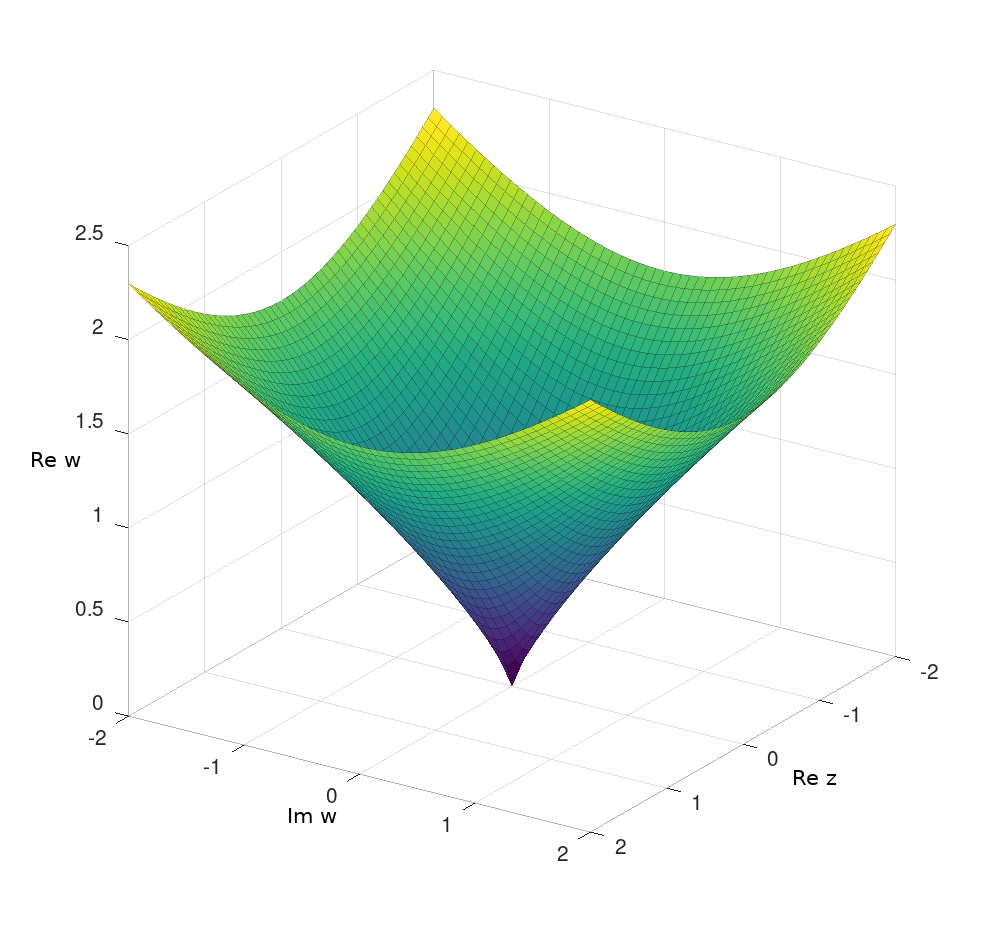
\includegraphics[width=0.7\textwidth, trim=0 4cm 0 2.5cm]{Immagini/caltrop.png} \\
        \caption{proiezione a $\mathfrak{Im}z=0$ del bordo della punta in $\mathbb{C}^2$ con coordinate $(z,w)$ corrispondente a $\psi(x)=x^{5/4}$}
    \end{center}
\end{figure}

Ci occupiamo adesso di mostrare che i domini Caltrops esistono. Vediamo l'esempio di un dominio Caltrop con una sola punta in $\mathbb{C}^2$. Siano $A,\beta>0$ e sia $\psi:[-A,\beta]\longrightarrow[0,+\infty)$ una funzione continua di classe $C^2$ su $(-A,\beta)$ tale che:
\begin{enumerate}[label={(\arabic*)}]
    \item per ogni $t\in(-A,-B)$ si ha $\psi(t)=(t+A)^p$;
    \item per ogni $t\in(0,\beta)$ si ha $\psi(t)=\sqrt{\beta^2-t^2}$,
\end{enumerate}
dove $B\in(0,A)$ e $p\in(1,3/2)$. Consideriamo il ``solido di rivoluzione'' dato da
$$\Omega:=\{(z,w)\in\mathbb{C}^2\mid |z|^2+|\mathfrak{Im}w|^2<C\psi(\mathfrak{Re}w)^2,-A<\mathfrak{Re}w<\beta\},$$
dove $C>0$ è una costante che sceglieremo più avanti.

Poniamo inoltre
$$\rho(z,w):=|z|^2+|\mathfrak{Im}w|^2-C\psi(\mathfrak{Re}w)^2,$$
considerata sull'insieme $\{(z,w)\in\mathbb{C}^2\mid -A<\mathfrak{Re}w<\beta+\epsilon\}$, dove $\epsilon>0$ è fissato e $\psi^2$ è estesa nel modo ovvio su $(\beta,\epsilon)$. Si verifica che $\rho$ è una funzione $C^2$ avente l'ipersuperficie reale $\partial\Omega\cap\{(z,w)\in\mathbb{C}^2\mid -A<\mathfrak{Re}w\}$ come luogo di zeri. Calcoliamo le seguenti derivati parziali seconde:
\begin{gather*}
    \partial^2_{z\bar{z}}\rho\equiv 1;\\
    \partial^2_{z\bar{w}}\rho=\partial^2_{\bar{z}w}\rho\equiv 0;\\
    \partial^2_{w\bar{w}}\rho(z,w)=\frac{1}{2}-\frac{C}{2}\big(\psi''(\mathfrak{Re}w)\psi(\mathfrak{Re}w)+\psi'(\mathfrak{Re}w)^2\big).
\end{gather*}

In particolare, si ha che
$$\partial^2_{w\bar{w}}\rho(z,w)-\frac{1}{2}=-\frac{Cp(2p-1)}{2}(\mathfrak{Re}w+A)^{2(p-1)}$$
per $\mathfrak{Re}w$ sufficientemente vicino a $-A$, che tende crescendo a $0$ per $\mathfrak{Re}w$ che tende descrescendo a $-A$. Allora, essendo $\psi$ di classe $C^2$ su $(-A,\beta)$, scegliendo $C$ sufficientemente piccolo possiamo imporre che $\partial^2_{w\bar{w}}\rho(z,w)\ge\dfrac{1}{4}$ per ogni $w$ tale che $-A<\mathfrak{Re}w\le 0$. Segue che $\partial\Omega\cap\{(z,w)\in\mathbb{C}^2\mid -A<\mathfrak{Re}w\le 0\}$ è un sottoinsieme di punti strettamente pseudoconvessi del bordo di $\Omega$. Per la condizione (2) su $\psi$, anche $\partial\Omega\cap\{(z,w)\in\mathbb{C}^2\mid \mathfrak{Re}w>0\}$ lo è. Le altre proprietà di dominio Caltrop seguono dalla condizione (1) su $\psi$; la punta è in $(0,-A)$.

In \cite[Section 3.2]{CMS} vengono costruiti domini Caltrops con un numero arbitrario di punte. \\

Vediamo adesso che i domini Caltrops hanno le proprietà volute. Vogliamo mostrare innanzitutto la condizione di visibilità e il fatto che non sono domini Goldilocks, per cui costituiscono una classe di esempi più ampia. Per fare ciò, vogliamo applicare il Teorema \ref{extvis} con $U=\mathbb{C}^n$, per cui $M_{\Omega,U}=M_\Omega$, e $S=\emptyset$. Per mostrare che un dominio Caltrop $\Omega$ soddisfa le ipotesi del Teorema \ref{extvis} l'idea, spiegata in \cite[Section 6]{CMS}, è la seguente: si calcola $k_D$ per un dominio planare $D$ che useremo come modello, dopodiché immergeremo copie di $D$ in $\Omega$ in maniera affine, di modo che ogni punti di $\Omega$ sufficientemente vicino al bordo sia contenuto in una di queste copie. A questo punto, useremo la Proposizione \ref{semicontr} per stimare la distanza di Kobayashi su $\Omega$. 

Per essere precisi, useremo una classe di domini con certe proprietà, che adesso andiamo a costruire. Dati $a,h>0$, poniamo
$$S_{a,h}=\{z\in\mathbb{C}\mid\mathfrak{Re}z>a\text{ e }-h<\mathfrak{Im}z<h\}.$$

Indichiamo con $T_{a,h}$ l'immagine di $S_{a,h}$ tramite la mappa $z\longmapsto 1/z$ e notiamo che
$$T_{a,h}=\left(\mathbb{C}\setminus\overline{D\left(\frac{-i}{2h},\frac{1}{2h}\right)}\right)\cap\left(\mathbb{C}\setminus\overline{D\left(\frac{i}{2h},\frac{1}{2h}\right)}\right)\cap D\left(\frac{1}{2a},\frac{1}{2a}\right).$$

Indichiamo con $\mathcal{Q}^{\alpha,a,h}$ l'immagine di $T_{a,h}$ tramite la mappa $\phi_\alpha(z)=z^{\alpha}$, dove $\alpha$ è un reale maggiore di $1$ e $a$ e $h$ sono scelti in modo che $\phi_\alpha$ sia un biolomorfismo.

Osserviamo che $T_{a,h}$ ha una cuspide quadratica in $0$. Dunque esistono due costanti $c_1,c_2>0$ tali che per ogni $z\in\partial T_{a,h}$ si ha
\begin{equation} \label{cusp_estimate}
    c_1(\mathfrak{Re}z)^2 \le |\mathfrak{Im}z| \le c_2(\mathfrak{Re}z)^2
\end{equation}
per $\mathfrak{Re}z$ sufficientemente piccola. Più precisamente, per $\delta>0$ sufficientemente piccolo l'insieme $\partial T_{a,h}\cap\{z\in\mathbb{C}\mid 0 \le \mathfrak{Re}\le\delta\}$ è dato dall'unione dei grafici di $f$ e $-f$, dove, posto $z=x+iy$, si ha $f(x)=\dfrac{1}{2h}-\sqrt{\dfrac{1}{4h^2}-x^2}$, per cui abbiamo che
\begin{equation} \label{cerchio}
    f(x)=hx^2+O(x^4)
\end{equation}
per $x\longrightarrow0^+$.

\begin{oss}
    Scrivendo l'equazione esplicita per il bordo di $\mathcal{Q}^{2,a,1}$ vicino a $0$, con $a$ sufficientemente grande, troviamo una cardioide, della quale ricordiamo la cuspide proprio in $0$. Tuttavia, sebbene semplice da calcolare, il caso $\alpha=2$ non è contemplato per via di una costrizione che imporremo più avanti.
\end{oss}

Il seguente risultato sulle proprietà dei domini $\mathcal{Q}^{\alpha,a,h}$ sarà quello usato per ottenere stime sulla distanza di Kobayashi dei domini Caltrops.

\begin{prop} \label{qaah_biolo}
    Sia $\alpha>1$ e sia $\mathcal{Q}^{\alpha,a,h}$ come sopra, con $a,h>0$ scelti opportunamente. Poniamo $p=(1+\alpha)/\alpha$; allora
    \begin{enumerate}[label={(\arabic*)}]
        \item esistono delle costanti $\epsilon,C_1,C_2>0$ tali che, per ogni $z\in\partial\mathcal{Q}^{\alpha,a,h}$ con $0\le\mathfrak{Re}z\le\epsilon$, si ha che
        $$C_1(\mathfrak{Re}z)^p \le |\mathfrak{Im}z| \le C_2(\mathfrak{Re}z)^p;$$
        \item fissata una costante $M>1$ esiste $\epsilon>0$ sufficientemente piccolo tale che la disuguaglianza al punto (1) vale con $C_2=Mh\alpha$. Inoltre, fissati $\alpha>1$ e $h>0$, tale scelta di $\epsilon$ decresce al crescere di $a$;
        \item fissiamo un punto $x_0\in\mathcal{Q}^{\alpha,a,h}\cap\mathbb{R}$. Esiste una costante $C=C(x_0)>0$ tale che per ogni $x\in(0,x_0)$ si ha che
        $$k_{\mathcal{Q}^{\alpha,a,h}}(x_0,x) \le C+\frac{\pi}{4h}x^{-1/\alpha}.$$
    \end{enumerate}
\end{prop}

\begin{proof}
    Siano $c_1$ e $c_2$ le costanti date in \eqref{cusp_estimate}, e sia $f$ la funzione di \eqref{cerchio}, cioè $f(x)=\dfrac{1}{2h}-\sqrt{\dfrac{1}{4h^2}-x^2}$. Vogliamo studiare l'immagine dei grafici di $f$ e $-f$ tramite $\phi_\alpha$. Per simmetria, ci basterò studiare l'immagine del grafico di $f$. Scriviamo $z$ nel grafico di $f$ sufficientemente vicino a $0$ come $z=x+iy$, con $x \ge 0$ e $c_1x^2\le y\le c_2x^2$. Per $x>0$ sufficientemente piccolo, svolgiamo il seguente conto:
    \begin{align*}
        \phi_\alpha(z)&=(x+iy)^{\alpha}\\
        &=x^{\alpha}\left(1+\sum_{j=1}^{+\infty}\frac{(-1)^j}{(2j)!}\prod_{\nu=0}^{2j-1}(\alpha-\nu)\frac{y^{2j}}{x^{2j}}\right)\\
        &+ix^{\alpha}\left(\sum_{j=0}^{+\infty}\frac{(-1)^j}{(2j+1)!}\prod_{\nu=0}^{2j}(\alpha-\nu)\frac{y^{2j+1}}{x^{2j+1}}\right).
    \end{align*}

    Usando il fatto che $c_1x^2\le y\le c_2x^2$, si vede facilmente che
    \begin{gather*}
        \mathfrak{Re}\big(\phi_\alpha(z)\big)=x^\alpha+O(x^{2+\alpha})\\
        \text{ e }\\
        c_1\alpha x^{1+\alpha}\big(1-O(x^2)\big) \le \mathfrak{Im}\big(\phi_\alpha(z)\big) \le c_2\alpha x^{1+\alpha}\big(1+O(x^2)\big)
    \end{gather*}
    per $z=x+iy$ nel grafico di $f$ e $x>0$ sufficientemente piccolo. Da queste disuguaglianze segue la tesi del punto (1).

    Il punto (2) segue dalle stime con le quali abbiamo dimostrato il punto (1), e da come il dominio di $f$ dipende, per costruzione, da $a$.

    Consideriamo il biolomorfismo $\Phi_{\alpha,a,h}$ da $\mathcal{Q}^{\alpha,a,h}$ in $\mathbb{D}$ dato da
    $$\Phi_{\alpha,a,h}=f_3\circ f_2\circ f_1\circ g\circ(\phi_\alpha\restrict{T_{a,h}})^{-1},$$
    dove
    \begin{align*}
        g(z)&=1/z\text{ per ogni }z\in T_{a,h},\\
        f_1(z)&=\frac{\pi i}{2h}(z-a)\text{ per ogni }z\in S_{a,h},\\
        f_2(z)&=\sin{z}\text{ per ogni }z\in \mathbb{C}\text{ con }-\pi/2<\mathfrak{Re}z<\pi/2\text{ e }\mathfrak{Im}z>0,\\
        f_3(z)&=\frac{z-i}{z+i}\text{ per ogni }z\in\mathbb{C}\text{ con }\mathfrak{Im}z>0.
    \end{align*}

    Osserviamo che $\Phi_{\alpha,a,h}$ manda l'intervallo chiuso e limitato $\overline{\mathcal{Q}^{\alpha,a,h}\cap\mathbb{R}}$ omeomorficamente in $[-1,1]$. Inoltre, manda il punto $o=\dfrac{1}{\left(\frac{2h}{\pi}\log(\sqrt{2}+1)+a\right)^\alpha}$ in $0$, e se $x\in\mathcal{Q}^{\alpha,a,h}\cap\mathbb{R}$ è minore di $o$ allora $\Phi_{\alpha,a,h}(x)\in(0,1)$. Allora per tali $x$ si ha che
    $$k_{\mathcal{Q}^{\alpha,a,h}}(o,x)=k_{\mathbb{D}}\big(0,\Phi_{\alpha,a,h}(x)\big)=\frac{1}{2}\log\left(\frac{1+\Phi_{\alpha,a,h}(x)}{1-\Phi_{\alpha,a,h}(x)}\right).$$

    Calcolando esplicitamente $\Phi_{\alpha,a,h}(x)$, troviamo che
    \begin{align*}
        \frac{1}{2}\log\left(\frac{1+\Phi_{\alpha,a,h}(x)}{1-\Phi_{\alpha,a,h}(x)}\right)&=\frac{1}{2}\log\left(e^{\frac{\pi}{2h}\left(\frac{1}{x^{1/\alpha}}-a\right)}-e^{-\frac{\pi}{2h}\left(\frac{1}{x^{1/\alpha}}-a\right)}\right)-\frac{\log{2}}{2}\\
        &\le \frac{1}{2}\log\left(e^{\frac{\pi}{2h}\left(\frac{1}{x^{1/\alpha}}-a\right)}\right) \le \frac{\pi}{4h}x^{-1/\alpha};
    \end{align*}
    usando anche la disuguaglianza triangolare, otteniamo così la tesi del punto (3).
\end{proof}

I prossimi risultati saranno quelli necessari a immergere affinamente copie di $\mathcal{Q}^{\alpha,a,h}$ in un dominio Caltrop nel modo voluto. Nel seguito, con $o$ indichiamo il punto introdotto nella dimostrazione della Proposizione \ref{qaah_biolo}, associato al dominio $\mathcal{Q}^{\alpha,a,h}$ che staremo trattando.

\begin{lm} \label{superadd}
    Siano $\epsilon>0$ e $\phi:[0,\epsilon)\longrightarrow\mathbb{R}$ una funzione continua, strettamente crescente e derivabile in $(0,\epsilon)$. Supponiamo che $\phi'$ sia strettamente crescente e che $\phi(0)=0$. Allora per ogni $(x,y)\in[0,+\infty)\times[0,+\infty)$ tale che $x+y<\epsilon$ si ha che $\phi(x+y) \ge \phi(x)+\phi(y)$.
\end{lm}

\begin{proof}
    È una banale conseguenza del teorema fondamentale del calcolo integrale.
\end{proof}

\begin{lm} \label{psierre}
    Siano $A>0$ e $\psi:[0,A]\longrightarrow[0,+\infty)$ una funzione continua che sia di classe $C^2$ su $(0,A)$, e sia $p\in(1,2)$. Supponiamo inoltre che:
    \begin{itemize}
        \item esiste una costante $C>1$ tale che $x^p/C\le\psi(x)\le Cx^p$ per ogni $x\in[0,A]$;
        \item si ha che $\psi$ è strettamente crescente;
        \item si ha che $\psi'$ è strettamente crescente su $(0,A)$.
    \end{itemize}

    Poniamo $\mathcal{R}:=\left\{z\in\mathbb{C}\mid 0<\mathfrak{Re}z<A\text{ e }|\mathfrak{Im}z|<\psi\bigl(\mathfrak{Re}z\bigr)\right\}$. Allora esistono una costante $B\in(0,A)$, un compatto $K$ che interseca $\{z\in\mathbb{C}\mid\mathfrak{Re}z=A\}$ e tale che $K\setminus\{z\in\mathbb{C}\mid\mathfrak{Re}z=A\}\subsetneq\mathcal{R}$, e due costanti $a,h>0$ tali che per ogni $x+iy\in\mathcal{R}$ con $x\le B$ si ha che:
    \begin{enumerate}[label={(\arabic*)}]
        \item vale $\bigl(\psi^{-1}(|y|)+iy\bigr)+\mathcal{Q}^{1/(p-1),a,h}\subseteq\mathcal{R}$;
        \item vale $\psi^{-1}(|y|)+o>x$;
        \item vale $\bigl(\psi^{-1}(|y|)+iy\bigr)+o\in K$;
        \item vale $\delta_{\mathcal{R}}(x+iy) \le |\psi^{-1}(|y|)-x|$.
    \end{enumerate}
\end{lm}

\begin{proof}
    Per il punto (2) della Proposizione \ref{qaah_biolo}, possiamo fissare una costante $M>1$ tale che per ogni $\alpha>1$ e ogni $a,h>0$ esiste un $\epsilon=\epsilon(\alpha,a,h)>0$ tale che
    \begin{align*}
        \mathcal{Q}^{\alpha,a,h}\cap\{\mathfrak{Re}w<\epsilon\}&\subseteq \{w\in\mathbb{C}\mid 0<\mathfrak{Re}w<\epsilon\text{ e }|\mathfrak{Im}w|<Mh\alpha(\mathfrak{Re}w)^{(1+\alpha)/\alpha}\}\\
        &=:S^{\alpha,a,h},
    \end{align*}
    e tale che, per $\alpha$ e $h$ fissati, $\epsilon\longrightarrow0$ per $a\longrightarrow+\infty$; notiamo anche che possiamo imporre $\mathcal{Q}^{\alpha,a,h}\cap\{\mathfrak{Re}w<\epsilon\}=\mathcal{Q}^{\alpha,a,h}$ per $a$ sufficientemente grande. Fissiamo adesso $\alpha=1/(p-1)$. Poiché, per costruzione di $\mathcal{Q}^{\alpha,a,h}$, a parte reale fissata di un punto del bordo la parte immaginaria decresce, la costante $\epsilon$ scelta non decresce al decrescere di $h$. Allora possiamo scegliere $a$ sufficientemente grande e $h$ sufficientemente piccolo, in modo che $\mathcal{Q}^{\alpha,a,h}\cap\{\mathfrak{Re}w<\epsilon\}=\mathcal{Q}^{\alpha,a,h}$ e $\epsilon,o<A/2$, e $Mh\alpha<1/C$.
    
    Adesso fissiamo una costante $B\in(0,A)$ tale che $B<\min\{o,\epsilon/2\}$. Sia $z=x+iy\in\mathcal{R}$ con $x\le B$. Consideriamo l'insieme $\bigl(\psi^{-1}(|y|)+iy\bigr)+\mathcal{Q}^{\alpha,a,h}$. Un elemento arbitrario di questo insieme è della forma $\bigl(\psi^{-1}(|y|)+s\bigr)+i(y+t)$, con $s+it\in\mathcal{Q}^{\alpha,a,h}$. Dato che $\mathcal{Q}^{\alpha,a,h}\subseteq S^{\alpha,a,h}$, si ha $0<s<\epsilon$ e $|t|<Mh\alpha s^p$. Il punto $\bigl(\psi^{-1}(|y|)+s\bigr)+i(y+t)$ sta in $\mathcal{R}$ se e solo \begin{gather*}
        0<\psi^{-1}(|y|)+s<A\\
        \text{e}\\
        |y+t|<\psi\big(\psi^{-1}(|y|)+s\big).
    \end{gather*}

    Poiché $x+iy\in\mathcal{R}$ e $\psi$ è strettamente crescente, si ha $0 \le \psi^{-1}(|y|)<x\le B$, per cui $0<\psi^{-1}(|y|)+s<\epsilon/2+\epsilon<A$. Dunque, per mostrare il punto (1), ci resta da dimostrare che $|y+t|<\psi\big(\psi^{-1}(|y|)+s\big)$. Notiamo che $\psi$ soddisfa le ipotesi del Lemma \ref{superadd}, da cui
    $$\psi\big(\psi^{-1}(|y|)+s\big)\ge |y|+\psi(s)\ge |y|+s^p/C,$$
    dove la prima disuguaglianza è data dal Lemma e la seconda è vera per ipotesi. Allora si ha che
    $$|y+t| \le |y|+|t|<|y|+Mh\alpha s^p<|y|+s^p/C \le \psi\big(\psi^{-1}(|y|)+s\big),$$
    come voluto.

    Per ogni $x+iy\in\mathcal{R}$ con $x\le B$ si ha $\psi^{-1}(|y|)+o>B \ge x$ per come è stato scelto $B$, e questo dimostra il punto (2).

    Definiamo $K:=\left\{z\in\mathbb{C}\mid o \le \mathfrak{Re}z\le A\text{ e }|\mathfrak{Im}z| \le \psi\big(\mathfrak{Re}(z)-o\big)\right\}$. Per ogni $x+iy\in\mathcal{R}$ con $x\le B$ si ha
    $$o \le o+\psi^{-1}(|y|) <o+x \le o+B<2o<A.$$

    Inoltre $|y|=\psi\Big(\big(\psi^{-1}(|y|)+o\big)-o\Big)$, per cui $o+\big(\psi^{-1}(|y|)+iy\big)\in K$. Per costruzione, $K$ è un compatto che soddisfa le condizioni richeste, dunque abbiamo mostrato il punto (3).

    Infine, per ogni $x+iy\in\mathcal{R}$ con $x\le B$ si ha che $\psi^{-1}(|y|)+iy\in\partial\mathcal{R}$, per cui $\delta_{\mathcal{R}}(x+iy) \le \left|\big(\psi^{-1}(|y|)+iy\big)-(x+iy)\right|=|\psi^{-1}(|y|)-x|$; questo dimostra il punto (4).
\end{proof}

Il prossimo risultato, che è sostanzialmente una versione parametrizzata del precedente, tratta dell'immersione del dominio modello $\mathcal{Q}^{\alpha,a,h}$ in un dominio Caltrop con una punta. Per brevità, scriveremo $(z_1,\dots,z_{n-1},z_n)\in\mathbb{C}^n$ come $(z',z_n)$.

\begin{lm}\label{6punto4}
    Siano $A>0$ e $\psi:[0,A]\longrightarrow[0,+\infty)$ una funzione continua che sia di classe $C^2$ su $(0,A)$, e sia $p\in(1,2)$. Supponiamo inoltre che:
    \begin{itemize}
        \item esiste una costante $C>1$ tale che $x^p/C\le\psi(x)\le Cx^p$ per ogni $x\in[0,A]$;
        \item si ha che $\psi$ è strettamente crescente;
        \item si ha che $\psi'$ è strettamente crescente su $(0,A)$.
    \end{itemize}

    Sia
    $$D:=\{z\in\mathbb{C}^n\mid 0<\mathfrak{Re}z_n<A\text{ e }(\mathfrak{Im}z_n)^2+\|z'\|^2<\big(\psi(\mathfrak{Re}z_n)\big)^2\}.$$

    Sia $w'\in\mathbb{C}^{n-1}$ e poniamo
    $$\mathcal{R}_{w'}:=\pi_n\left[\big((w',0)+\{0_{n-1}\}\times\mathbb{C}\big)\cap D\right],$$
    dove $\pi_n$ è la proiezione sull'ultima coordinata. Sia $\alpha=1/(p-1)$. Allora esistono delle costanti $a,h,B>0$ e un compatto $K\subseteq\{z\in\mathbb{C}^n\mid\mathfrak{Re}z_n\le A\}$, che interseca $\{z\in\mathbb{C}^n\mid\mathfrak{Re}z_n=A\}$ e tale che $K\setminus\{z\in\mathbb{C}^n\mid\mathfrak{Re}z_n=A\}\subsetneq D$, tali che per ogni $w'\in\mathbb{C}^{n-1}$ con $\|w'\|<\psi(B/2)$ e ogni $\zeta\in\mathcal{R}_{w'}$ con $\mathfrak{Re}\zeta\le B$ si ha che:
    \begin{enumerate}[label={(\arabic*)}]
        \item vale $\Big(\psi^{-1}\big(S(\zeta,w')\big)+i\mathfrak{Im}\zeta\Big)+\mathcal{Q}^{\alpha,a,h}\subseteq\mathcal{R}_{w'}$;
        \item vale $\psi^{-1}\big(S(\zeta,w')\big)+o>\mathfrak{Re}\zeta$;
        \item vale $\Big(\psi^{-1}\big(S(\zeta,w')\big)+i\mathfrak{Im}\zeta\Big)+o\in\pi_n\left[\big((w',0)+\{0_{n-1}\}\times\mathbb{C}\big)\cap K\right]$;
        \item vale $\delta_D\big((w',\zeta)\big) \le \left|\mathfrak{Re}\zeta-\psi^{-1}\big(S(\zeta,w')\big)\right|$,
    \end{enumerate}
    dove $S(\zeta,w')=\sqrt{(\mathfrak{Im}\zeta)^2+\|w'\|^2}$.
\end{lm}

\begin{proof}
    Notiamo che
    \begin{align*}
        \mathcal{R}_{w'}&=\{\zeta\mid (w',\zeta)\in D\}\\
        &=\{\zeta\mid0<\mathfrak{Re}\zeta<A\text{ e }(\mathfrak{Im}\zeta)^2+\|w'\|^2<\big(\psi(\mathfrak{Re}\zeta)\big)^2\}\\
        &=\{\zeta\mid \psi^{-1}(\|w'\|)<\mathfrak{Re}\zeta<A\text{ e }(\mathfrak{Im}\zeta)^2+\|w'\|^2<\big(\psi(\mathfrak{Re}\zeta)\big)^2\},
    \end{align*}
    per cui $\mathcal{R}_{w'}\not=\emptyset$ se e solo se $\|w'\|<\psi(A)$; poiché la costante $B$ sarà scelta in $(0,A)$, nel nostro caso $\mathcal{R}_{w'}$ sarà sempre non vuoto. Notiamo inoltre che l'insieme $\mathcal{R}_{0_{n-1}}$ coincide con l'insieme $\mathcal{R}$ del Lemma \ref{psierre}. Prendiamo dunque $a,h$ e $B$ date da tale Lemma. Scriviamo per semplicità $c=1/C$, e osserviamo che dalla dimostrazione del Lemma \ref{psierre} discendono le seguenti disuguaglianze:
    \begin{gather}
        B+s<3A/4<A\text{ e }|t|<cs^p\text{ per ogni }s+it\in\mathcal{Q}^{\alpha,a,h};\label{qminoredia}\\
        o>B.\label{obbi}
    \end{gather}

    Supponiamo ora che $w'\not=0_{n-1}$. Sia $\zeta\in\mathcal{R}_{w'}$ tale che $\mathfrak{Re}\zeta\le B$. Un elemento arbitrario dell'insieme $\Big(\psi^{-1}\big(S(\zeta,w')\big)+i\mathfrak{Im}\zeta\Big)+\mathcal{Q}^{\alpha,a,h}$ è della forma $\Big(\psi^{-1}\big(S(\zeta,w')\big)+s\Big)+i(\mathfrak{Im}\zeta+t)$ con $s+it\in\mathcal{Q}^{\alpha,a,h}$. Un tale punto appartiene a $\mathcal{R}_{w'}$ se e solo se:
    \begin{nlist}
        \item si ha $\psi^{-1}\big(S(\zeta,w')\big)+s<A$;
        \item si ha $\|w'\|^2+(\mathfrak{Im}w+t)^2<\bigg(\psi\Big(\psi^{-1}\big(S(\zeta,w'\big)+s)\Big)\bigg)^2$.
    \end{nlist}

    Poiché $\zeta\in\mathcal{R}_{w'}$ e $\mathfrak{Re}\zeta\le B$, abbiamo che
    $$(\mathfrak{Im}\zeta)^2+\|w'\|^2<\big(\psi(\mathfrak{Re}\zeta)\big)^2<\big(\psi(B)\big)^2;$$
    quindi $\psi^{-1}\big(S(\zeta,w')\big)+s<B+s<A$, dove l'ultima disuguaglianza è la prima in \eqref{qminoredia}. È così verificata la condizione (i). Vediamo ora la condizione (ii). Per il Lemma \ref{superadd} e per le ipotesi su $\psi$ si ha che
    $$\psi\Big(\psi^{-1}\big(S(\zeta,w'\big)+s)\Big)\ge S(\zeta,w')+\psi(s) \ge S(\zeta,w')+cs^p;$$
    dunque
    $$\bigg(\psi\Big(\psi^{-1}\big(S(\zeta,w'\big)+s)\Big)\bigg)^2-(\mathfrak{Im}\zeta)^2-\|w'\|^2\ge 2cs^pS(\zeta,w')+c^2s^{2p}.$$

    Allora la condizione (ii) segue se mostriamo che
    $$2t\mathfrak{Im}\zeta+t^2<2cs^pS(\zeta,w')+c^2s^{2p},$$
    ma quest'ultima disuguaglianza segue dalla seconda disuguaglianza in \eqref{qminoredia}. Abbiamo così dimostrato il punto (1).

    Adesso notiamo che
    $$\psi^{-1}\big(S(\zeta,w')\big)+o \ge \psi^{-1}(\mathfrak{Im}\zeta)+o>B\ge\mathfrak{Re}\zeta,$$
    dove la seconda disuguaglianza segue da \eqref{obbi}; questo dimostra il punto (2).

    Poniamo $K:=\{(w',\zeta)\in\mathbb{C}^n\mid o\le\mathfrak{Re}\zeta\le A\text{ e }S(\zeta,w')\le\psi(\mathfrak{Re}\zeta-o)\}$. Si verifica facilmente che $K$ è un compatto con le proprietà richieste. Sia $\zeta\in\mathcal{R}_{w'}$ tale che $\mathfrak{Re}\zeta\le B$ e poniamo $\eta:=\Big(\psi^{-1}\big(S(\zeta,w')\big)+i\mathfrak{Im}\zeta\Big)+o$; allora abbiamo che
    $$o\le\psi^{-1}(\|w'\|)+o\le\mathfrak{Re}\eta<\mathfrak{Re}\zeta+o\le B+o<A.$$

    Inoltre, si ha che $S(\eta,w')=S(\zeta,w')=\psi(\mathfrak{Re}\eta-o)$; quindi
    $$\eta\in\pi_n\left[\big((w',0)+\{0_{n-1}\}\times\mathbb{C}\big)\cap K\right],$$
    e questo dimostra il punto (3).

    Per il punto (4), se $(w',\zeta)$ è preso come sopra, allora
    $$\psi^{-1}\big(S(\zeta,w')\big)+i\mathfrak{Im}\zeta\in\partial\mathcal{R}_{w'};$$
    dunque
    $$\delta_D\big((w',\zeta)\big)\le \delta_{\mathcal{R}_{w'}}(\zeta)\le\left|\mathfrak{Re}\zeta-\psi^{-1}\big(S(\zeta,w')\big)\right|,$$
    come voluto.
\end{proof}

Ci serviranno anche i seguenti risultati.

\begin{lm} \label{analisibase}
    Siano $A>0$, $p>1$ e $\psi:[0,A]\longrightarrow[0,+\infty)$ una funzione tale che:
    \begin{itemize}
        \item è di classe $C^1$ su $(0,A)$;
        \item esiste $C>1$ tale che per ogni $x\in[0,A]$ si ha $\psi(x) \le Cx^{p}$;
        \item si ha che $\psi'$ è crescente su $(0,A)$.
    \end{itemize}

    Allora $\psi$ è derivabile in $0$ e $\psi'$ è continua su $[0,A)$, per cui $\displaystyle\lim_{x\longrightarrow0^+}\psi'(x)=0$.
\end{lm}

\begin{proof}
    Che $\psi'(0)$ esista e sia uguale a $0$ segue immediatamente dalla stima su $\psi(x)$. Dunque $\psi'$ si estende a una funzione su $[0,A)$. Poiché $\psi'$ è monotona crescente, esiste $\displaystyle\lim_{x\longrightarrow0^+}\psi'(x)=l<+\infty$. Segue allora da risultati elementari di analisi in una variabile che $l=0$.
\end{proof}

\begin{lm} \label{pshestimate}
    (\cite[Result 2.6]{BM})\marginpar{Sistemare con la reference originale} Siano $\Omega\subseteq\mathbb{C}^n$ un dominio e $p\in\Omega$. Supponiamo che esista una funzione $u$ plurisubarmonica, negativa, di classe $C^2$ in un intorno di $p$ e tale che esiste $c>0$ per cui si ha
    $$L_u(p;v) \ge c\|v\|^2$$
    per ogni $v\in\mathbb{C}^n$. Allora esiste una costante $\alpha>0$ tale che
    $$K_\Omega(p;v)\ge\left(\frac{c}{\alpha}\right)^{1/2}\frac{\|v\|}{|u(p)|^{1/2}}$$
    per ogni $v\in\mathbb{C}^n$.
\end{lm}

\begin{lm}\label{psdcvxcpt}
    (\cite[Result 2.4]{BM})\marginpar{Sistemare con la reference originale} Sia $\Omega\subseteq\mathbb{C}^n$ con $n\ge 2$ un dominio limitato. Sia $\mathcal{M}_0$ un insieme aperto in $\partial\Omega$ che sia anche un'ipersuperficie di classe $C^2$. Assumiamo che $\mathcal{M}_0$ ammetta una funzione di definizione $\phi$ di classe $C^2$ in un qualche aperto contenente $\mathcal{M}_0$, e tale che esista una costante $\delta>0$ per cui $L_\phi(\xi;v)\ge\sigma\|v\|^2$ per ogni $\xi\in\mathcal{M}_0$ e $v\in\mathbb{C}^n$. Sia $\mathcal{M}_1\subsetneq\mathcal{M}_0$ un sottoinsieme compatto. Allora esistono un intorno di $\mathcal{M}_1$ in $\overline{\Omega}$, sia esso $\mathcal{V}$, e due costanti $C,c>0$ tali che $K_\Omega(z;v)\ge \big(1-C\delta_\Omega(z)^{1/2}\big)\dfrac{c\|v\|}{\delta_\Omega(z)^{1/2}}$ per ogni $z\in\mathcal{V}\cap\Omega$ e $v\in\mathbb{C}^n$.
\end{lm}

Siamo ora pronti a dimostrare quello che volevamo.

\begin{thm}
    (\cite[Theorem 1.4]{BM}) Sia $\Omega$ un dominio Caltrop; allora $\Omega$ è $(\lambda,\kappa)$-visibile per ogni $\lambda \ge 1$ e $\kappa>0$, ma non è un dominio Goldilocks.
\end{thm}

\begin{proof}
    Fissiamo la seguente notazione: date due funzioni non negative $F$ e $G$ che dipendono da alcuni parametri, scriviamo $G\lesssim F$ per dire che esiste una costante $C>0$, indipendente dai parametri, tale che $G\le C\cdot F$. Scriviamo $G\approx F$ per intendere $G\lesssim F$ e $F\lesssim G$.\\

    Passo 1: una stima dal basso per $K_\Omega(w;\cdot)$ per $w$ contenuto in una punta.

    Siano $\{q_1,\dots,q_N\}\subseteq\partial\Omega$ i punti della Definizione \ref{defcaltrop}, e fissiamo $q_{j^*}$ uno di tali punti. Siano $p_{j^*}\in(1,3/2)$ l'esponente, $\mathbb{U}^{(j^*)}$ la trasformazione unitaria e $\psi_{j^*}:[0,A_{j^*}]\longrightarrow[0,+\infty)$ la funzione associati a $q_{j^*}$ nella Definizione \ref{defcaltrop}. Per la Proposizione \ref{metrdecr} abbiamo che $K_\Omega$ è invariante per biolomorfismi, e $\mathbb{U}_{j^*}$ è un biolomorfismo con differenziale $\mathbb{U}^{(j^*)}$ chee preserva la norma euclidea; allora possiamo assumere senza perdita di generalità $\mathbb{U}_{j^*}=\id$ e $q_{j^*}=0$, per cui, ponendo $A=A_{j^*}$ e $\psi=\psi_{j^*}$, si ha che
    $$\Omega\cap V_{j^*}=\left\{z\in\mathbb{C}^n\mid 0<\mathfrak{Re}z_n<A\text{ e }(\mathfrak{Im}z_n)^2+\|z'\|^2<\big(\psi(\mathfrak{Re}z_n)\big)^2\right\}.$$

    Poniamo $\rho(z):=(\mathfrak{Im}z_n)^2+\|z'\|^2-\big(\psi(\mathfrak{Re}z_n)\big)^2$ per $z\in\Omega\cap V_{j^*}$. Calcolando le derivate parziali seconde in modo analogo a come fatto nella costruzione dell'esempio a una punta, ricordando le proprietà di $\psi$ e applicando il Lemma \ref{analisibase}, troviamo che esiste una costante $A'\in(0,A]$ tale che
    $$L_\rho(z;v) \ge \|v'\|^2+|v_n|^2/4$$
    per ogni $z\in\Omega\cap V_{j^*}$ con $0<\mathfrak{Re}z_n<A'$ e $v\in\mathbb{C}^n$.

    Siano $U^{(\nu)}$, per $\nu=1,2,3,4$, degli intorni aperti e connessi di $0$ tali che:
    \begin{itemize}
        \item si ha $U^{(1)}\subset\subset U^{(2)}\subset\subset U^{(3)}\subset\subset U^{(4)}$;
        \item si ha $U^{(\nu)}\cap\Omega=\{z\in\Omega\cap V_{j^*}\mid0<\|z\|<\nu A'/4\}$ per $\nu=1,2,3,4$.
    \end{itemize}

    Sia $\chi_1:\mathbb{C}^n\longrightarrow[0,1]$ una funzione liscia con $\chi_1\restrict{U^{(1)}}\equiv 0$ e $\chi_1\restrict{\mathbb{C}^n\setminus U^{(2)}}\equiv 1$, e sia $\phi:[0,+\infty)\longrightarrow[0,+\infty)$ una funzione liscia con le seguenti proprietà:
    \begin{itemize}
        \item è convessa e non decrescente;
        \item è nulla in $[0,(A')^2/16]$;
        \item crece lentamente nell'intervallo $((A')^2/16,(A')^2/4]$;
        \item cresce rapidamente nell'intervallo $[9(A')^2/16,+\infty)$.
    \end{itemize}

    A breve specificheremo cosa intendiamo di preciso con le ultime due condizioni, ma per farlo ci serviranno altre funzioni che adesso definiamo. Poniamo $M_\phi:=\displaystyle\sup_{z\in\Omega}\phi(\|z\|^2)$ e $\Phi(z):=\phi(\|z\|^2)-M_\phi$ per ogni $z\in\Omega$. Abbiamo che $\Phi$ è plurisubarmonica per \cite[Proposition 2.2.6]{Kr}.\marginpar{È lecito citarlo, anche se le dimostrazioni rilevanti sono lasciate per esercizio?} Si ha allora che
    \begin{align*}
        L_{\rho+\chi_1\Phi}(z;v)&=L_\rho(z;v)+\chi_1(z)L_\Phi(z;v)\\
        &+2\mathfrak{Re}\left(\sum_{j,k=1}^n\partial_{z_j}\chi_1(z)\partial_{\bar{z}_k}\Phi(z)v_j\bar{v}_k\right)+\Phi(z)L_{\chi_1}(z;v)\\
        &\ge \|v'\|^2+|v_n|^2/4-2\sum_{j,k=1}^n|\partial_{z_j}\chi_1(z)\partial_{\bar{z}_k}\Phi(z)||v_j||\bar{v}_k|\\
        &-|\Phi(z)||L_{\chi_1}(z;v)|
    \end{align*}
    per ogni $z\in(U^{(2)}\setminus U^{(1)})\cap\Omega$ e $v\in\mathbb{C}^n$. Specifichiamo adesso la prima condizione di crescita di $\phi$. Sull'intervallo $((A')^2/16,(A')^2/4]$ deve crescere così lentamente che
    $$L_{\rho+\chi_1\Phi}(z;v)\ge 2\|v'\|^2+|v_n|^2/8$$
    per ogni $z\in(U^{(2)}\setminus U^{(1)})\cap\Omega$ e $v\in\mathbb{C}^n$.

    Sia adesso $\chi_2:\mathbb{C}^n\longrightarrow[0,1]$ una funzione liscia e a supporto compatto tale che $\chi_2\restrict{U^{(3)}}\equiv1$ e $\chi_2\restrict{\mathbb{C}^n\setminus{U^{(4)}}}\equiv 0$, e chiediamo che il supporto di $\chi_2$ intersecato con $\Omega$ sia contenuto in $\{z\in\Omega\mid \|z\|<7A'/8\}$. Abbiamo allora che
    \begin{align*}
        L_{\chi_2\rho+\Phi}(z;v)&\ge \phi'(\|z\|^2)\|v\|^2+\phi''(\|z\|^2)|\langle z,v\rangle|^2\\
        &-2\sum_{j,k=1}^n|\partial_{z_j}\chi_2(z)\partial_{\bar{z}_k}\rho(z)||v_j||\bar{v}_k|-|\rho(z)||L_{\chi_2}(z;v)|
    \end{align*}
    per ogni $z\in(U^{(4)}\setminus U^{(3)})\cap\Omega$ e $v\in\mathbb{C}^n$. Specifichiamo adesso la seconda condizione di crescita di $\phi$. Sull'intervallo $[9(A')^2/16,+\infty)$ deve crescere così lentamente che esiste una costante $c>0$ tale che
    $$L_{\chi_2\rho+\Phi}(z;v)\ge c\|v\|^2$$
    per ogni $z\in(U^{(4)}\setminus U^{(3)})\cap\Omega$ e $v\in\mathbb{C}^n$.

    Poniamo ora $u(z):=\chi_1(z)\Phi(z)+\chi_2(z)\rho(z)$. Ricordiamo che $\Phi$ è plurisubarmonica; allora:
    \begin{itemize}
        \item per il principio del massimo (\cite[Corollary 2.1.5]{Kr}, segue facilmente dalla Definizione \ref{psh} che vale anche per funzioni plurisubarmoniche) applicato a $\Phi$, e per le definizioni di $\chi_1$,$\chi_2$ e $\rho$, abbiamo che $u<0$ su $\Omega$;
        \item dalle disuguaglianze sulla forma di Levi che seguono dalle condizioni imposte su $\phi$, e dalle definizioni di $\chi_1$ e $\chi_2$, segue per\marginpar{Qua la citazione mi piace ancora meno} \cite[Excercise prior to Proposition 2.2.6]{Kr} che $u$ è plurisubarmonica su $\Omega$.
    \end{itemize}

    Per la simmetria di rotazione della punta $\Omega\cap V_{j^*}$, per ogni $w\in\Omega\cap V_{j^*}$ con $\mathfrak{Re}w_n$ sufficientemente piccolo si ha che $\delta_\Omega(w)=\text{dist}\big(\mathfrak{Re}w_n+iS(w),\text{graph}(\psi)\big)$, dove con $\text{graph}(\psi)$ s'intende il grafico di $\psi$ e $S(w)=\sqrt{(\mathfrak{Im}w_n)^2+\|w'\|^2}$. Segue dunque, da semplici stime geometriche e dal Lemma \ref{analisibase}, ponendo $\xi^w_n=\pi_n(\xi^w)$, che
    \begin{equation}\label{limite_brutto}
        \frac{\delta_\Omega(w)}{\psi(\mathfrak{Re}w_n)-S(w)}=\frac{\left|(\mathfrak{Re}\xi^w_n-\mathfrak{Re}w_n)+i\big(\psi(\mathfrak{Re}\xi^w_n)-S(w)\big)\right|}{\psi(\mathfrak{Re}w_n)-S(w)}\longrightarrow 1
    \end{equation}
    per $\mathfrak{Re}w_n\longrightarrow 0$. Allora esiste una costante $A''>0$ tale che:
    \begin{gather}
        \{z\in\Omega\cap V_{j^*}\mid0<\mathfrak{Re}z_n<A''\}\subseteq\Omega\cap U^{(1)};\label{7punto4}\\
        \psi(x)\in(0,1)\text{ per ogni }x\in(0,A'');\label{7punto4due}\\
        \frac{\delta_\Omega(w)}{\psi(\mathfrak{Re}w_n)-S(w)}>1/2\label{7punto5}
    \end{gather}
    per ogni $w\in\Omega\cap V_{j^*}$ tale che $\mathfrak{Re}w_n\in(0,A'')$.

    Fissiamo ora un punto $w\in\Omega\cap V_{j^*}$ tale che $0<\mathfrak{Re}w_n<A''$; allora esiste una costante $b>0$ tale che
    \begin{equation}\label{7punto6}
        \begin{aligned}
            K_\Omega(w;v)&\ge b\frac{\|v\|}{|u(w)|^{1/2}}\\
            &=b\frac{\|v\|}{\big(\psi(\mathfrak{Re}w_n)-S(w)\big)^{1/2}\big(\psi(\mathfrak{Re}w_n)+S(w)\big)^{1/2}}\\
            &\ge\frac{b}{\sqrt{2}}\cdot\frac{\|v\|}{\big(\psi(\mathfrak{Re}w_n)-S(w)\big)^{1/2}} \ge \frac{b}{2}\cdot\frac{\|v\|}{\delta_\Omega(w)^{1/2}},
        \end{aligned}
    \end{equation}
    dove la prima disuguaglianza segue dal Lemma \ref{pshestimate}, l'uguaglianza segue da \eqref{7punto4} e dalle definizioni di $\chi_1$ e $\chi_2$, e la penultima e ultima disuguaglianza seguono, rispettivamente, da \eqref{7punto4due} e da \eqref{7punto5}.\\

    Passo 2: una stima dall'alto per $M_\Omega$.

    Dato che le stime fatte al passo 1 valgono per un qualsiasi $q_{j^*}$, che sono in numero finito, ne deduciamo che esistono delle costanti $\beta,A_1'',\dots,A_N''>0$ tali che
    \begin{equation}\label{7punto7}
        K_\Omega(w;v)\ge\beta\frac{\|v\|}{\delta_\Omega(w)^{1/2}}
    \end{equation}
    per ogni $w\in\Omega\cap\mathbb{U}_j^{-1}(\{z\mid\in\mathbb{C}^n\mid \mathfrak{Re}z_n<A_j''\})$, per ogni $v\in\mathbb{C}^n$ e per $j=1,\dots,N$. Adesso poniamo
    \begin{gather*}
        \mathcal{M}_0:=\partial\Omega\cap\bigcap_{j=1}^N \mathbb{U}_j^{-1}(\{z\in\mathbb{C}^n\mid \mathfrak{Re}z_n>A_j''/2\}),\\
        \mathcal{M}_1:=\partial\Omega\setminus\bigcup_{j=1}^N \mathbb{U}_j^{-1}(\{z\in\mathbb{C}^n\mid \mathfrak{Re}z_n<A_j''\}).
    \end{gather*}
    
    Dalla Definizione \ref{defcaltrop}, in ogni punto di $\partial\Omega\setminus\{q_1,\dots,q_N\}$ esiste una funzione di definizione locale. Poiché $\mathcal{M}_0$ è relativamente compatto in $\partial\Omega$, usando delle partizioni dell'unità possiamo incollare tra loro un numero finito di tali funzioni per ottenere una funzione di definzione per $\mathcal{M}_0$; siccome possiamo sempre farlo in modo che vicino a un punto specifico sia uguale alla funzione di definizione locale per $\partial\Omega\setminus\{q_1,\dots,q_N\}$, e dato che la stretta pseudoconvessità in un punto è indipendente dalla funzione di definizione scelta (\cite[Section 3.2]{Kr}), usando anche \cite[Proposition 3.2.1]{Kr} si trova che $\mathcal{M}_0$ soddisfa le ipotesi del Lemma \ref{psdcvxcpt}.

    Dunque esistono un intorno $\mathcal{V}$ di $\mathcal{M}_1$ in $\overline{\Omega}$ e una costante $\beta'>0$ tali che
    \begin{equation}\label{7punto8}
        K_\Omega(w;v)\ge \beta'\frac{\|v\|}{\delta_\Omega(w)^{1/2}}
    \end{equation}
    per ogni $w\in\mathcal{V}\cap\Omega$ e $v\in\mathbb{C}^n$. Consideriamo adesso l'insieme
    $$\Omega\setminus\left(\mathcal{V}\cup\bigcup_{j=1}^N \mathbb{U}_j^{-1}(\{z\in\mathbb{C}^n\mid\mathfrak{Re}z_n<A_j''\})\right),$$
    che è compatto per definizione; allora la pseudometrica di Kobayashi ha un minimo positivo su tale insieme. Per la \eqref{7punto7} e la \eqref{7punto8}, segue che
    $$\frac{1}{K_\Omega(w;v)}\lesssim\delta_\Omega(w)^{1/2}$$
    per ogni $w\in\Omega$ e per ogni $v\in\mathbb{C}^n$ con $\|v\|=1$. In particolare, $M_\Omega(r)\lesssim r^{1/2}$.\\

    Passo 3: il comportamento di $k_\Omega$.

    Fissiamo inizialmente un punto $q_j$, e siano $a_j$, $h_j$ e $B_j$ le costanti date dal Lemma \ref{6punto4} con $\psi=\psi_j$. Per semplicità di notazione poniamo $a=a_j$ e $h=h_j$. Consideriamo un punto $w\in\Omega\cap\mathbb{U}_j^{-1}(\{z\in\mathbb{C}^n\mid\mathfrak{Re}z_n<B_j/2\})$ e scriviamo $\mathbb{U}_j(w)=(\omega',\omega_n)$. Sia $\Psi_{j,w}:\mathcal{Q}^{\alpha,a,h}\longrightarrow\mathbb{C}^n$ la funzione olomorfa data da
    $$\psi_{j,w}(\zeta):=\mathbb{U}_j^{-1}\Big(\omega',\psi_j^{-1}\big(S(\omega)\big)+i\mathfrak{Im}\omega_n+\zeta\Big),$$
    con $\alpha=1/(p_j-1)$ e $S(\omega)=\sqrt{(\mathfrak{Im}\omega_n)^2+\|\omega'\|^2}$. Notiamo che questa mappa è un'immersione affine di $\mathcal{Q}^{\alpha,a,h}$ in $\mathbb{C}^n$. Vogliamo vedere che è un'immersione a valori in $\Omega$, per potervi ottenere la stime per $k_\Omega$.

    Notiamo che $\mathfrak{Re}\omega_n<B_j/2$; allora, per come è stato preso $w$ e per la Definizione \ref{defcaltrop}, si ha $\|\omega'\|<\psi_j(B_j/2)$. Segue quindi dai punti (1) e (2) del Lemma \ref{6punto4} che:
    \begin{nlist}
        \item si ha
        \begin{align*}
            \{\omega'\}&\times\Big(\psi_j^{-1}\big(S(\omega)\big)+i\mathfrak{Im}\omega_n+\mathcal{Q}^{\alpha,a,h}\Big)\\
            &\subseteq \{(z',z_n)\in\mathbb{C}^n\mid\mathfrak{Re}z_n\in(0,A_j)\text{ e }(\mathfrak{Im}z_n)^2+\|z'\|^2<\psi_j(\mathfrak{Re}z_n)^2\};
        \end{align*}
        \item si ha $\mathfrak{Re}\omega_n\in\Big(\psi_j^{-1}\big(S(\omega)\big),\psi_j^{-1}\big(S(\omega)\big)+o\Big)$.
    \end{nlist}

    Adesso poniamo $K_j:=\mathbb{U}_j^{-1}(K)$ e $z_w:=\Psi_{j,w}(o)$, dove $K$ è il compatto dato dal Lemma \ref{6punto4}. Allora segue, dalla parte (3) del Lemma, che
    \begin{equation}\label{7punto9}
        z_w\in K_j
    \end{equation}
    per ogni $w\in\Omega\cap V_j$ tale che $0<\mathfrak{Re}\omega_n<B_j/2$.

    Dal punto (i) sopra segue che $\Psi_{j,w}(\mathcal{Q}^{\alpha,a,h})\subseteq\Omega$. Per definizione abbiamo che $\Psi_{j,w}\Big(-\psi_j^{-1}\big(S(\omega)\big)+\mathfrak{Re}\omega_n\Big)=w$. Allora, per la Proposizione \ref{semicontr}, si ha $k_\Omega(z_w,w)\le k_{\mathcal{Q}^{\alpha,a,h}}\Big(o,-\psi_j^{-1}\big(S(\omega)\big)+\mathfrak{Re}\omega_n\Big)$. Dal punto (ii) e dalla Proposizione \ref{qaah_biolo} con $x_0=o$ troviamo che esiste una costante $C^{(j)}>0$ tale che $k_\Omega(z_w,w)\le C^{(j)}+\dfrac{\pi}{4h}\left|\mathfrak{Re}\omega_n-\psi_j^{-1}\big(S(\omega)\big)\right|^{-(p_j-1)}$. Dato che $\mathbb{U}_j$ preserva le distanze euclidee, quest'ultima disuguaglianza insieme al punto (4) del Lemma \ref{6punto4} ci dicono che
    \begin{equation}\label{7punto10}
        k_\Omega(z_w,w) \le C^{(j)}+\frac{\pi}{4h}\delta_\Omega(w)^{-(p_j-1)}
    \end{equation}
    per ogni $w\in\Omega\cap V_j$ tale che $0<\mathfrak{Re}\omega_n<B_j/2$. Siccome il punto $q_j$ è stato scelto arbitrariamente, la \eqref{7punto9} e la \eqref{7punto10} valgono per ogni $j=1,\dots,N$.

    Dato che $\partial\Omega$ è di classe $C^2$ all'infuori dei punti $q_1,\dots,q_N$ e $\Omega$ è limitato, esistono un compatto $K_0\subseteq\Omega$ e una costante $R>0$ tali che per ogni punto
    \begin{equation}\label{7punto11}
        w\in\Omega\setminus\left(K_0\cup\bigcup_{j=1}^N\mathbb{U}_j^{-1}(\{z\in\mathbb{C}^n\mid\mathfrak{Re}z_n<B_j/2\})\right)
    \end{equation}
    esiste un punto
    $$\xi^w\in\partial\Omega\setminus\bigcup_{j=1}^N\mathbb{U}_j^{-1}(\{z\in\mathbb{C}^n\mid\mathfrak{Re}z_n<B_j/4\})$$
    tale che, detto $\eta^w$ il vettore unitaro normale a $\partial\Omega$ entrante in $\xi^w$, allora:
    \begin{itemize}
        \item si ha $\xi^w+D(R;R)\eta^w\subseteq \Omega$;
        \item si ha che $w$ appartiene al segmento congiungente $\xi^w$ a $\xi^w+R\eta^w=:z^w$;
        \item si ha $z^w\in K_0$.
    \end{itemize}
    Per trovare $K_0$ e $R$, basta considerare un intorno tubolare dato \cite[Chapter 9, Theorem 20]{S}. Chiediamo anche che $\delta_\Omega(w)<1$ per ogni $w\not\in K_0$. Per ogni tale $w$ esiste un unico numero $t(w)\in(0,R)$ tale che $\xi^w+t(w)\eta^w=w$. Da ciò, e dalla Proposizione \ref{semicontr}, segue che
    \begin{equation}\label{7punto12}
        \begin{aligned}
            k_\Omega(z^w,w)&\le k_{D(R;R)}\big(0,1-t(w)\big)=\frac{1}{2}\log\left(\frac{2-t(w)/R}{t(w)/R}\right)\\
            &\le\log{\sqrt{2R}}+\frac{1}{2}\log\left(\frac{1}{\|\xi^w-w\|}\right)\le\log{\sqrt{2R}}+\frac{1}{2}\log\left(\frac{1}{\delta_\Omega(w)}\right)
        \end{aligned}
    \end{equation}
    per ogni $w$ che soddisfa la \eqref{7punto11}. Fissiamo ora un punto $z_0\in\Omega$e  poniamo
    \begin{gather*}
        K^*:=K_0\cup K_1\cup\dots\cup K_N\\
        \text{e}\\
        C_0:=\displaystyle\sup_{x\in K^*}k_\Omega(z_0,x)+\max\{\log{\sqrt{2R}},C^{(1)},\dots,C^{(N)}\};
    \end{gather*}
    allora, dalla disuguaglianza triangolare per $k_\Omega$, dalla \eqref{7punto9} e dalle disuguaglianze \eqref{7punto10} e \eqref{7punto12}, troviamo che esiste una costante $C_1>0$ tale che
    $$k_\Omega(z_0,z)\le C_0+C_1\delta_\Omega(z)^{-\max_{j=1,\dots,N}p_j+1}$$
    per ogni $z\in\Omega$.\\

    Passo 4: $\Omega$ è $(\lambda,\kappa)$-visibile per ogni $\lambda\ge 1$ e $\kappa>0$.

    Poniamo $p_0:=\displaystyle\max_{j=1,\dots,N} p_j$; abbiamo $p_0\in(1,3/2)$ per ipotesi. Per mostrare la tesi di questo passaggio, ci basterà verificare le ipotesi del Teorema \ref{extvis}. Prendendo $S=\emptyset$ e $f(r)=C_0+C_1r^{p_0-1}$, e usando i passaggi 2 e 3 dimostrati sopra, la verifica è immediata.\\

    Passo 5: $\Omega$ non è un dominio Goldilocks.

    Vogliamo mostrare che la condizione (2) nella Definizione \ref{gold} non è soddisfatta da $\Omega$. Per farlo, fissiamo un punto $q_{j^*}$; come fatto al passo 1, ci restringiamo a $\Omega\cap V_{j^*}$. Riprendendo la notazione di quel passaggio, prendiamo $A=A_{j^*}$, $A''=A_{j^*}''$, $\psi=\psi_{j^*}$, $q_{j^*}=0$ e $p=p_{j^*}$. Sia $z_0=(0,\dots,0,A''/2)$; mostriamo che per ogni $z\in\Omega\cap V_{j^*}$ tale che $0<\mathfrak{Re}z_n<A''/2$ si ha
    \begin{equation}\label{7punto14}
        k_\Omega(z_0,z)\gtrsim(\mathfrak{Re}z_n)^{-(p-1)}-(A''/2)^{-(p-1)}.
    \end{equation}

    Fissiamo uno $z$ che soddisfa le suddette condizioni. Sia $\gamma:[0,1]\longrightarrow\Omega$ una curva $C^1$ a tratti tale che $\gamma(0)=z_0$, $\gamma(1)=z$ e $\gamma([0,1))\subseteq\Omega\cap V_{j^*}$. Detta $\gamma_n$ l'ultima coordinata di $\gamma$, per continuità di $\mathfrak{Re}\gamma_n$, e con considerazioni elementari, troviamo che esistono $\alpha,\beta\in[0,1]$ tali che $(\mathfrak{Re}\gamma_n)([\alpha,\beta])=[\mathfrak{Re}z_n,A''/2]$. Quindi
    $$\int_0^1 K_\Omega\big(\gamma(t);\gamma'(t)\big)\diff t\ge\int_\alpha^\beta K_\Omega\big(\gamma(t);\gamma'(t)\big)\diff t\ge \int_\alpha^\beta \frac{b\|\gamma'(t)\|}{\left|u\big(\gamma(t)\big)\right|^{1/2}}\diff t,$$
    dove la seconda disuguaglianza segue dalla \eqref{7punto6}. Per ogni $w\in\Omega\cap V_{j^*}$ con $0<\mathfrak{Re}w_n<A''$ si ha
    $$|u(w)|=\big(\psi(\mathfrak{Re}w_n)\big)^2-\|w'\|^2-(\mathfrak{Im}w_n)^2 \le \big(\psi(\mathfrak{Re}w_n)\big)^2 \le C^2(\mathfrak{Re}w_n)^{2p},$$
    dove abbiamo preso $C=C_{j^*}$. Combinando con la disuguaglianza precedente, troviamo
    \begin{align*}
        \int_0^1 K_\Omega\big(\gamma(t);\gamma'(t)\big)\diff t&\ge \frac{b}{C}\int_\alpha^\beta \frac{|(\mathfrak{Re}\gamma_n)'(t)|}{\big((\mathfrak{Re}\gamma_n)(t)\big)^p}\diff t\\
        &\ge \left|\frac{b}{C}\int_\alpha^\beta \frac{(\mathfrak{Re}\gamma_n)'(t)}{\big((\mathfrak{Re}\gamma_n)(t)\big)^p}\diff t\right|=\frac{b}{C}\int_{\mathfrak{Re}z_n}^{A''/2}\frac{1}{t^p}\diff t,
    \end{align*}
    dove il cambio di variabile nell'ultimo passaggio non è propriamente consentito ($\mathfrak{Re}\gamma_n$ potrebbe non essere monotona su $[\alpha,\beta]$), ma possiamo farlo su un numero finito di intervalli dove è monotona e la cui immagine partiziona $[\mathfrak{Re}z_n,A''/2]$, mentre i pezzi rimanenti possiamo assorbirli nella precedente disuguaglianza. La disuguaglianza \eqref{7punto14} segue applicando il Teorema \ref{lung_int}.

    Poniamo adesso $\mu^x:=(0,\dots,0,x)$ per $0<x<A''/2$. Per la \eqref{7punto14} si ha che
    $$k_\Omega(z_0,\mu^x) \gtrsim x^{-(p-1)}-(A''/2)^{-(p-1)}.$$
    
    Dalla \eqref{limite_brutto} segue che $\delta_\Omega(\mu^x) \approx x^p$ per $x\in(0,A''/2)$. Dunque, combinando con la disuguaglianza precedente, abbiamo
    $$k_\Omega(z_0,\mu^x) \gtrsim \delta_\Omega(\mu^x)^{-1+1/p}-(A''/2)^{-(p-1)}.$$

    Dato che $p=p_{j^*}>1$, si ha $\dfrac{\delta_\Omega(\mu^x)^{-1+1/p}}{\log\left(\frac{1}{\delta_\Omega(\mu^x)}\right)}\longrightarrow +\infty$ per $\mu^x\longrightarrow 0=q_{j^*}$. Quindi $k_\Omega(z_0,\mu^x)$ non può soddisfare la condizione (2) nella Definizione \ref{gold}, come voluto. Questo conclude la dimostrazione.
\end{proof}
\subsection{Un altro esempio}
L'ultimo esempio è quello mostrato in \cite[Section 5.2]{CMS}; si tratta di un altro esempio di dominio non di tipo Goldilocks che soddisfa la condizione di visibilità.

Iniziamo considerando la funzione $\Phi_0:\mathbb{C}^2\longrightarrow\mathbb{R}$ definita da
$$\Phi_0(z):=\begin{cases}
    \exp(-1/\|z\|^2)-\mathfrak{Im}(z_2) &\mbox{se }z=(z_1,z_2)\not=(0,0)\\
    0 &\mbox{se }z=0.
\end{cases}$$

Poiché la matrice hessiana di $\Phi_0$ (vista come funzione da $\mathbb{R}^4$ in $\mathbb{R}$) è la stessa della funzione $\exp(-1/\|z\|^2)$ estesa a $0$ nell'origine, che è convessa vicino all'origine, esiste $0<\epsilon<1$ tale che $\Phi_0$ è convessa in $\mathbb{B}^2_{2\epsilon}$. Scegliamo inoltre una funzione liscia $\psi:\mathbb{C}^2\longrightarrow[0,1]$ tale che $\psi\equiv 1$ in $\mathbb{B}^2_{2\epsilon}$ e $\text{supp}\,{\psi}\subseteq \mathbb{B}^2_{3\epsilon}$. Poniamo $\Phi:=\Phi_0\cdot\psi$ e $c_0:=\displaystyle\sup_{z\in\mathbb{C}^2}\big(-\Phi(z)\big)>0$.

Scegliamo adesso una funzione liscia $\chi:[0,+\infty)\longrightarrow[0,+\infty)$ che sia identicamente nulla in $[0,\epsilon^2]$, strettamente crescente in $[\epsilon^2,+\infty)$ e strettamente convessa in $\big(\epsilon^2,(\epsilon+\delta)^2\big)$ per $0<\delta<\epsilon$; per esempio, possiamo prendere $\chi(t)=\exp\big(-1/(t-\epsilon^2)\big)$ per $t>\epsilon^2$ e $0$ altrove. Poniamo $c_1:=\chi\big((\epsilon+\delta/2)^2\big)$ e $C:=c_0/c_1$. Definiamo
$$\Psi(z):=C\chi(\|z\|^2)$$
per ogni $z\in\mathbb{C}^2$.

Osserviamo che:
\begin{itemize}
    \item la funzione $\Psi$ è liscia e non negativa su tutto $\mathbb{C}^2$, nulla in $\overline{\mathbb{B}^2_\epsilon}$, e strettamente convessa e strettamente positiva in $\mathbb{B}^2_{\epsilon+\delta}\setminus\overline{\mathbb{B}^2_\epsilon}$;
    \item si ha $\Psi(z)\ge c_0$ per ogni $z\in\mathbb{C}^2\setminus\mathbb{B}^2_{\epsilon+\delta/2}$, da cui $\Psi(z)+\Phi(z)\ge 0$ per ogni $z\in\mathbb{C}^2\setminus\mathbb{B}^2_{\epsilon+\delta/2}$;
    \item si ha $\Psi(z)+\Phi(z)=\Phi(z)=\Phi_0(z)$ per ogni $z\in\mathbb{B}^2_\epsilon$.
\end{itemize}

Consideriamo il dominio
$$\Omega:=\{z=(z_1,z_2)\in\mathbb{C}^2\mid \rho(z):=\Psi(z)+\Phi(z)<0\}.$$

Notiamo che $\Omega\subseteq\mathbb{B}^2_{\epsilon+\delta/2}$, dove $\rho=\Psi+\Phi_0$, che è una funzione convessa; per cui $\Omega$ è un dominio convesso limitato. Calcolando il gradiente di $\rho$, vediamo che esiste al più un punto $p_0\in\partial\Omega$ dove il gradiente si annulla, che è della forma $p_0=(0,ic)$; inoltre, $p_0\in\overline{\mathbb{B}^2_{\epsilon+\delta/2}}\setminus\overline{\mathbb{B}^2_\epsilon}$. Dunque $\Omega$ è un dominio limitato e convesso tale che $\partial\Omega\setminus\{p_0\}$ è liscio. Si ha anche che ogni punto di $(\partial\Omega\setminus\{p_0\})\cap(\mathbb{B}^2_{\epsilon+\delta}\setminus\overline{\mathbb{B}^2_\epsilon})$ è un punto del bordo di $\Omega$ strettamente convesso (perché in $\mathbb{B}^2_{\epsilon+\delta}\setminus\overline{\mathbb{B}^2_\epsilon}$ la funzione $\Psi$ è strettamente convessa e la funzione $\Phi_0$ è convessa); dunque è pseudoconvesso (segue dalla dimostrazione di \cite[Proposition 2.1.13]{A1}) e, per \cite[Corollary 5.6]{D'A}, è un punto di tipo finito. Poniamo $A:=\partial\Omega\cap\overline{\mathbb{B}^2_\epsilon}$ e osserviamo che
$$A=\overline{\mathbb{B}^2_\epsilon}\cap\{z\in\mathbb{C}^2\mid \Phi_0(z)=0\};$$
si ha anche che ogni punto di $A$ diverso da $(0,0)$ è un punto del bordo di $\Omega$ di tipo finito (perché $\Phi_0$ è strettamente convessa in $\overline{\mathbb{B}^2_\epsilon}\setminus\{(0,0)\}$, per cui ogni punto di $A$ è strettamente convesso). \\

Possiamo ora procedere a dimostrare che $\Omega$ è $(\lambda,\kappa)$-visibile per ogni $\lambda \ge 1$ e $\kappa>0$.

\begin{prop} \label{safinisvis}
    (\cite[Corollary 1.10]{CMS}) Sia $\Omega$ un dominio limitato di $\mathbb{C}^d$. Supponiamo che esista un compatto $S\subseteq\partial\Omega$ tale che $S_a$, l'insieme dei punti di accumulazione di $S$, sia finito, e inoltre che ogni punto $p\in\partial\Omega\setminus S$ sia un punto liscio di bordo pseudoconvesso e di tipo finito. Allora $\Omega$ è $(\lambda,\kappa)$-visibile per ogni $\lambda \ge 1$ e $\kappa>0$.
\end{prop}

\begin{proof}
    Mostriamo che, dati $p,q\in\partial\Omega$ con $p\not=q$, sono soddisfatte le ipotesi (i) e (ii) del Teorema \ref{extvis}. Per farlo, consideriamo $S_0:=S_a\cup\{p,q\}$. Allora, per finitezza di $S_0$, esiste $\epsilon_0>0$ tale che $\overline{B(x,\epsilon_0)}\cap\overline{B(x',\epsilon_0)}=\emptyset$ per ogni $x,x'\in S_0$. Adesso poniamo
    $$S_1:=(S\cup\{p,q\})\setminus\left(\bigcup_{x\in S_a}\overline{B(x,\epsilon_0)}\right);$$
    notiamo che $S_1$ è un insieme finito disgiunto dal compatto $K:=\displaystyle\bigcup_{x\in S_a}\overline{B(x,\epsilon_0)}$. Dunque esiste $\epsilon_1>0$ tale che:
    \begin{itemize}
        \item si ha $\overline{B(y,\epsilon_1)}\cap K=\emptyset$ per ogni $y\in S_1$;
        \item $\overline{B(y,\epsilon_1)}\cap\overline{B(y',\epsilon_1)}=\emptyset$ per ogni $y,y'\in S_1$ con $y\not=y'$.
    \end{itemize}
    
    Distinguiamo ora due casi. \\

    Caso 1: $p\not\in K$.

    Basta prendere $p'=p$ e $r=\epsilon_1$. \\

    Caso 2: $p\in K$.

    In questo caso esiste un $x_0\in S_a$ tale che $p\in\overline{B(x_0,\epsilon_0)}$. Consideriamo la seguente famiglia di insiemi con chiusure mutualmente disgiunte:
    $$\mathcal{B}:=\{B(x,\epsilon_0)\mid x\in S_a\}\cup\{B(y,\epsilon_1)\mid y\in S_1\};$$
    allora esiste $\epsilon_2>0$ tale che $\epsilon_2<\text{dist}(B_1,B_2)/4$ per ogni $B_1,B_2\in\mathcal{B}$. Segue che $\mathcal{C}:=\{B(x,\epsilon_0+\epsilon_2)\mid x\in S_a\}\cup\{B(y,\epsilon_1+\epsilon_2)\mid y\in S_1\}$ è una famiglia di insiemi con chiusure mutualmente disgiunte. Allora basta prendere $p'=x_0$ e $r=\epsilon_1+\epsilon_2$. \\

    Per concludere mostriamo adesso che, per ogni $q'\in\partial\Omega\setminus S$, esistono un intorno $U$ e una funzione $f$ che soddisfano le ipotesi (1), (2) e (3) del Teorema \ref{extvis}. Fissiamo un tale $q'$; allora sono soddisfatte le ipotesi del Teorema \ref{cho} e di \cite[Proposition 2.5]{FR}, per cui esistono un intorno $U$ di $q'$, due costanti $c,\epsilon>0$, un punto $z_0\in\Omega$ e una costante $A$ tali che, ponendo $f(x):=A+\dfrac{1}{2}\log{x}$ per ogni $x\in(0,+\infty)$, si ha
    \begin{gather*}
        k_\Omega(z,z_0) \le f\big(1/\delta_\Omega(z)\big)\\
        \text{e}\\
        K_\Omega(z;v) \ge c\frac{\|v\|}{\delta_\Omega(z)^{\epsilon}}
    \end{gather*}
    per ogni $z\in\Omega\cap U$ e $v\in\mathbb{C}^d$. Ne consegue facilmente che le ipotesi (1), (2) e (3) del Teorema \ref{extvis} sono soddisfatte, come voluto.
\end{proof}

Basta allora prendere $S=\{p_0,(0,0)\}$ per ottenere che $\Omega$ soddisfa le ipotesi della Proposizione \ref{safinisvis}, dunque è $(\lambda,\kappa)$-visibile per ogni $\lambda\ge 1$ e $\kappa>0$. \\

Mostriamo adesso che $\Omega$ non soddisfa la condizione (1) nella Definizione \ref{gold}. Iniziamo notando che
$$\Omega\cap\mathbb{B}^2_{\epsilon/2}=\{(z_1,z_2)\in\mathbb{B}^2_{\epsilon/2}\mid \mathfrak{Im}(z_2)>\exp(-1/\|z\|^2)\};$$
dunque, per $r>0$ sufficientemente piccolo, si ha che $p_r:=(0,ir)\in\Omega$. Poniamo $v:=(1,0)$ e $s:=\sqrt{\dfrac{1}{\log(1/r)}-r^2}$; allora la funzione $\varphi:\mathbb{D}\longrightarrow\Omega$ data da $\varphi(\zeta)=p_r+\zeta sv$ è ben definita (cioè l'immagine è effettivamente contenuta in $\Omega$) e olomorfa, per cui
$$K_\Omega(p_r;v) \le \frac{1}{s}.$$

Adesso, poiché $(0,0)\in\partial\Omega$, si ha $\delta_\Omega(p_r) \le r$, per cui
$$M_\Omega(r) \ge \frac{1}{K_\Omega(p_r;v)} \ge s=\sqrt{\frac{1}{\log(1/r)}-r^2};$$
per cui ci basta mostrare che, per $r_0>0$ sufficientemente piccolo affinché l'integranda sia definita, si ha
$$\int_0^{r_0}\frac{1}{r}\sqrt{\frac{1}{\log(1/r)}-r^2}\diff r=+\infty.$$

Ciò segue facilmente confrontando con la funzione $r \longmapsto \dfrac{1}{r}\cdot\dfrac{1}{\sqrt{\log(1/r)}}$.

\newpage

\section{Ulteriori risultati} \label{Ulteriori risultati}
\subsection{Domini illimitati}
Vediamo adesso i risultati del preprint \cite{BZ2} sui domini illimitati; continuando quanto fatto finora, punteremo a generalizzare questi risultati,\marginpar{Forse dovrei chiamare la sezione ``Sottovarietà non relativamente compatte''?} arrivando a un teorema di tipo ``Wolff-Denjoy'' per sottovarietà taut e con visibilità, ma non necessariamente relativamente compatte.

Come si può facilmente vedere pensando all'esempio della mappa $z\longmapsto z+1$ nel semipiano superiore $\mathbb{H}=\{z\in\mathbb{C}\mid\mathfrak{Im}z>0\}$, restringerci ai punti del bordo non sarà sufficiente. In questo caso, grazie a un biolomorfismo con $\mathbb{D}$ ci possiamo ricondurre al Teorema di Wolff-Denjoy originale; troviamo così che il limite è un punto di $\partial\mathbb{D}$ nel quale non possiamo estendere il biolomorfismo. È dunque chiaro che i risultati che vogliamo andare a studiare dipendono da come il dominio o la sottovarietà si immergano nella varietà ambiente, e in generale non possiamo aspettarci di avere sempre un bordo sufficientemente ricco per descrivere la dinamica delle iterate di funzioni olomorfe.

Dobbiamo dunque estendere la nostra varietà come spazio topologico. Il modo giusto di farlo per ritrovare un teorema di tipo ``Wolff-Denjoy'' è la end compactification. Il concetto fondamentale per definire la end compactification è quello di end, definito da Freudenthal in \cite{F}. Diamo la definizione data in \cite[Chapter 1, Problem 19]{Sp}.

\begin{defn} \label{end}
    Sia $X$ uno spazio topologico non compatto. Una \textit{end} di $X$ è una funzione $e$ con dominio $\{K\subseteq X\mid K\text{ è comatto}\}$ tale che:
    \begin{nlist}
        \item a ogni compatto $K\subseteq X$ associa una componente connessa non vuota di $X\setminus K$;
        \item per ogni coppia di compatti $K_1\subseteq K_2\subseteq X$ si ha $e(K_2)\subseteq e(K_1)$.
    \end{nlist}
    Indichiamo con $\mathcal{E}(X)$ l'insieme di tutte le end di $X$.
\end{defn}

\begin{oss} \label{endnonrelcpt}
    Dato un compatto $K\subseteq X$, se una componente connessa $C$ di $X\setminus K$ è relativamente compatta in $X$, non si potrà mai avere $e(K)=C$; altrimenti, non potrebbe essere soddisfatta la condizione (ii) nella Definizione \ref{end} con $K$ e $K\cup\overline{C}$.
\end{oss}

Intuitivamente, una end è un modo di scegliere, andando all'infinito, ``da che parte andare''. Un esempio semplice per capire quest'interpretazione è l'albero binario infinito (lo si può pensare come un sottospazio di $\mathbb{R}^2$), dove a ogni livello ci troviamo in un nodo e abbiamo due possibili strade tra cui scegliere; poiché i livelli sono numerabili, è facile vedere che la cardinalità delle end è quella del continuo.

\begin{oss}
    Supponiamo che $X$ ammetta un'esaustione in compatti, cioè che esista una successione $\{K_n\}_{n\in\mathbb{N}}$ tale che $K_n\subseteq{\mathop K\limits^ \circ}_{n+1}$ per ogni $n$ e che $\displaystyle\bigcup_{n=1}^{+\infty} K_n=X$; nei casi che studieremo $X$ sarà sempre una varietà connessa, per cui ammetterà un'esaustione in compatti. Allora una end $e$ è univocamente detereminata dalle sue immagini sui $K_n$ (segue facilmente dalle proprietà della end e da quelle dell'esaustione). Quindi, nel seguito, ci basterà fissare un'esaustione in compatti e lavorare con quella.
\end{oss}

Vogliamo ora mettere una topologia su $X^\mathcal{E}:=X\cup\mathcal{E}(X)$ che lo renda uno spazio compatto. Sebbene le end sono state definite con questo scopo in mente, sono comunque necessarie delle ipotesi. Si tratta di ipotesi che in generale sono soddisfatte da varietà astratte, ma poiché ci interesserà compattificare la chiusura di una sottovarietà dovremo prestare attenzione a un'ipotesi in particolare; si vedano l'Osservazione \ref{servelocconn} e l'Esempio \ref{servelocconnex}.

\begin{prop} \label{endiscpt}
    (\cite[Chapter 1, Problem 19]{Sp})\marginpar{Di nuovo cito un esercizio... quando avevo cercato la dim., l'unica che avevo trovato era online; può darsi che si trovi in \cite{F}, ma non so il tedesco} Sia $X$ uno spazio topologico connesso, localmente connesso, compatto e di Hausdorff. Mettiamo su $X^\mathcal{E}$ la topologia generata dalla topologia di $X$ e dai seguenti intorni per $e\in\mathcal{E}(X)$ al variare di $K\subseteq X$ compatto:
    $$N_K(e)=e(K)\cup\{f\in\mathcal{E}(X)\mid f(K)=e(K)\};$$
    allora $X\cup\mathcal{E}(X)$ è uno spazio compatto e di Hausdorff.
\end{prop}

\begin{oss} \label{endiscptsucc}
    Se $X$ ammette un'esaustione in compatti $\{K_n\}_{n\in\mathbb{N}}$, ponendo $U_n^e=N_{K_n}(e)$ si ha che $\{U_n^e\}_{n\in\mathbb{N}}$ è un sistema fondamentale di intorni per $e$. Allora, se è anche primo numerabile e soddisfa le ipotesi di \label{endiscpt}, si ha che $X^\mathcal{E}$ è compatto e primo numerabile, per cui è compatto per successioni.
\end{oss}

\begin{oss} \label{servelocconn}
    Come già accennato, data $X$ sottovarietà connessa di una varietà $Y$, andremo a studiare $\overline{X}^\mathcal{E}$. In tal caso, è facile verificare tutte le ipotesi della Proposizione \ref{endiscpt} tranne una: la locale connessione. Il motivo è perché in generale non è vera, come vedremo nell'esempio seguente.
\end{oss}

\begin{ex} \label{servelocconnex}
    Si consideri l'emedding di $(0,1)$ in $\mathbb{R}^2$ dato da $x\longmapsto \sin(1/x)/x$. A meno di considerarne un ``ispessimento'' che diventa sempre più piccolo al tendere di $x$ a $0$, possiamo anche renderlo un dominio proprio e semplicemente connesso $\Omega$ di $\mathbb{C}$ (dunque biolomorfo a $\mathbb{D}$) avente bordo liscio al di fuori dell'asse immaginario.

    Il sottospazio $\overline{\Omega}$ non è localmente connesso. Ragionando come nell'Osservazione \ref{endiscptsucc}, $\overline{\Omega}^\mathcal{E}$ è primo numerabile. Per vedere che non vale la Proposizione \ref{endiscpt}, ci basta dunque vedere che non è compatto per successioni. Consideriamo allora una successione di punti contenuti nelle ``gobbe''. Questa chiaramente non ammette sottosuccessioni convergenti in $\overline{\Omega}$. Tuttavia, per l'Osservazione \ref{endnonrelcpt} non ammette nemmeno sottosuccessioni convergenti a un punto di $\mathcal{E}(\overline{\Omega})$; infatti, poiché ogni esaustione in compatti prima o poi dovrà coprire il compatto $\overline{\Omega}\cap[0,1]$, le uniche componenti connesse non relativamente compatte dei complementari dei compatti saranno, definitivamente, due semirette dell'asse immaginario. È chiaro però che nessun punto della successione vi può appartenere, ma dato che queste semirette, unite alle opportune end, formano un sistema fondamentale di intorni per le end stesse, segue che non ci sono nemmeno sottosuccessioni convergenti a una end.
\end{ex}

Possiamo ora estendere il concetto di visibilità a sottovarietà connesse non relativamente compatte.

\begin{defn} \label{visibility}
    Sia $X$ una sottovarietà complessa e connessa di una varietà complessa $Y$. Supponiamo che $\overline{X}$ sia localmente connessa e poniamo ${\partial^\mathcal{E}X=\partial_YX\cup\mathcal{E}(X)}$. Fissiamo $\lambda \ge 1$ e $\kappa \ge 0$; diciamo che $X$ è \textit{$(\lambda,\kappa)$-ultravisibile} se:
    \begin{enumerate}
        \item ogni due punti distinti di $X$ possono essere collegati da una $(\lambda,\kappa)$-simil-geodetica;
        \item per ogni coppia di punti $p,q\in\partial^\mathcal{E}X$ con $p\not=q$, esistono in $\overline{X}^\mathcal{E}$ due intorni $V$ e $W$, di $p$ e $q$ rispettivamente, con chiusura disgiunta, e un compatto $K$ di $X$ tali che  ogni $(\lambda,\kappa)$-simil-geodetica in $X$ che collega un punto di $V$ a un punto di $W$ interseca $K$.
    \end{enumerate}
\end{defn}

Adesso vogliamo dimostrare un teorema di tipo ``Wolff-Denjoy'' per sottovarietà Kobayashi-iperboliche, taut e $(1,\kappa_0)$-ultravisibili. Per farlo, in alcuni punti del nostro ragionamento riadatteremo le dimostrazioni degli enunciati visti nella sezione \ref{Un teorema di tipo ``Wolff-Denjoy'' per varietà taut con visibilità}, ma in altri dovremo ricavarci nuovi risultati.
\subsection{Estensioni al bordo}
Elenchiamo ora, senza dimostrarli, alcuni teoremi che legano l'ipotesi di visibilità alle estensioni al bordo di funzioni. Risultati di estensione erano noti da tempo per il caso di mappe tra domini regolari, per esempio strettamente pseudoconvessi o con bordo liscio. Gli enunciati che vedremo hanno ipotesi che permettono una minore regolarità del bordo (abbiamo visto, tra gli altri esempi, domini con visibilità che hanno delle cuspidi), ma tornerà in gioco la Gromov-iperbolicità, che nei teoremi di tipo ``Wolff-Denjoy'' non era presente tra le ipotesi.

\begin{thm}
    (\cite[Theorem 1.5]{BZ1}) Siano $D$ e $\Omega$ due domini limitati di $\mathbb{C}^d$. Supponiamo che $D$ sia pseudoconvesso con bordo $C^2$, e che $\Omega$ sia un dominio Goldilocks che soddisfa una condizione di cono interno. Allora ogni funzione olomorfa propria $F:D\longrightarrow\Omega$ si estende a una funzione continua su $\overline{D}$.
\end{thm}

I teoremi di estensione si hanno non solo per le funzioni olomorfe proprie, ma anche per le quasi-isometrie.

\begin{defn}
    Siano $(X,d_1)$ e $(Y,d_2)$ due spazi metrici, e fissiamo $\lambda\ge 1$ e $\kappa>0$. Una funzione $F:X\longrightarrow Y$ è detta \textit{embedding $(\lambda,\kappa)$-quasi-isometrico rispetto a $d_1$ e $d_2$} se si ha
    $$\frac{1}{\lambda}d_2\big(F(x_1),F(x_2)\big)-\kappa \le d_1(x_1,x_2) \le \lambda d_2\big(F(x_1),F(x_2)\big)+\kappa$$
    per ogni $x_1,x_2\in X$.
\end{defn}

Risultati di estensione sono ben noti per gli embedding quasi-isometrici tra spazi Gromov-iperbolici, si veda \cite[Part III, Chapter H, Theorem 3.9]{BH}.

\begin{thm}
    (\cite[Theorem 1.7]{BZ1}) Siano $D$ un dominio limitato di $\mathbb{C}^k$ e $\Omega$ un dominio Goldilocks di $\mathbb{C}^d$. Supponiamo che $(D,k_D)$ sia uno spazio metrico proprio e Gromov-iperbolico. Sia $F:D\longrightarrow\Omega$ un embedding quasi-isometrico rispetto alle distanze di Kobayashi e continuo; allora esiste un'estensione continua $\tilde{F}:D\cup\partial^GD\longrightarrow\overline{\Omega}$.
\end{thm}

Bharali e Zimmer hanno dimostrato teoremi di estensione anche per domini con visibilità non necessariamente limitati.

\begin{defn}
    Sia $\Omega$ un dominio di $\mathbb{C}^d$. Diciamo che \textit{$\Omega$ ha delle buone geodetiche} se:
    \begin{itemize}
        \item è Kobayashi-iperbolico e completo rispetto a $k_\Omega$;
        \item per ogni coppia di successioni $\{z_n\}_{n\in\mathbb{N}},\{w_n\}_{n\in\mathbb{N}}\subseteq\Omega$ tali per cui si abbia $\displaystyle\lim_{n\longrightarrow+\infty}z_n=\displaystyle\lim_{n\longrightarrow+\infty}w_n=\xi\in\partial^\mathcal{E}\Omega$, e date $\sigma_n$ delle geodetiche congiungenti $z_n$ a $w_n$ per ogni $n\in\mathbb{N}$, si ha che esiste (e quindi per ogni) $o\in\Omega$ tale che $\displaystyle\lim_{n\longrightarrow+\infty}k_\Omega(o,\sigma_n)=+\infty$.
    \end{itemize}
\end{defn}

\begin{thm}
    (\cite[Theorem 1.6]{BZ2}) Siano $\Omega_1\subseteq\mathbb{C}^{d_1}$ e $\Omega_2\subseteq\mathbb{C}^{d_2}$ due domini tali che:
    \begin{enumerate}[label={(\arabic*)}]
        \item il dominio $\Omega_1$ ha delle buone geodetiche;
        \item il dominio $\Omega_2$ è $(\lambda,\kappa)$-visibile per ogni $\lambda\ge 1$ e $\kappa\ge 0$.
    \end{enumerate}

    Sia $f:\Omega_1\longrightarrow\Omega_2$ un embedding quasi-isometrico rispetto alle distanze di Kobayashi; allora $f$ si estende a una funzione continua $\tilde{f}:\overline{\Omega}_1^\mathcal{E}\longrightarrow\overline{\Omega}_2^\mathcal{E}$.
\end{thm}

\begin{thm} \label{citchemiserveprima}
    (\cite[Theorem 1.9]{BZ2}) Siano $\Omega_1,\Omega_2\subsetneq\mathbb{C}$ due domini lipschitziani. Sia $f:\Omega_1\longrightarrow\Omega_2$ un biolomorfismo; allora $f$ si estende a un omeomorfismo $\tilde{f}:\overline{\Omega}_1^\mathcal{E}\longrightarrow\overline{\Omega}_2^\mathcal{E}$.
\end{thm}

Il prossimo risultato permette di andare in senso opposto: data un estensione al bordo, dedurne la visibilità del dominio.

\begin{thm}
    (\cite[Theorem 1.10]{BZ2}) Sia $\Omega\subseteq\mathbb{C}^d$ un dominio Kobayashi-iperbolico, e supponiamo che $(\Omega,k_\Omega)$ sia Gromov-iperbolico. Se l'identità $\id_\Omega$ si estende a un omeomorfismo da $\Omega\cup\partial^G\Omega$ in $\overline{\Omega}^\mathcal{E}$ allora:
    \begin{enumerate}[label={(\arabic*)}]
        \item si ha che $\Omega$ è completo rispetto alla distanza di Kobayashi;
        \item si ha che $\Omega$ è $(1,\kappa)$-visibile per ogni $\kappa\ge0$.
    \end{enumerate}
\end{thm}

Passiamo ora ai teoremi di \cite{CMS}, che trattano il caso di sottovarietà qualsiasi.

\begin{defn}
    Sia $X$ una sottovarietà complessa, connessa e limitata di $\mathbb{C}^d$. Un sottoinsieme $S$ di $X$ si dice \textit{sottospazio geodetico} se:
    \begin{itemize}
        \item lo spazio metrico $(S,k_X\restrict{S\times S})$ è completo;
        \item per ogni coppia di punti distinti di $S$, esiste ua geodetica di $(X,k_X)$ che li congiunge e che sia tutta contenuta in $S$.
    \end{itemize}
\end{defn}

\begin{defn}
    Sia $X$ una sottovarietà complessa, connessa e limitata di $\mathbb{C}^d$. Un sottospazio geodetico $S$ si dice \textit{sottospazio di visibilità} se per ogni $p,q\in\overline{S}\setminus S$ con $p\not=q$ esistono in $\mathbb{C}^d$ due intorni $U$ e $V$, rispettivamente di $p$ e di $q$, e un compatto $K\subseteq S$ tali che $\overline{U}\cap\overline{V}=\emptyset$ e, per ogni geodetica $\sigma:[a,b]\longrightarrow S$ di $(X,k_X)$ che collega un punto di $U\cap S$ a un punto di $V\cap S$, si ha $\sigma([a,b])\cap K\not=\emptyset$.
\end{defn}

\begin{defn}
    Sia $(X,d)$ uno spazio metrico e $(\iota,\tilde{X})$ una sua compattificazione. Un \textit{loop geodetico di $X$ in $\tilde{X}$} è una geodetica $\sigma:\mathbb{R}\longrightarrow X$ (con la distanza euclidea in partenza e $d$ in arrivo) tale che l'insieme dei suoi punti limite a $+\infty$ è uguale a quello dei punti limite a $-\infty$.
\end{defn}

\begin{thm}
    (\cite[Theorem 1.4]{CMS}) Sia $X$ una sottovarietà complessa, connessa e limitata di $\mathbb{C}^d$. Sia $S\subseteq X$ un sottospazio geodetico di $M$ tale che $(S,k_X\restrict{S\times S})$ sia Gromov-iperbolico. Allora $S$ è sottospazio di visibilità se e solo se l'identità $\id_S$ si estende a una funzione $\tilde{id}_S:S\cup\partial^GS\longrightarrow\overline{S}$ continua e suriettiva.

    Inoltre, tale estensione è un omeomorfismo se e solo se $S$ non ha loop geodetici in $\overline{S}$.
\end{thm}

\begin{thm}
    (\cite[Theorem 1.5]{CMS}) Siano $X\subseteq\mathbb{C}^m$ e $Y\subseteq\mathbb{C}^n$ due sottovarietà complesse, connesse e limitate, e supponiamo che $(X,k_X)$ sia completo e Gromov-iperbolico. Sia $f:X\longrightarrow Y$ un'isometria rispetto alle distanze di Kobayashi, e supponiamo che $S:=f(X)$ sia un sottospazio di visibilità di $Y$. Allora $f$ si estende a una funzione continua $\tilde{f}:X\cup\partial^GX\longrightarrow\overline{Y}$.

    Inoltre, se $S$ non ha loop geodetici in $\overline{S}$ allora $\tilde{f}$ è un omeomorfismo tra $X\cup\partial^GX$ e $\overline{S}$.
\end{thm}

\newpage

\begin{thebibliography}{widest entry}
  \bibitem[A1]{A1} M. Abate: \textbf{Iteration theory of holomorphic maps on taut manifolds}. Mediterranean Press, Cosenza, 1989 [\url{http://www.dm.unipi.it/˜abate/libri/libriric/libriric.html}]
  \bibitem[A2]{A2} M. Abate: Iteration theory, compactly divergent sequences and commuting holomorphic maps. \textit{Annali della Scuola Normale Superiore di Pisa. Classe di Scienze. Serie IV}, \textbf{18} (1991), no. 2, 167--191
  \bibitem[A3]{A3} M. Abate: A characterization of hyperbolic manifolds. \textit{Proceedings of the American Mathematical Society}, \textbf{117} (1993), no. 3, 789--793
  \bibitem[A4]{A4} M. Abate: Dynamics in several complex variables. In \textbf{Metrical and dynamical aspects in complex analysis}, Ed. L. Blanc-Centi, Lecture Notes in Mathematics \textbf{2195}, Springer, Berlin, 2017, pp. 25--54
  \bibitem[A5]{A5} M. Abate:\marginpar{Non sono sicuro del Berlin; Berlin o Leck?} \textbf{Holomorphic Dynamics on Hyperbolic Riemann Surfaces}. De Gruyter, Berlin, 2023
  \bibitem[B]{B} T. J. Barth: The Kobayashi distance induces the standard topology. \textit{Proceedings of the American Mathematical Society}, \textbf{35} (1972), 439--441
  \bibitem[BB]{BB} Z. M. Balogh, M. Bonk: Gromov hyperbolicity and the Kobayashi metric on strictly pseudoconvex domains. \textit{Commentarii Mathematici Helvetici}, \textbf{75} (2000), no. 3, 504--533
  \bibitem[BH]{BH} M. R. Bridson, A. Haefliger: \textbf{Metric-Spaces of Non-Positive Curvature}. Springer, Berlin, 1999
  \bibitem[BM]{BM} G. Bharali, A. Maitra: A weak notion of visibility, a family of examples, and Wolff-Denjoy theorems. \textit{Annali della Scuola Normale Superiore di Pisa. Classe di Scienze. Serie V}, \textbf{22} (2021), no. 1, 195--240
  \bibitem[BNT]{BNT} F. Bracci, N. Nikolov, P. J. Thomas: Visibility of Kobayashi geodesics in convex domains and related properties. \textit{Mathematische Zeitschrift}, \textbf{301} (2022), no. 2, 2011--2035
  \bibitem[BZ1]{BZ1} G. Bharali, A. Zimmer: Goldilocks domains, a weak notion of visibility, and applications. \textit{Advances in Mathematics}, \textbf{310} (2017), 377--425
  \bibitem[C]{C} S. Cho: A lower bound on the Kobayashi metric near a point of finite type in $\mathbb{C}^n$. \textit{Journal of Geometric Analysis}, \textbf{2} (1992), no. 4, 317--325
  \bibitem[CMS]{CMS} V. S. Chandel, A. Maitra, A. D. Sarkar: Notions of Visibility with respect to the Kobayashi distance: Comparison and Applications. Preprint, arXiv:2111.00549v1 (2021)
  \bibitem[D'A]{D'A} J. P. D'Angelo: Real hypersurfaces, orders of contact, and applications. \textit{Annals of Mathematics. Second Series}, \textbf{115} (1982), no. 3, 615--637
  \bibitem[G]{G} I. Graham: Boundary behavior of the Carathéodory and Kobayashi metrics on strongly pseudoconvex domains in $\mathbb{C}^n$ with smooth boundary. \textit{Transactions of the American Mathematical Society}, \textbf{207} (1975), 219--240
  \bibitem[H]{H} L. Hörmander: \textbf{An Introduction to Complex Analysis in Several Variables}. Elsevier Science Publishers B. V., Amsterdam, 1990
  \bibitem[Ka]{Ka} A. Karlsson: Non-expanding maps and Busemann functions. \textit{Ergodic Theory and Dynamical Systems}, \textbf{21} (2001), no. 5, 1447--1457
  \bibitem[Ke]{Ke} J. L. Kelley: \textbf{General Topology}. Springer, New York, 1975
  \bibitem[Ko1]{Ko1} S. Kobayashi: Invariant distances on complex manifolds and holomorphic mappings. \textit{Journal of the Mathematical Society of Japan}, \textbf{19} (1967), 460--480
  \bibitem[Ko2]{Ko2} S. Kobayashi: \textbf{Hyperbolic Manifolds and Holomorphic Mappings: An Introduction (Second Edition)}. World Scientific Publishing, Singapore, 2005
  \bibitem[Kr]{Kr} S. G. Krantz: \textbf{Function Theory of Several Complex Variables: Second Edition}. AMS Chelsea Publishing, Providence, 2001
  \bibitem[KR]{KR} N. Kerzman, J.-P. Rosay: Fonctions plurisousharmoniques d'exhaustion bornées et domaines taut. \textit{Mathematische Annalen}, \textbf{257} (1981), no. 2, 171--184
  \bibitem[N]{N} R. Narasimhan: \textbf{Several Complex Variables}. University of Chicago Press, Chicago, 1971
  \bibitem[NTT]{NTT} N. Nikolov, P. J. Thomas, M. Trybuła: Gromov (non-)hyperbolicity of certain domains in $\mathbb{C}^2$. \textit{Forum Mathematicum}, \textbf{28} (2016), no. 4, 783--794
  \bibitem[R]{R} H. L. Royden: Remarks on the Kobayashi metric. In \textbf{Several Complex Variables II}, Proceedings of the International Mathematical Conference, Lecture Notes in Mathematics \textbf{185}, Springer, Berlin, 1971, pp. 125--137
  \bibitem[S]{S} M. Spivak: \textbf{A Comprehensive Introduction to Differential Geometry, Volume I, Third edition}. Publish or Perish, Inc., Houston, 1999
  \bibitem[V]{V} S. Venturini: Pseudodistances and pseudometrics on real and complex manifolds. \textit{Annali di Matematica Pura ed Applicata. Serie Quarta}, \textbf{154} (1989), 385--402
  \bibitem[W]{W} H. Wu: Normal families of holomorphic mappings. \textit{Acta Mathematica}, \textbf{119} (1967), 193--233
\end{thebibliography}

\addcontentsline{toc}{section}{Riferimenti bibliografici}

\newpage

\section*{Ringraziamenti}
\addcontentsline{toc}{section}{Ringraziamenti}
Ovviamente, non posso che iniziare ancora una volta ringraziando il mio relatore, il professor Marco Abate. Oltre ai motivi già citati nei ringraziamenti della tesi triennale, si vanno ad aggiungere le opportunità che mi si sono presentate grazie a lui. Gliene sono immensamente grato, e so che lo sarò ancora di più quando avrò sfruttato a pieno queste opportunità.\\

Ringrazio gli amici con cui ho condiviso gli ultimi cinque anni, perché insieme non ci siamo mai annoiati. Un ringraziamento dedicato va ad Alessio e Federico, perché con loro, per un anno, ho condiviso pure l'affitto!

Un grazie particolare a Sirio per avermi fornito la Figura \ref{siriooo}.

Sebbene gli anni condivisi siano ``solamente'' quattro, non posso non ringraziare anche il `popolo della sala comune del collegio Timpano'; insieme a loro, fra biliardino, cinema, videogiochi, giochi da tavolo e molto altro, si trova sempre il modo di divertirsi.

Grazie a tutti voi.\\

Arrivato a questo punto, dovrei ringraziare i parenti e i genitori, ma non riesco a trovare le parole adatte senza ripetere quanto già scritto nei ringraziamenti della tesi triennale, perciò vi dico solamente: grazie!\\

Infine, poiché so che sarebbero stati contenti di vedermi raggiungere questo traguardo, ringrazio le due persone a cui questa tesi è dedicata.

\textit{A nonna Alma e nonno Giancarlo.}

\end{document}
